\chapter{$SF(ss \to os$ in $e\tau$ and $\mu \tau$ channels}


\begin{figure}
    \centering
    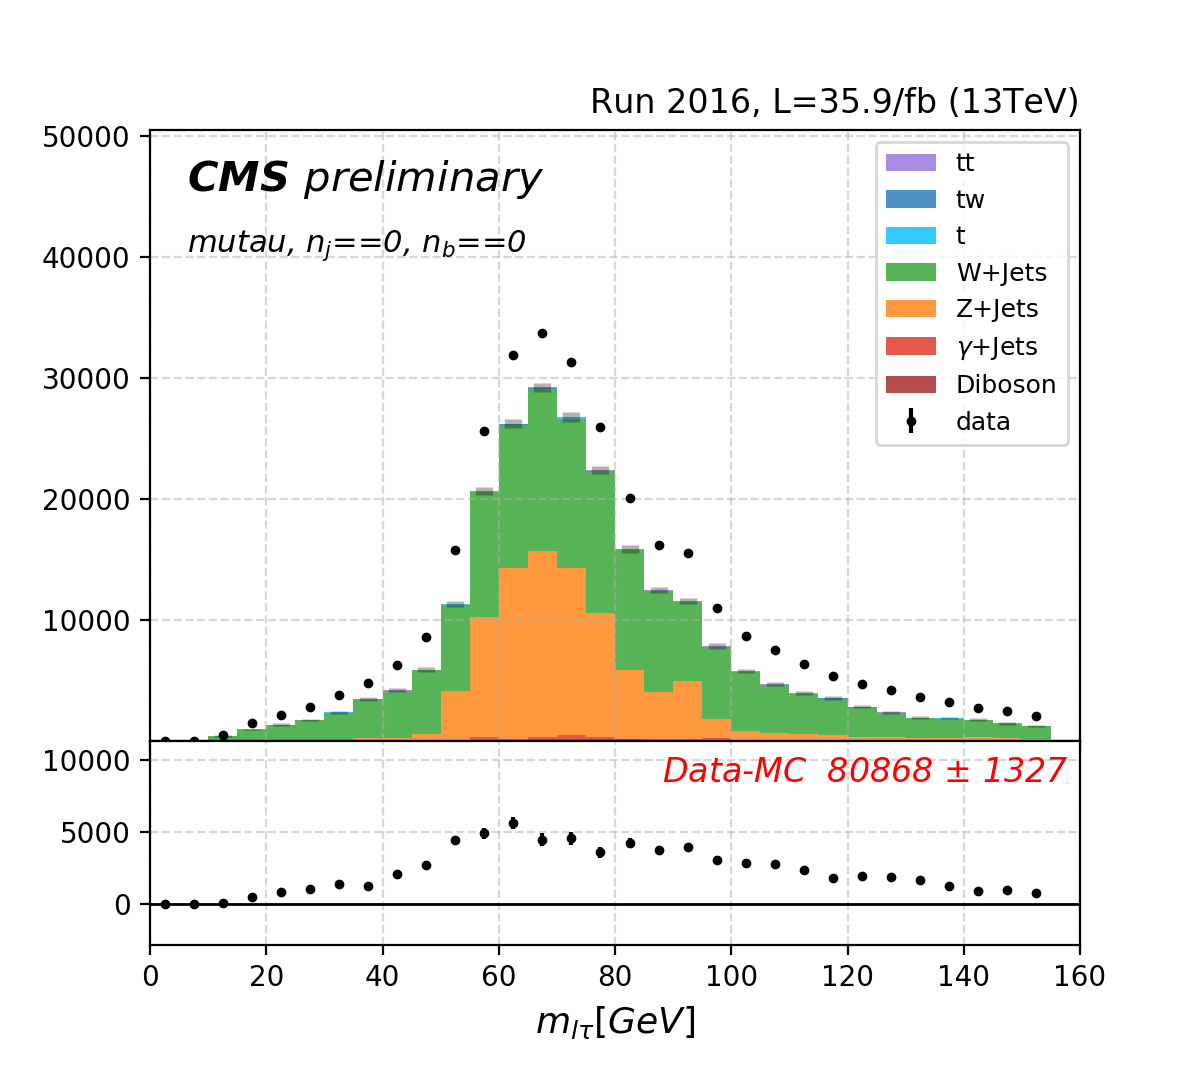
\includegraphics[width=0.24\textwidth]{appendices/qcdSF/figures/mutau_==0_==0_dilepton_mass.png}
    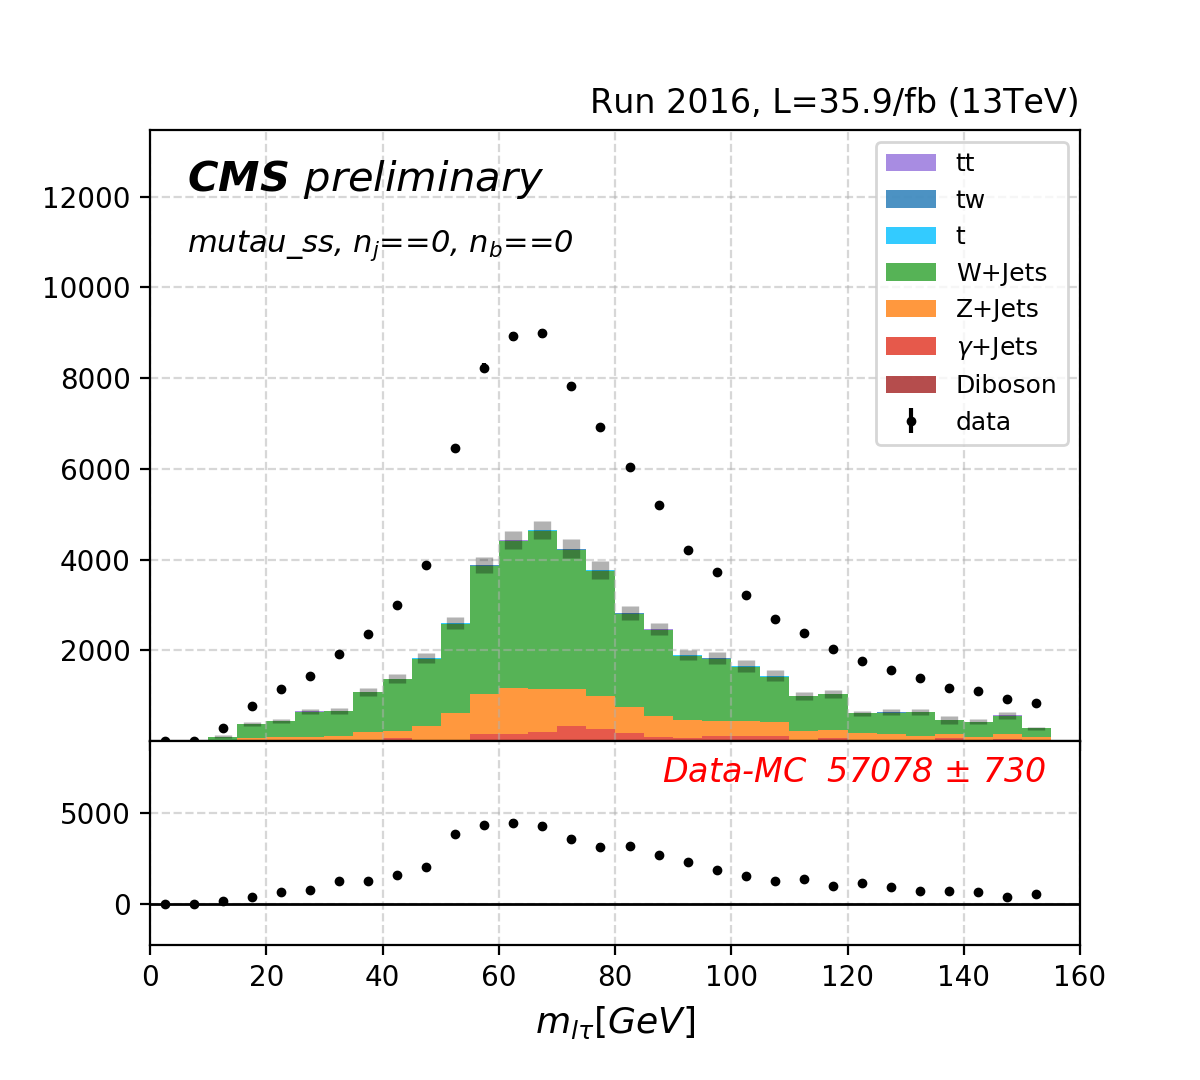
\includegraphics[width=0.24\textwidth]{appendices/qcdSF/figures/mutau_ss_==0_==0_dilepton_mass.png}
    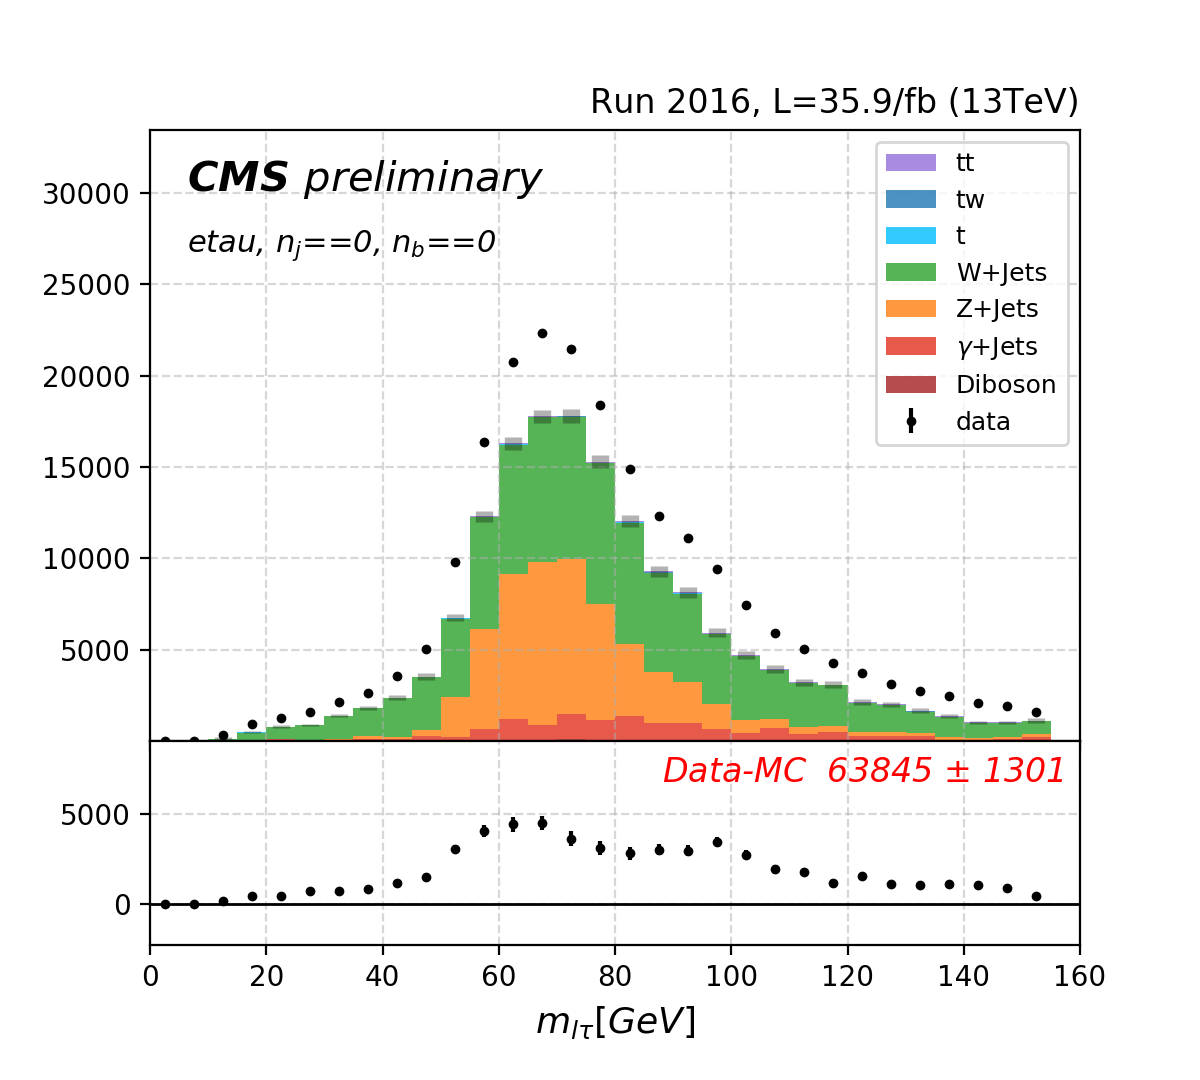
\includegraphics[width=0.24\textwidth]{appendices/qcdSF/figures/etau_==0_==0_dilepton_mass.png}
    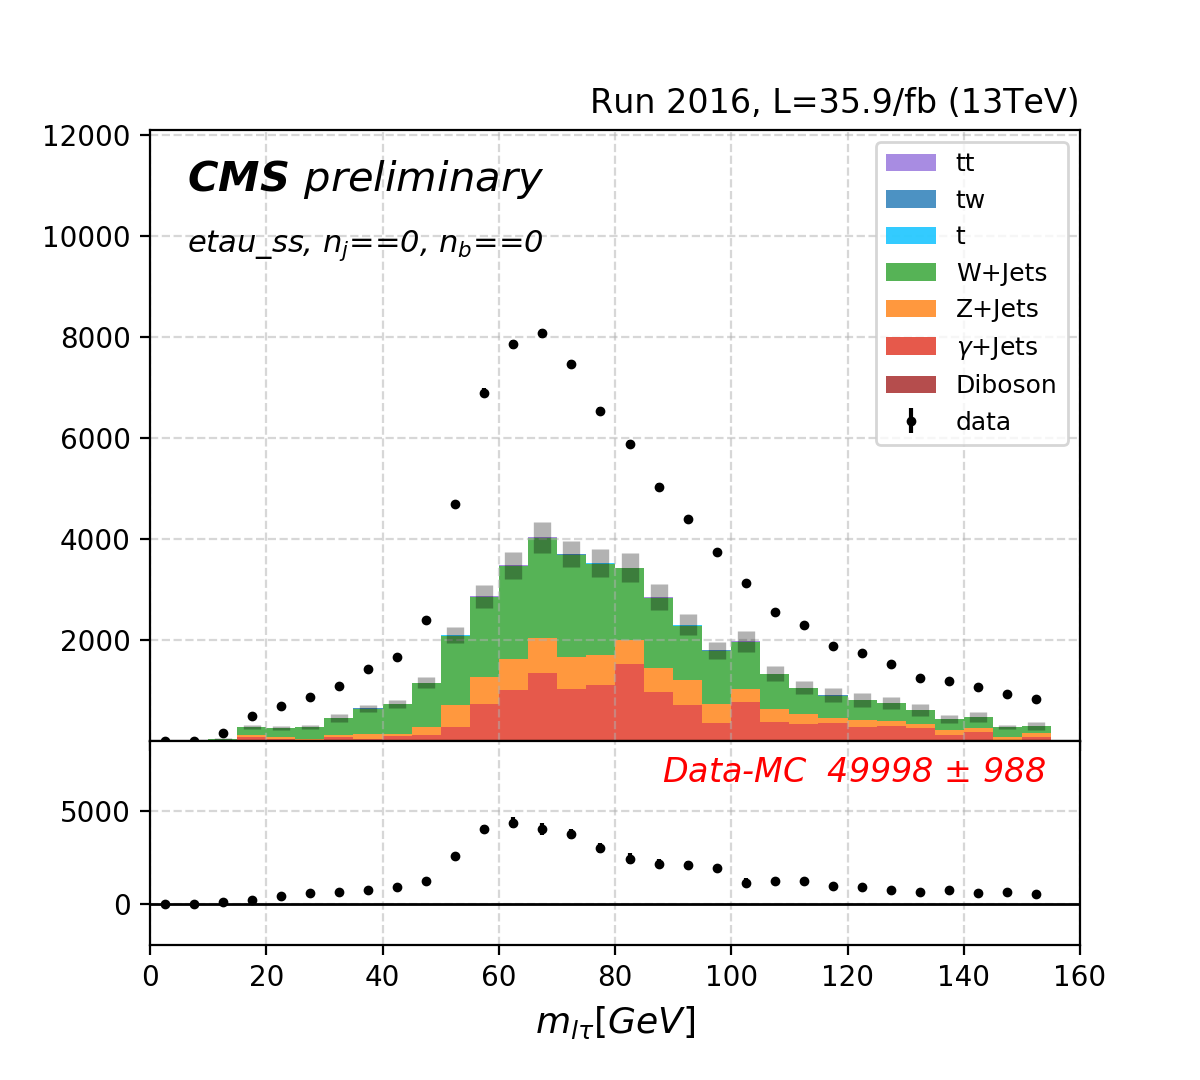
\includegraphics[width=0.24\textwidth]{appendices/qcdSF/figures/etau_ss_==0_==0_dilepton_mass.png}
    
    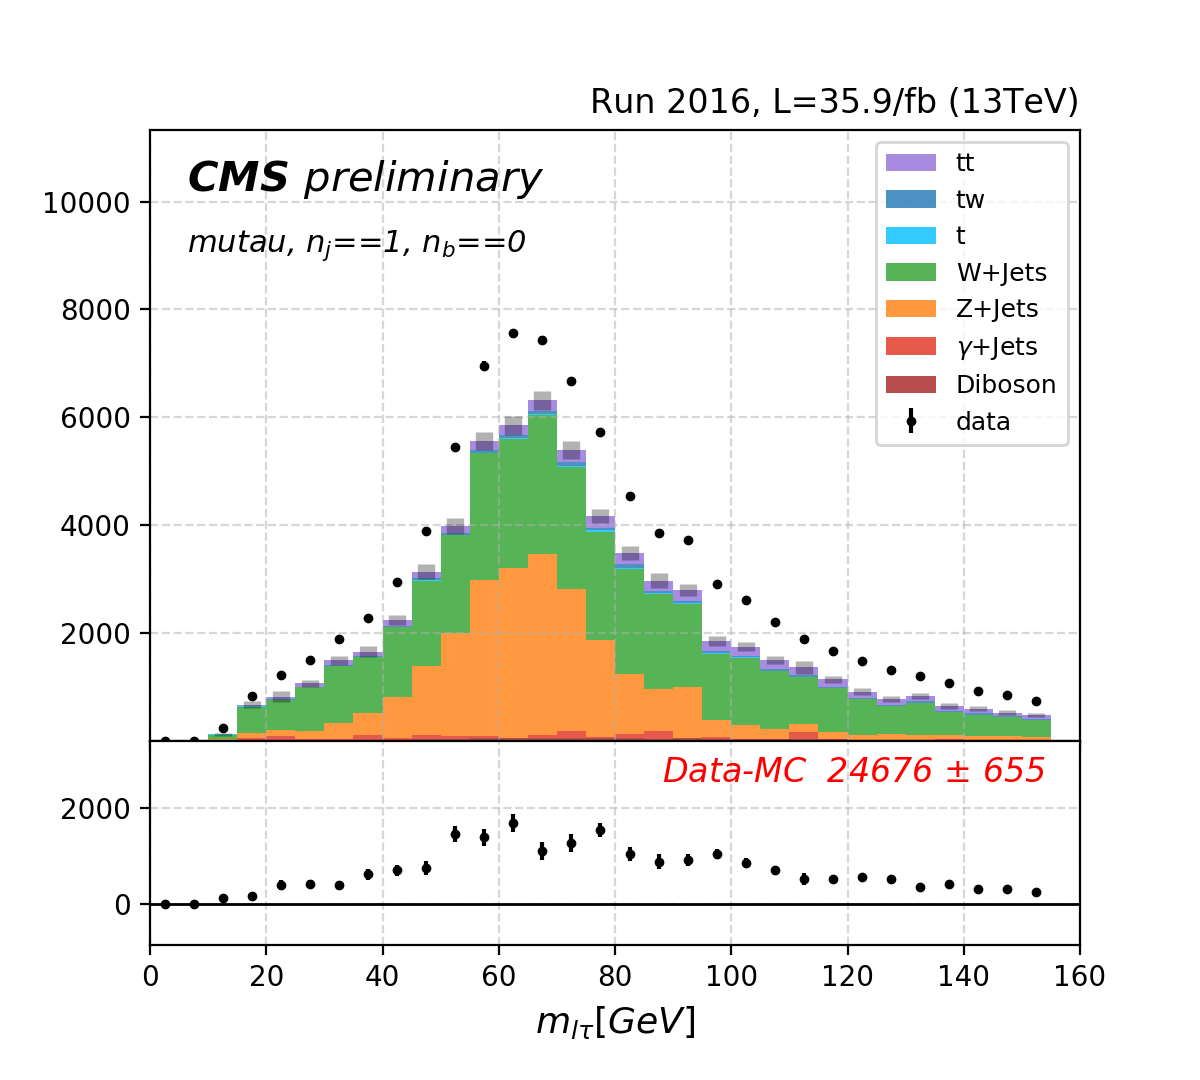
\includegraphics[width=0.24\textwidth]{appendices/qcdSF/figures/mutau_==1_==0_dilepton_mass.png}
    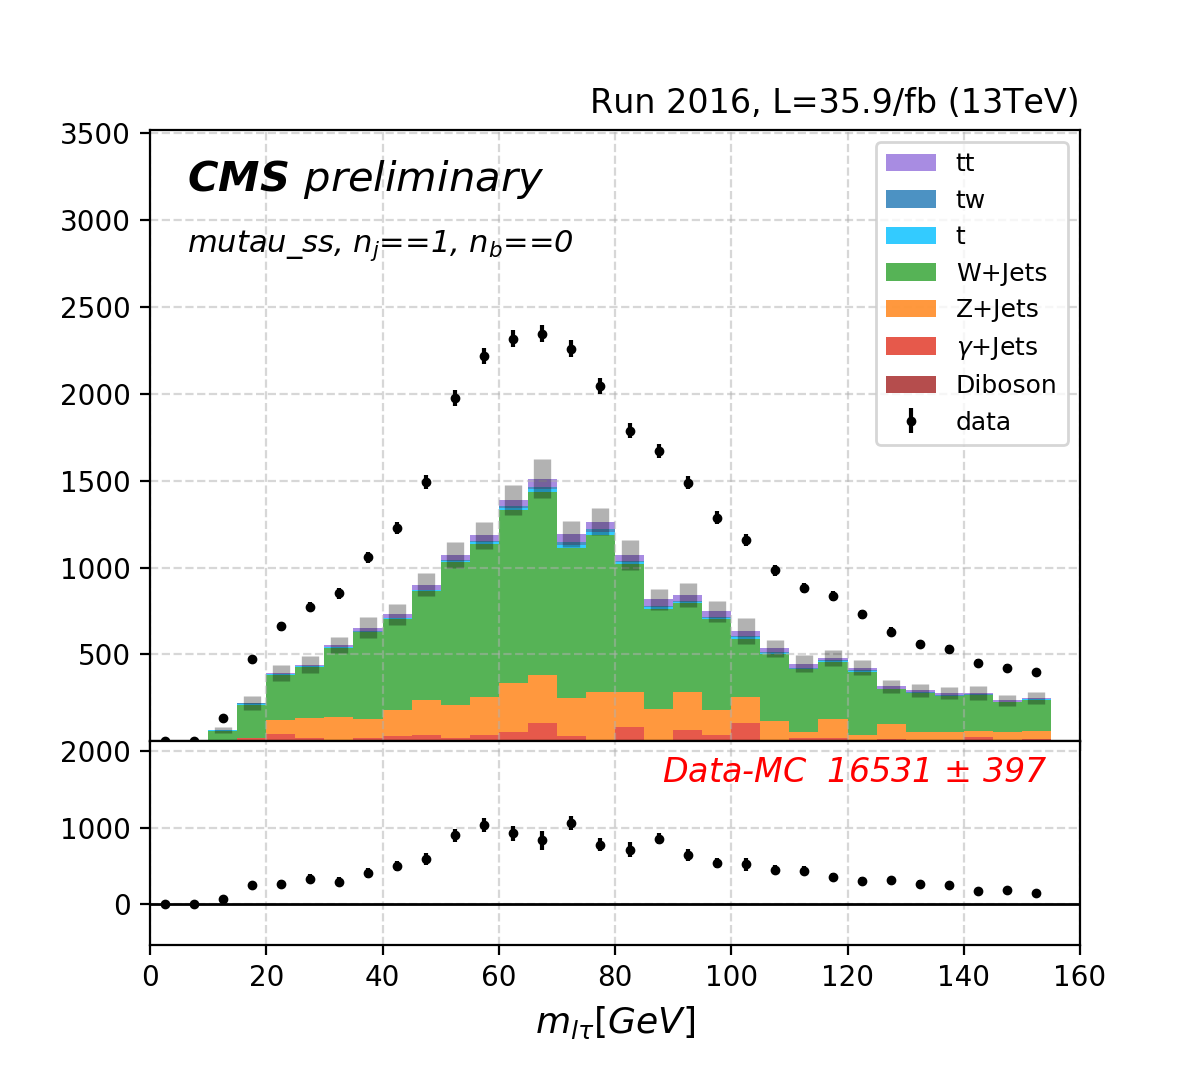
\includegraphics[width=0.24\textwidth]{appendices/qcdSF/figures/mutau_ss_==1_==0_dilepton_mass.png}
    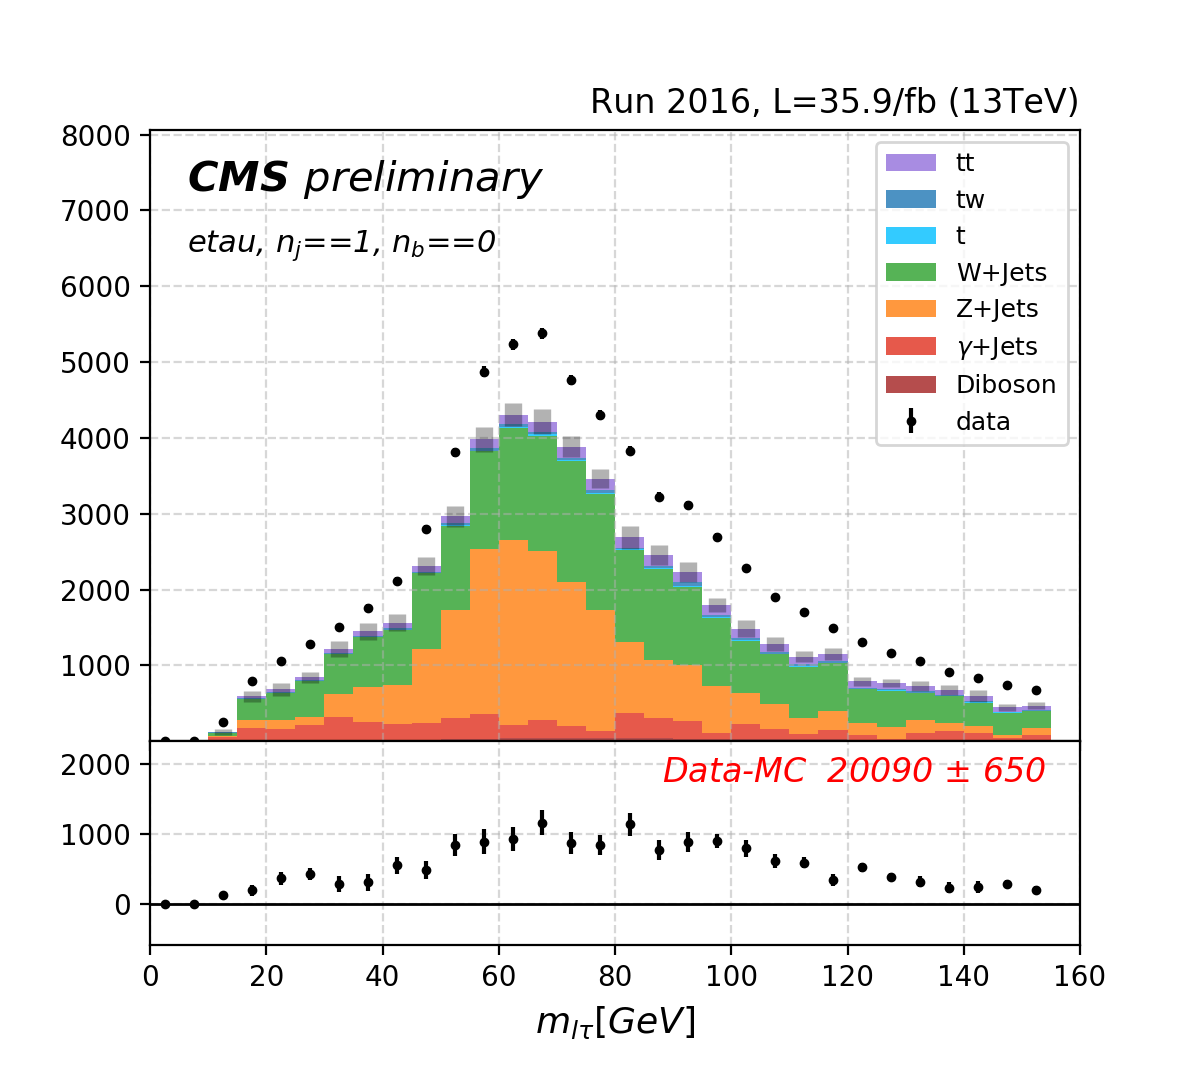
\includegraphics[width=0.24\textwidth]{appendices/qcdSF/figures/etau_==1_==0_dilepton_mass.png}
    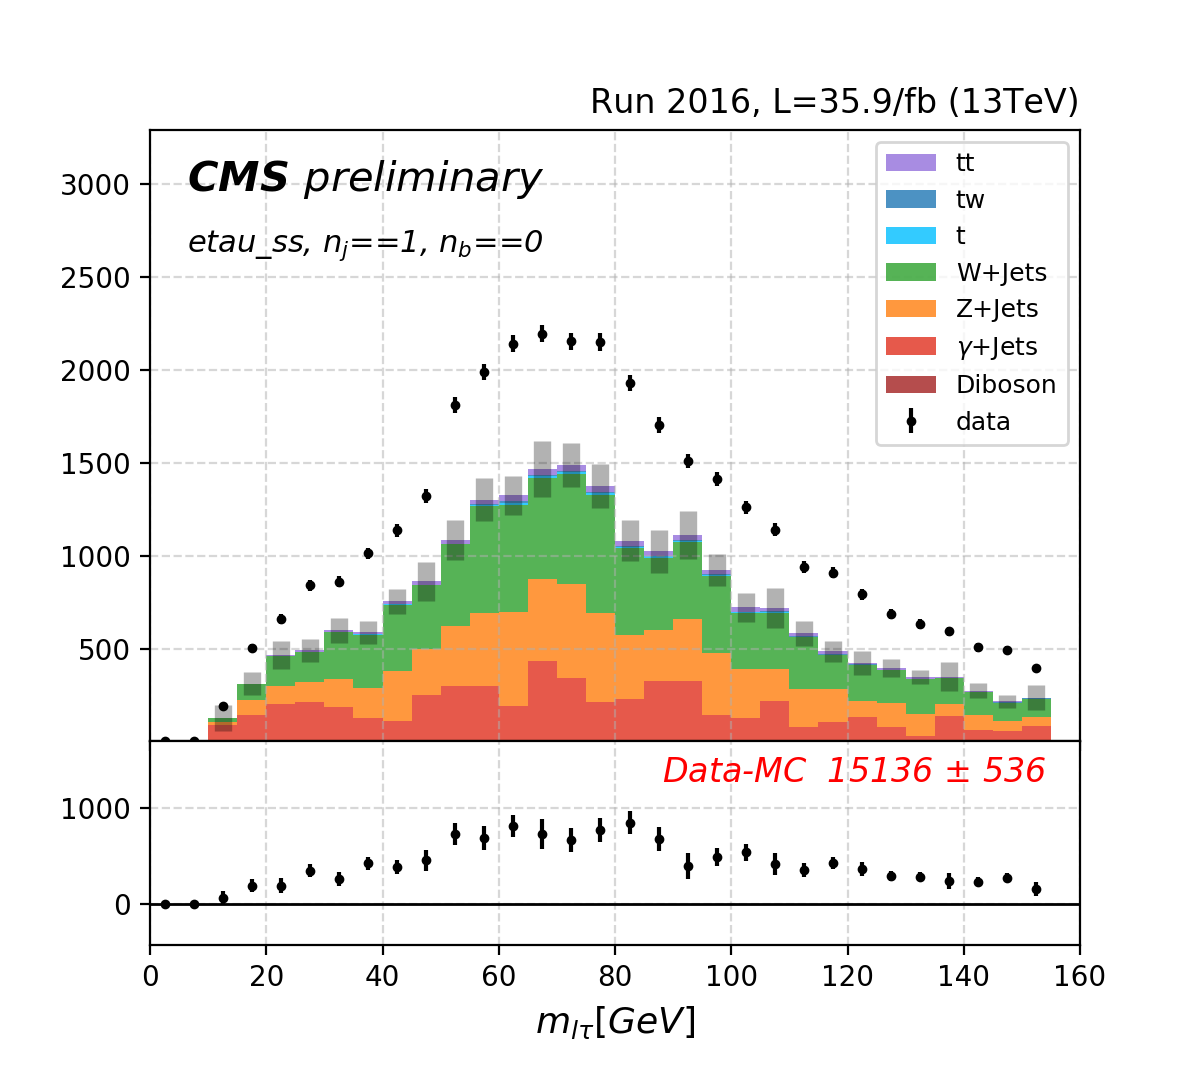
\includegraphics[width=0.24\textwidth]{appendices/qcdSF/figures/etau_ss_==1_==0_dilepton_mass.png}
    
    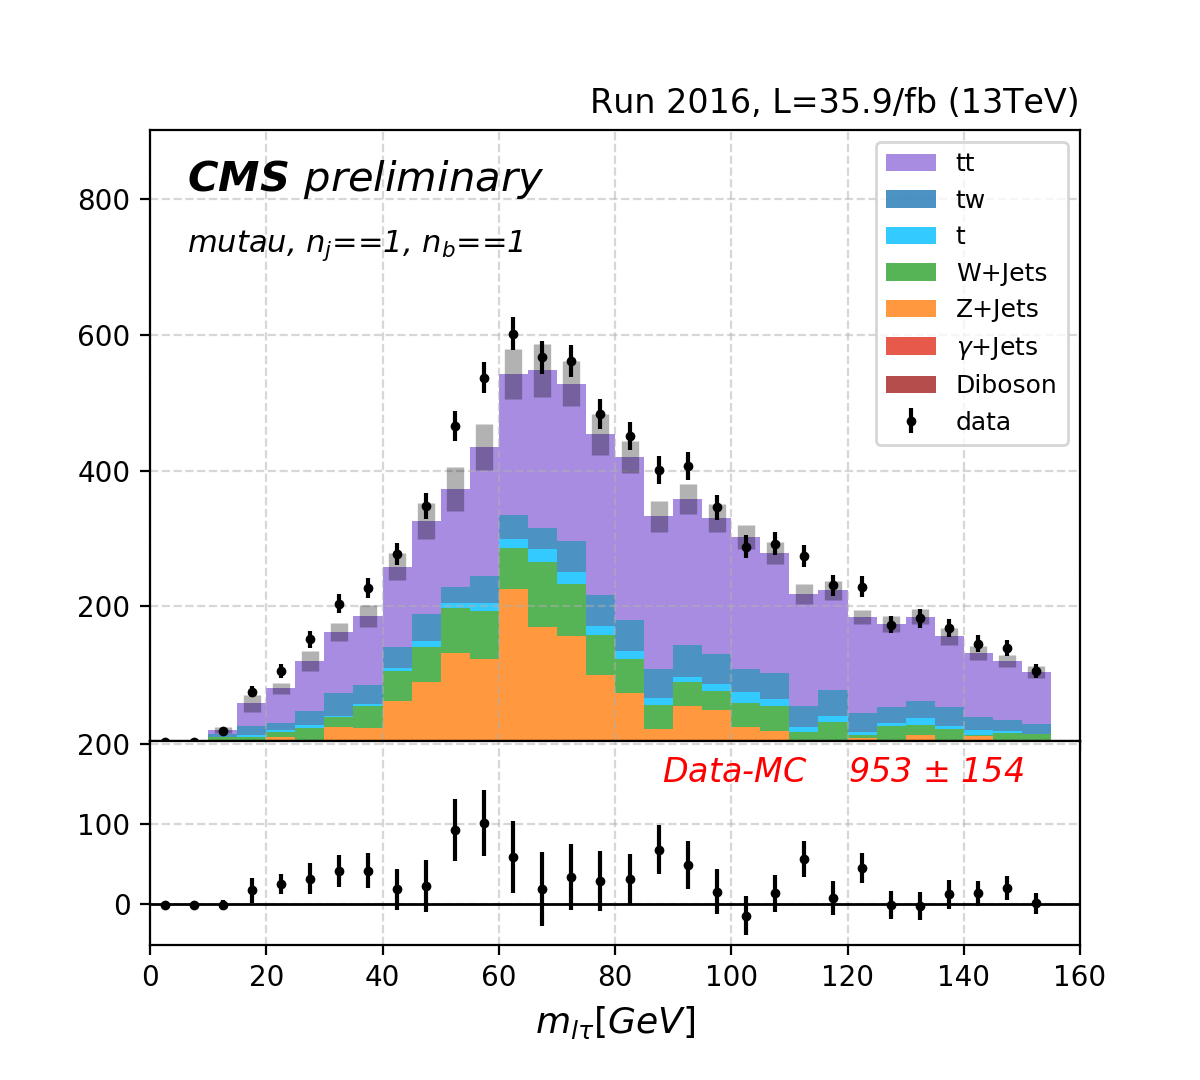
\includegraphics[width=0.24\textwidth]{appendices/qcdSF/figures/mutau_==1_==1_dilepton_mass.png}
    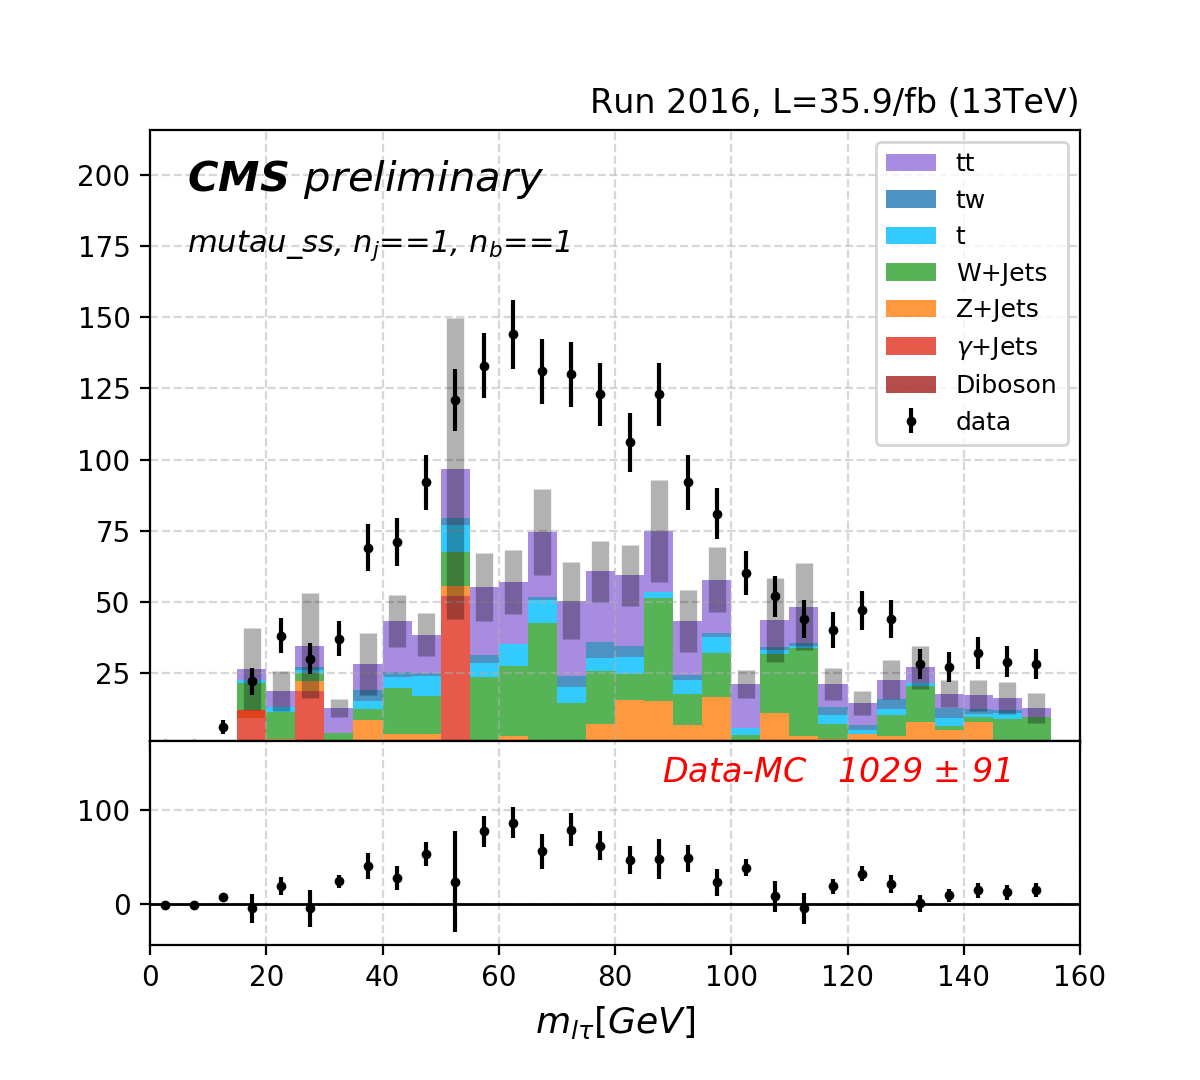
\includegraphics[width=0.24\textwidth]{appendices/qcdSF/figures/mutau_ss_==1_==1_dilepton_mass.png}
    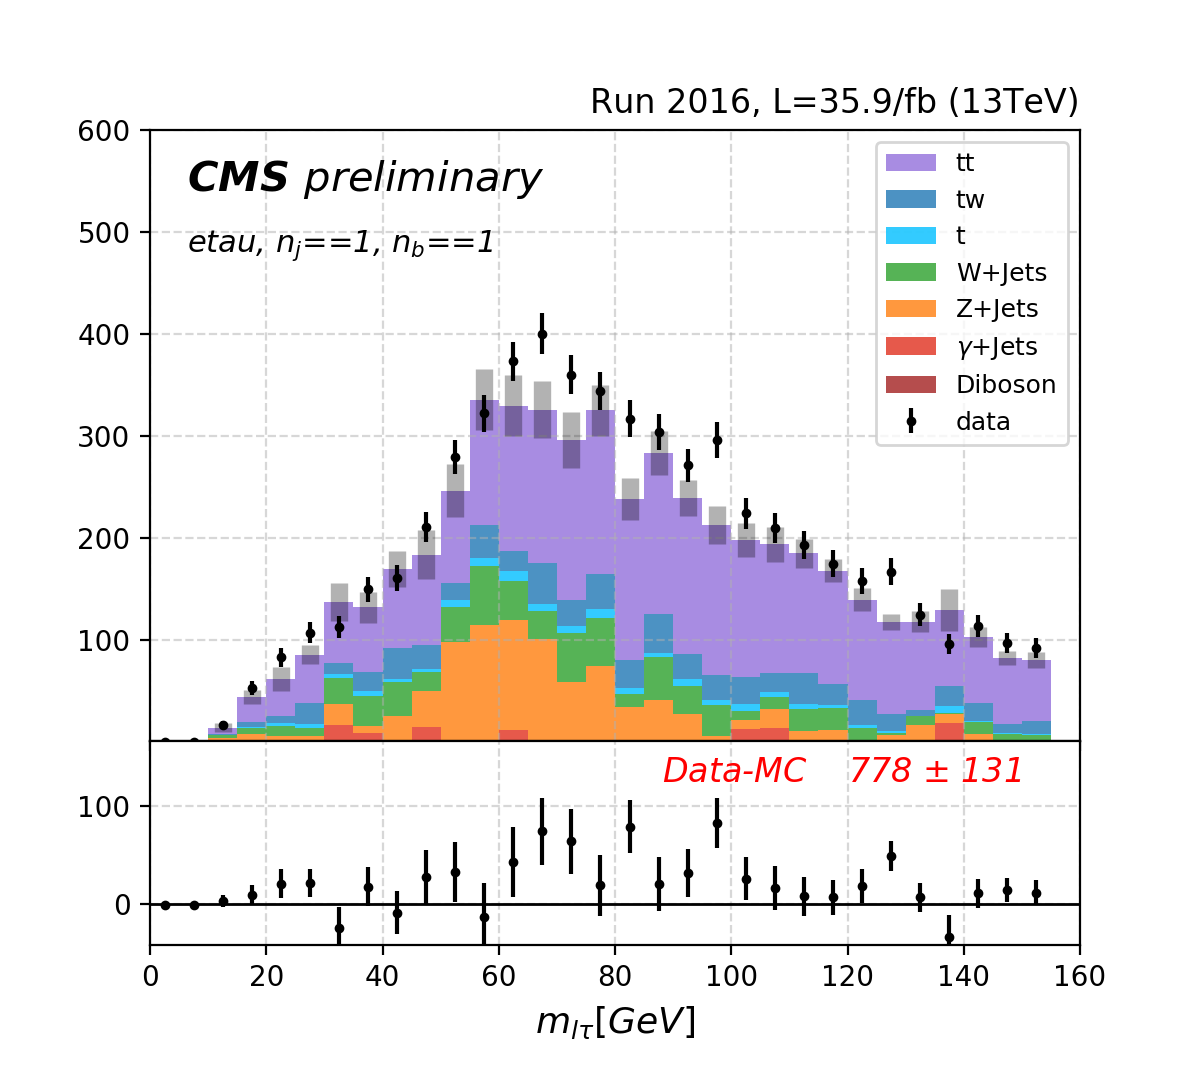
\includegraphics[width=0.24\textwidth]{appendices/qcdSF/figures/etau_==1_==1_dilepton_mass.png}
    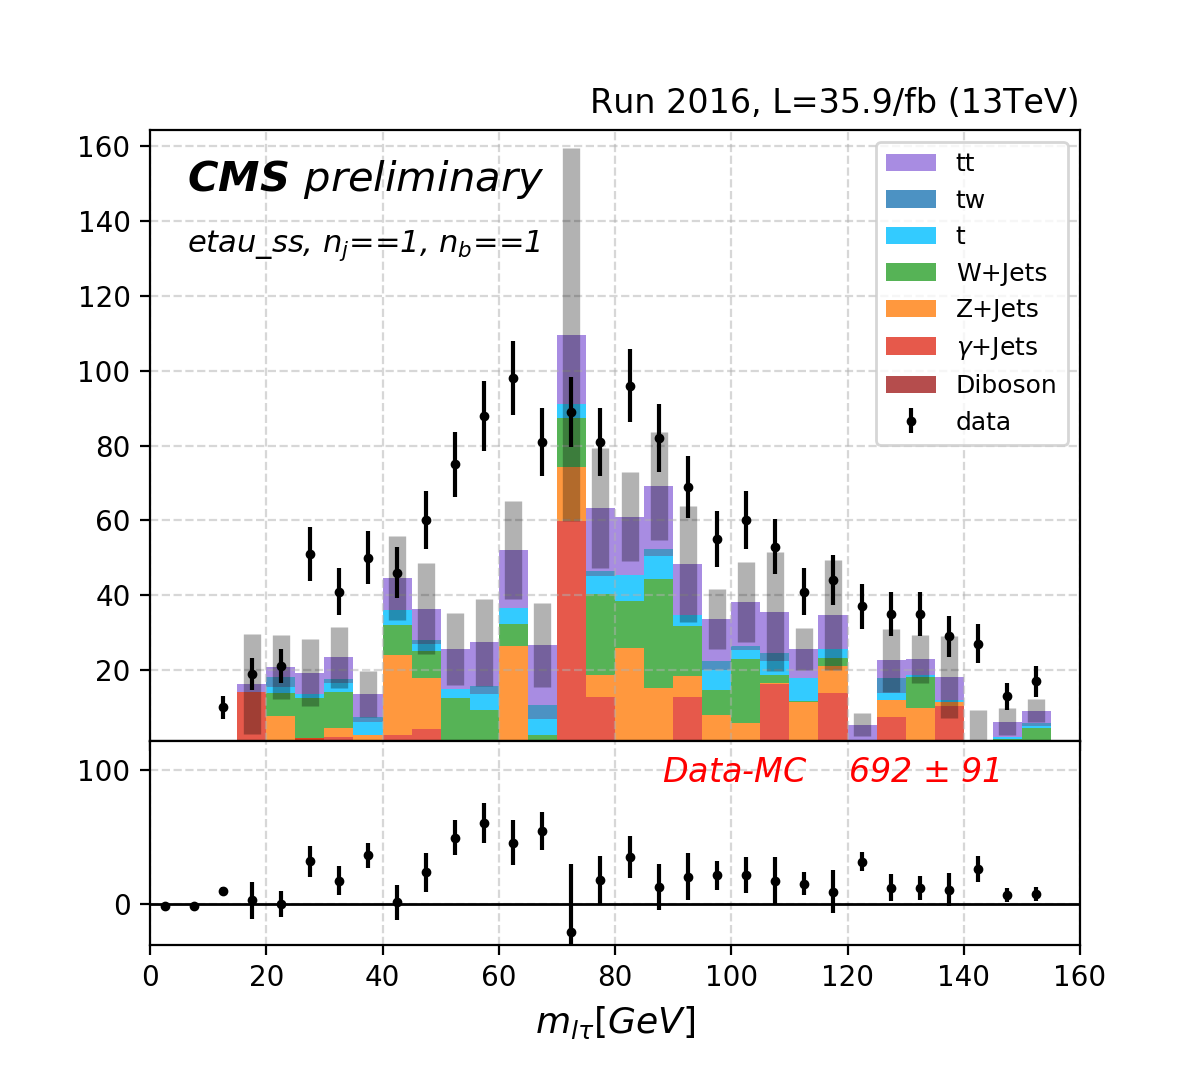
\includegraphics[width=0.24\textwidth]{appendices/qcdSF/figures/etau_ss_==1_==1_dilepton_mass.png}
    
    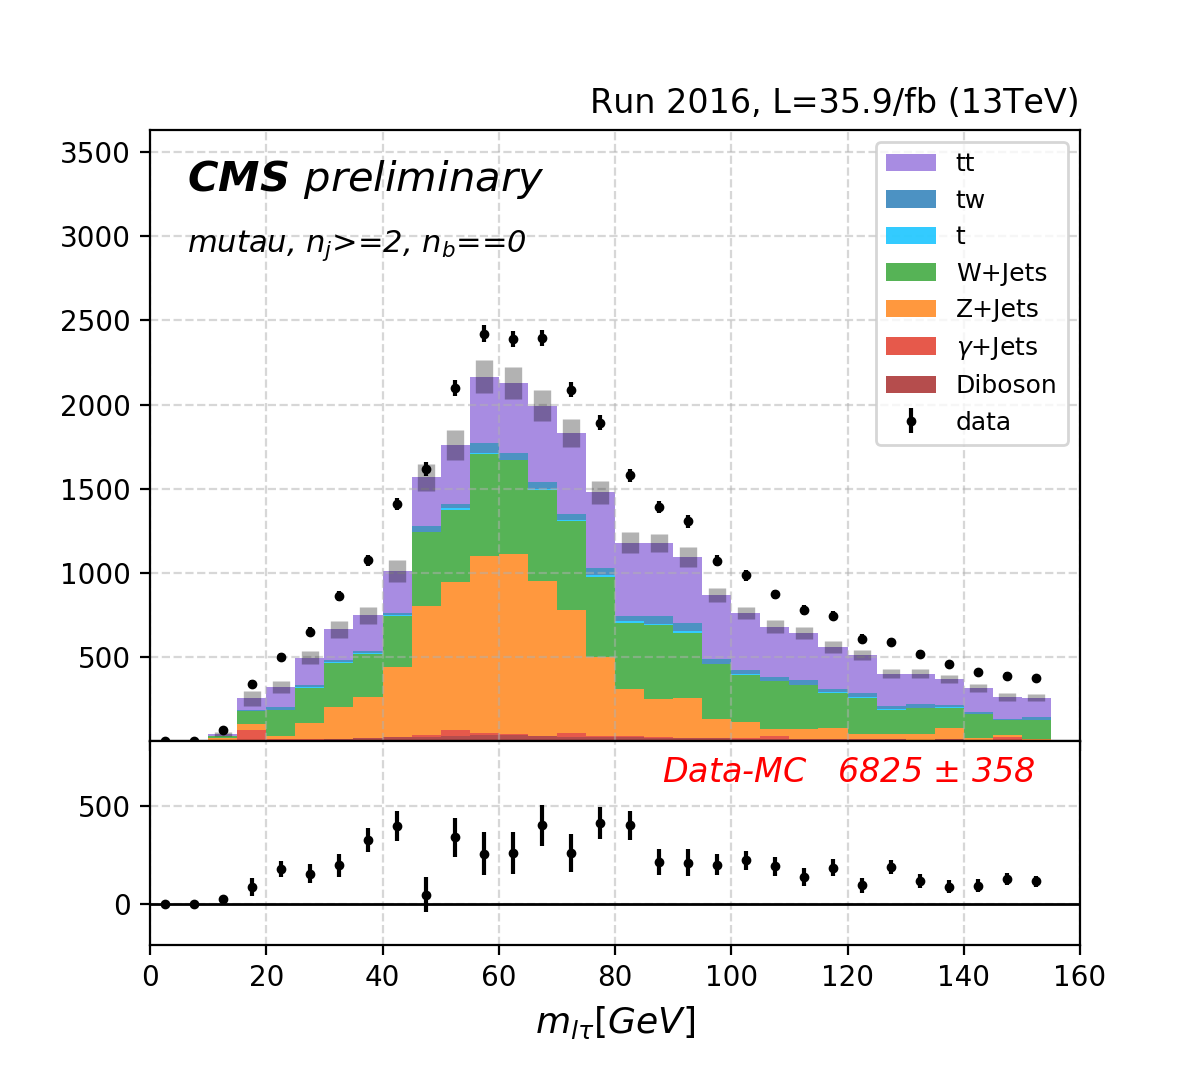
\includegraphics[width=0.24\textwidth]{appendices/qcdSF/figures/mutau_>=2_==0_dilepton_mass.png}
    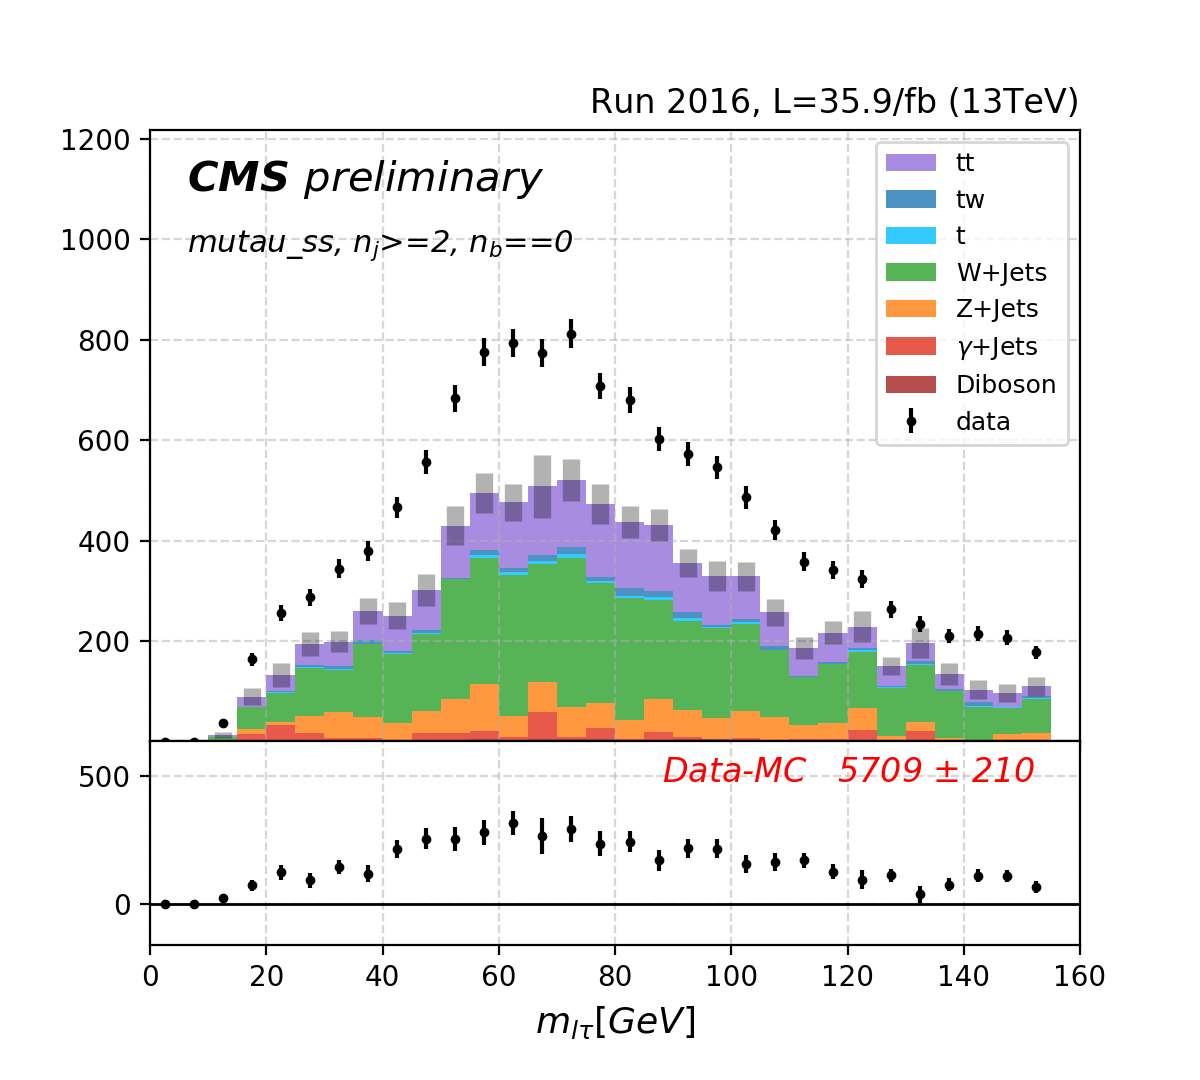
\includegraphics[width=0.24\textwidth]{appendices/qcdSF/figures/mutau_ss_>=2_==0_dilepton_mass.png}
    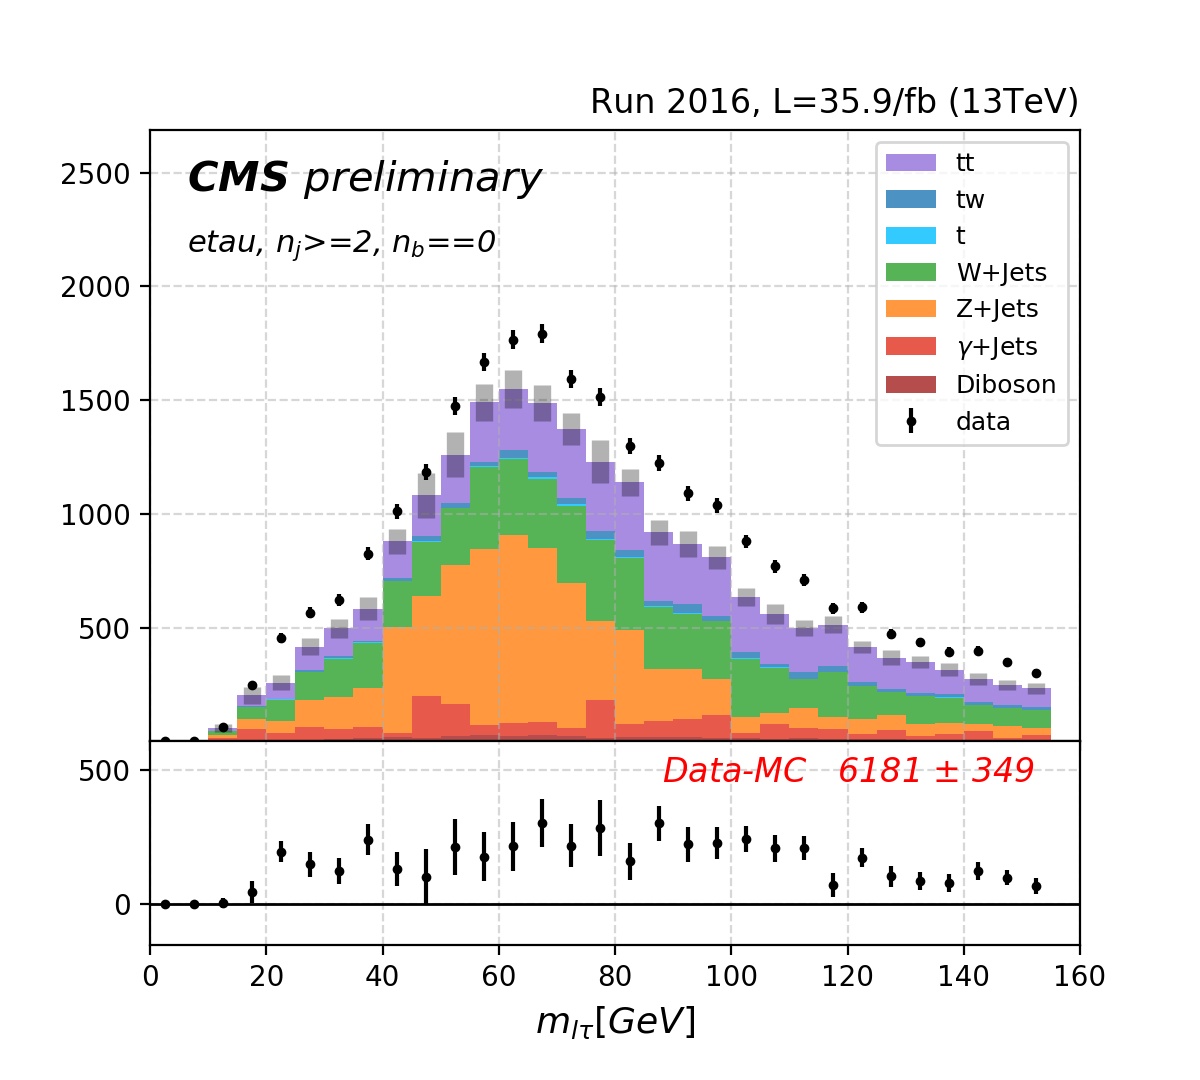
\includegraphics[width=0.24\textwidth]{appendices/qcdSF/figures/etau_>=2_==0_dilepton_mass.png}
    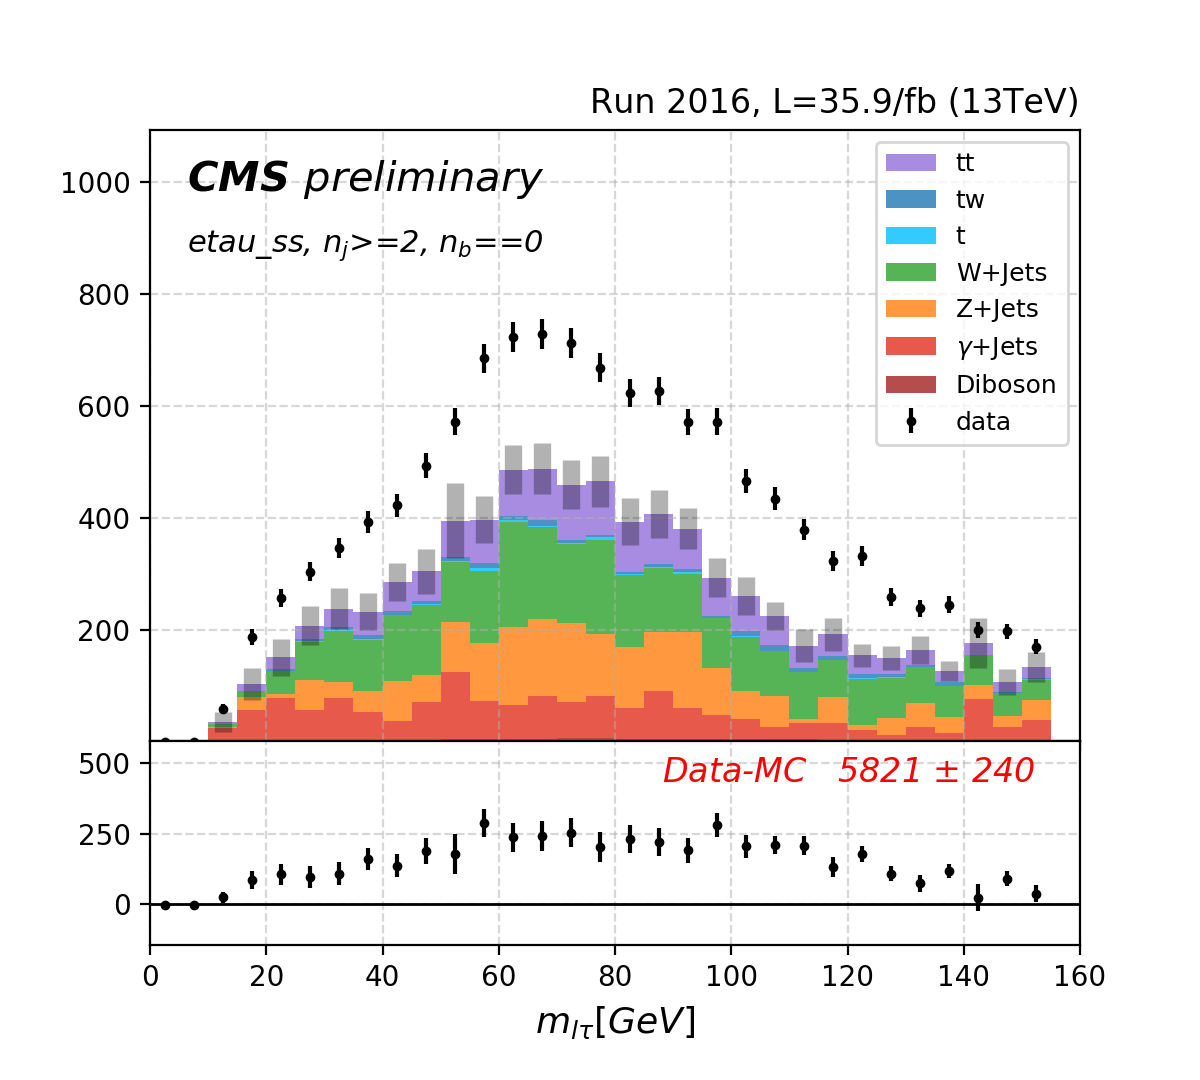
\includegraphics[width=0.24\textwidth]{appendices/qcdSF/figures/etau_ss_>=2_==0_dilepton_mass.png}
    
    
    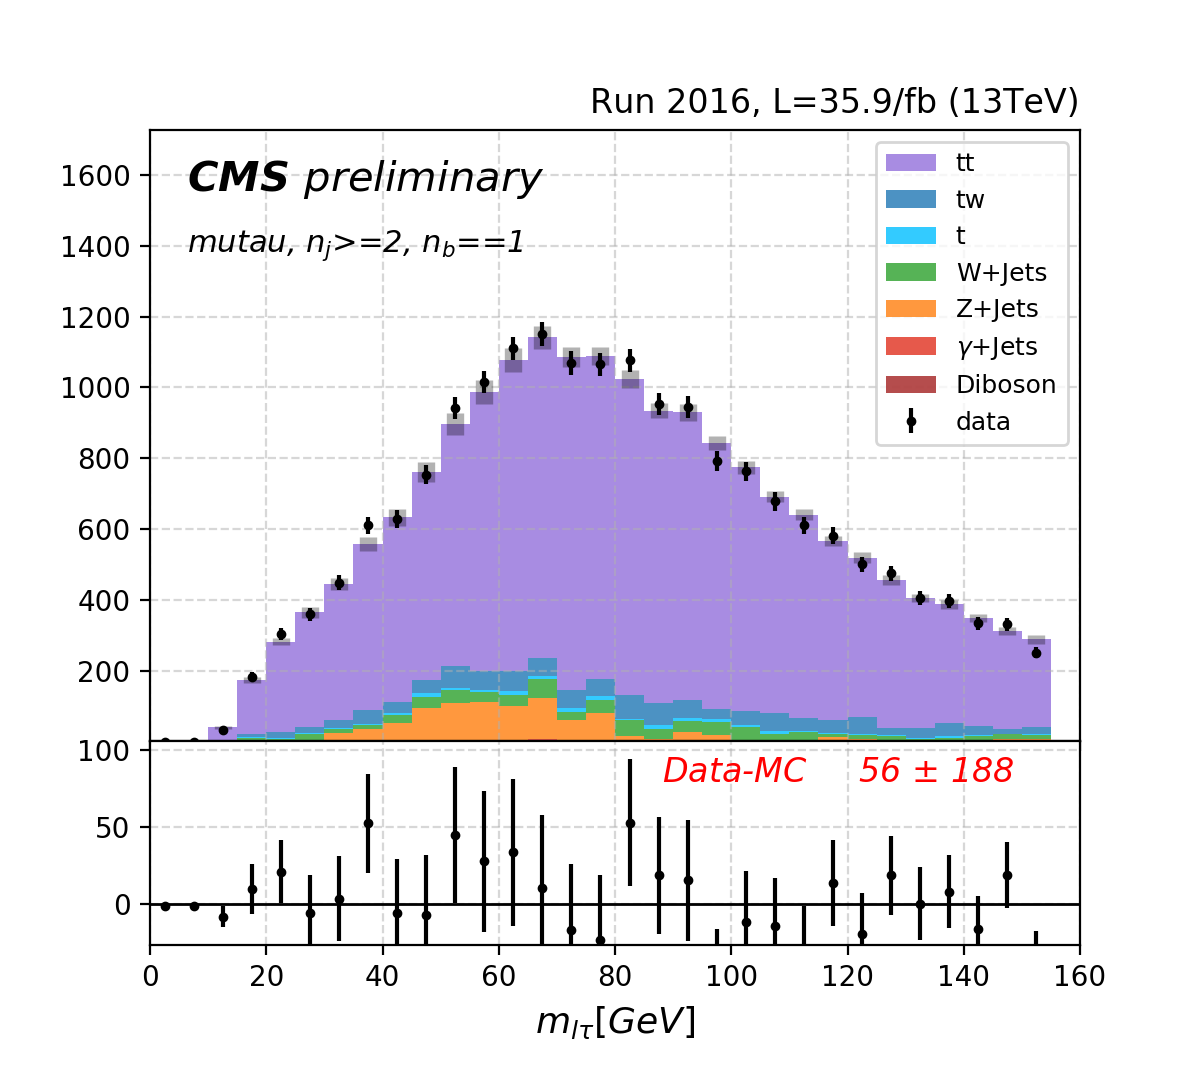
\includegraphics[width=0.24\textwidth]{appendices/qcdSF/figures/mutau_>=2_==1_dilepton_mass.png}
    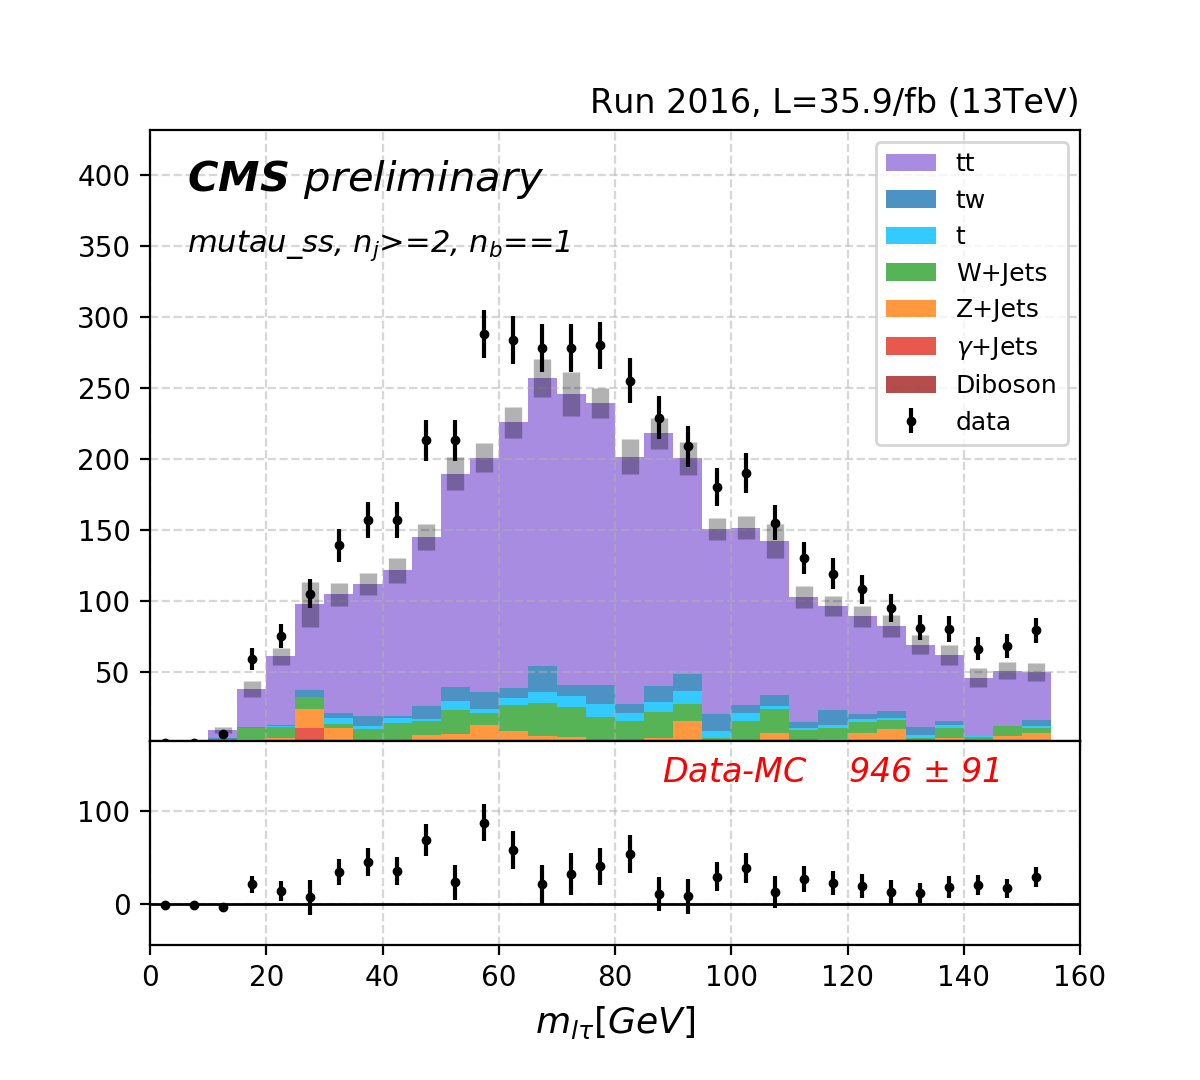
\includegraphics[width=0.24\textwidth]{appendices/qcdSF/figures/mutau_ss_>=2_==1_dilepton_mass.png}
    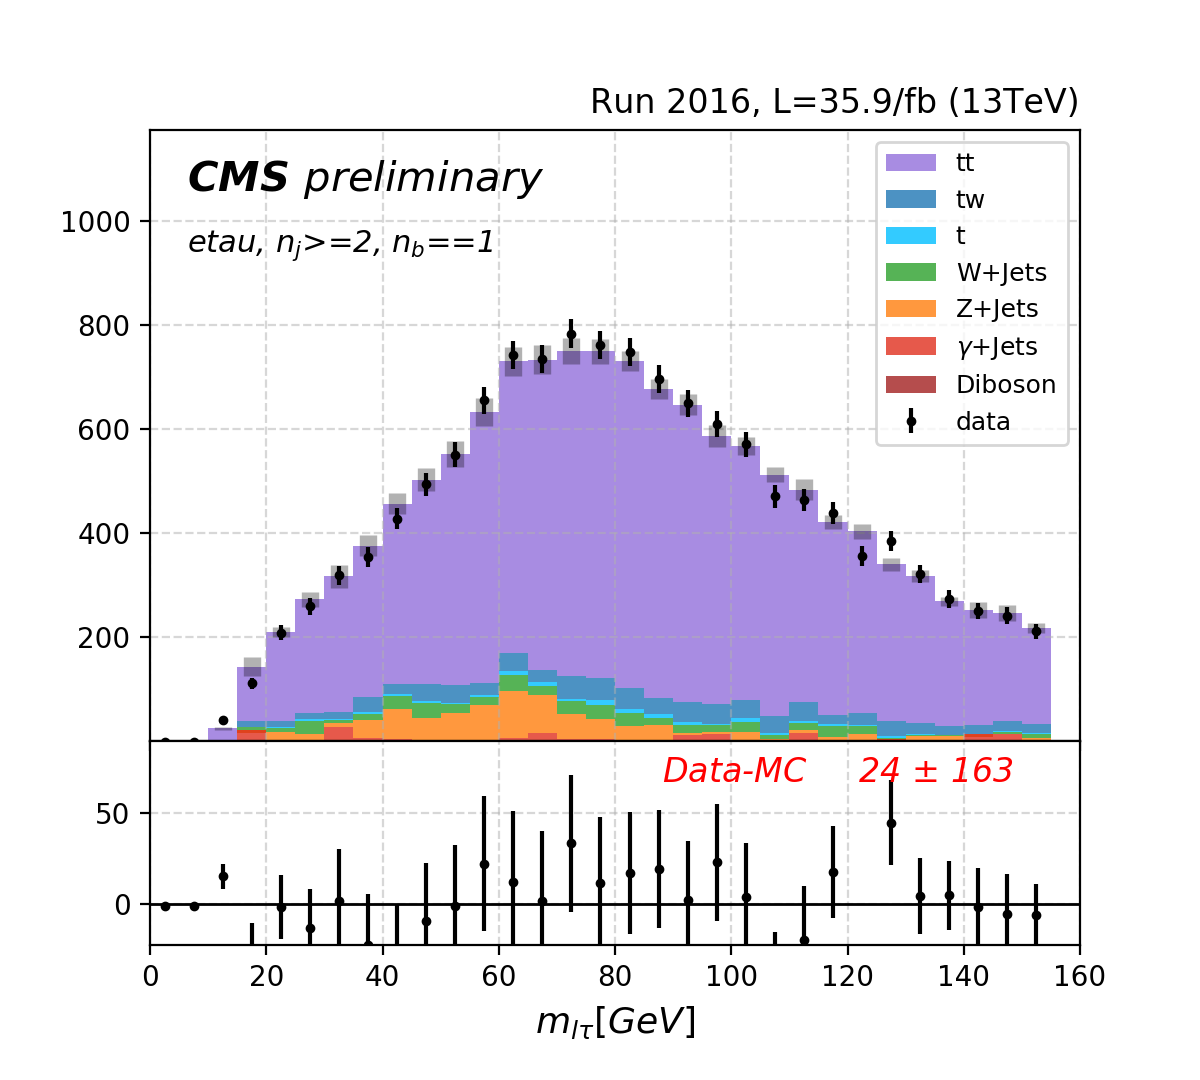
\includegraphics[width=0.24\textwidth]{appendices/qcdSF/figures/etau_>=2_==1_dilepton_mass.png}
    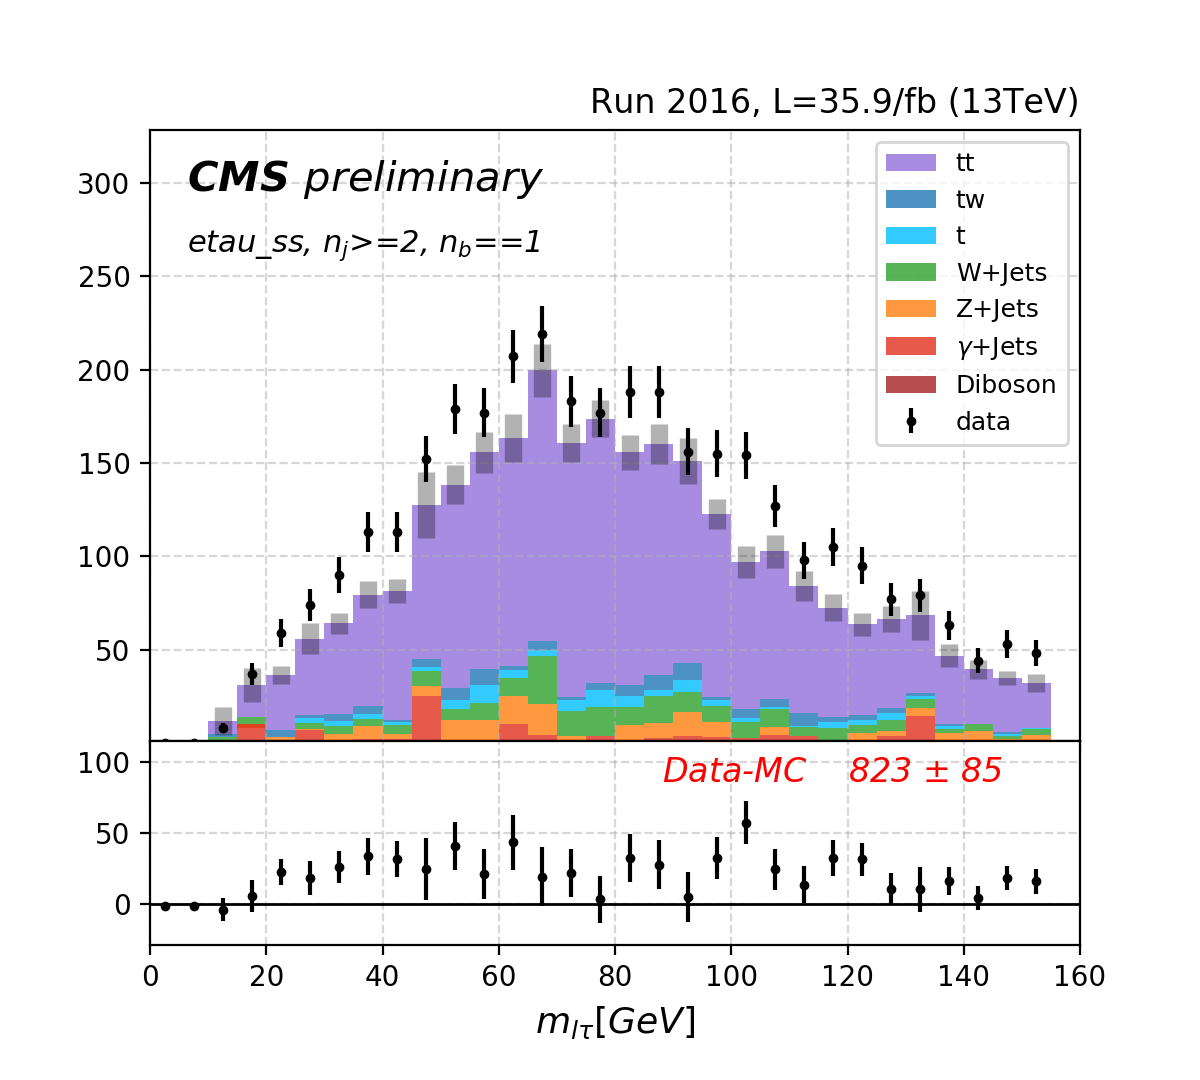
\includegraphics[width=0.24\textwidth]{appendices/qcdSF/figures/etau_ss_>=2_==1_dilepton_mass.png}
    
    
    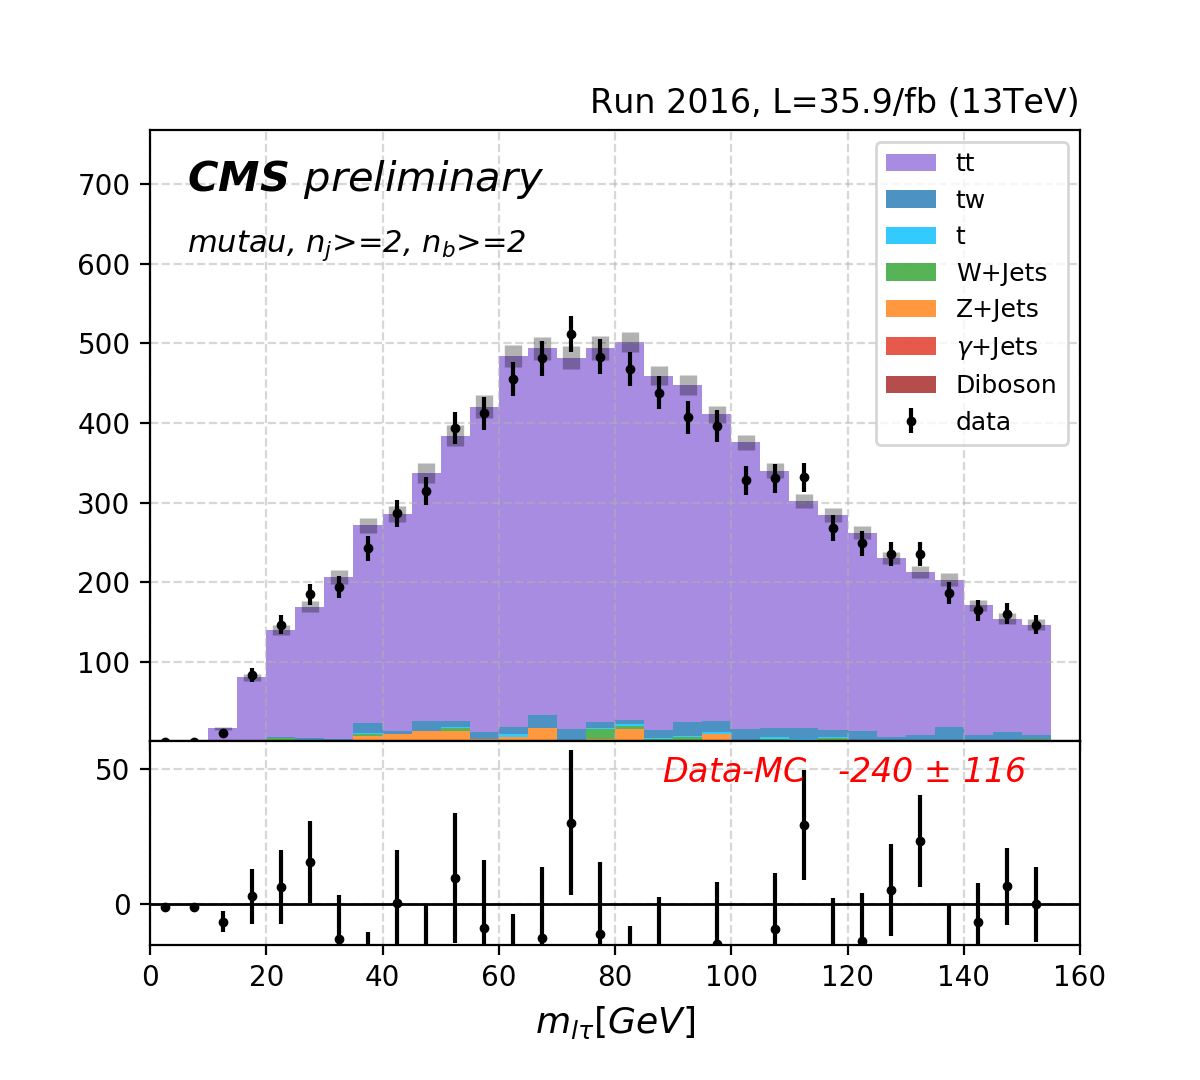
\includegraphics[width=0.24\textwidth]{appendices/qcdSF/figures/mutau_>=2_>=2_dilepton_mass.png}
    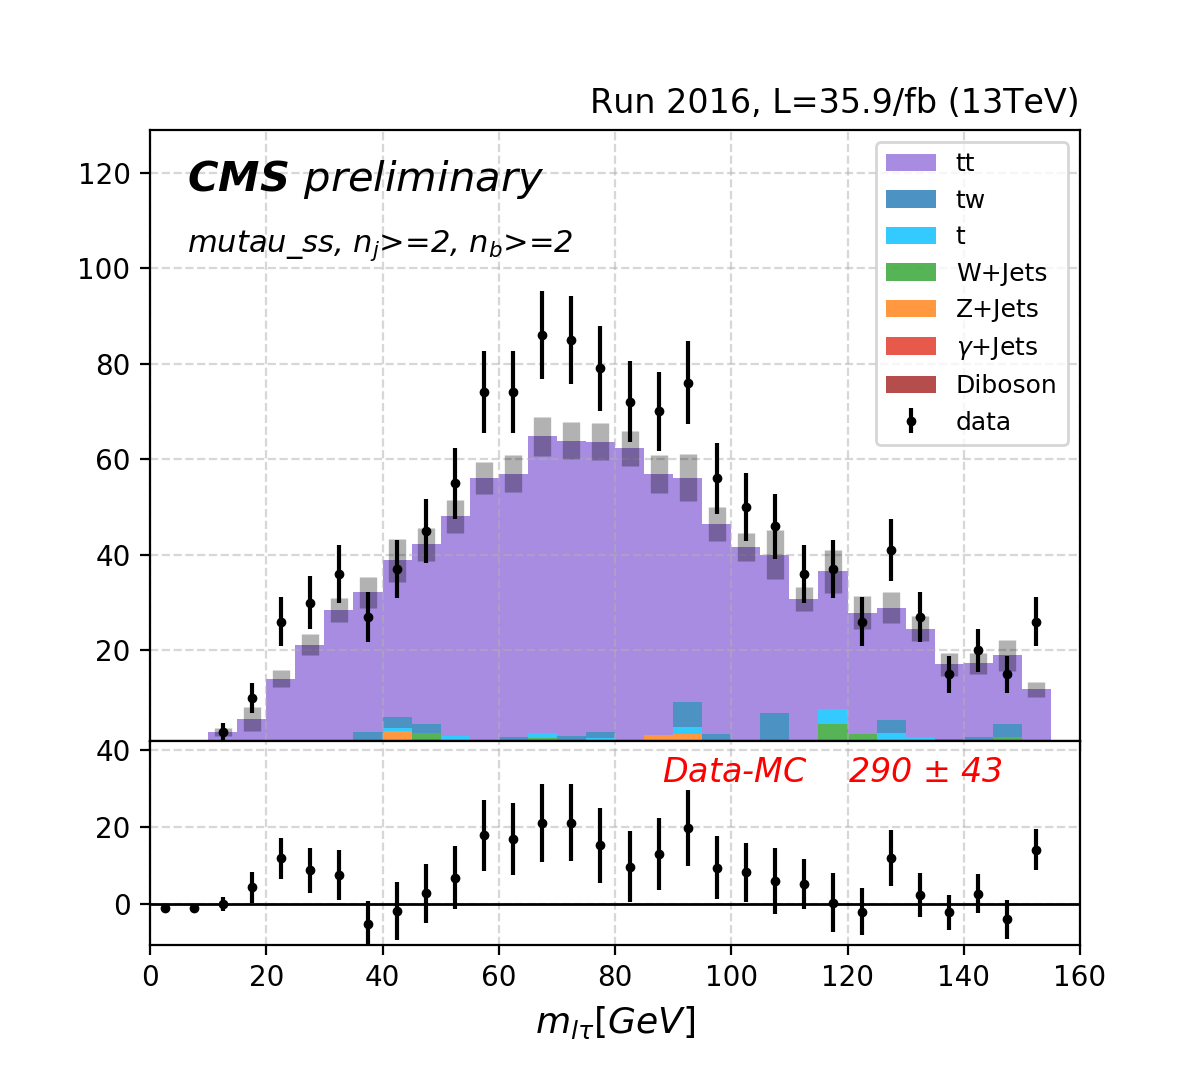
\includegraphics[width=0.24\textwidth]{appendices/qcdSF/figures/mutau_ss_>=2_>=2_dilepton_mass.png}
    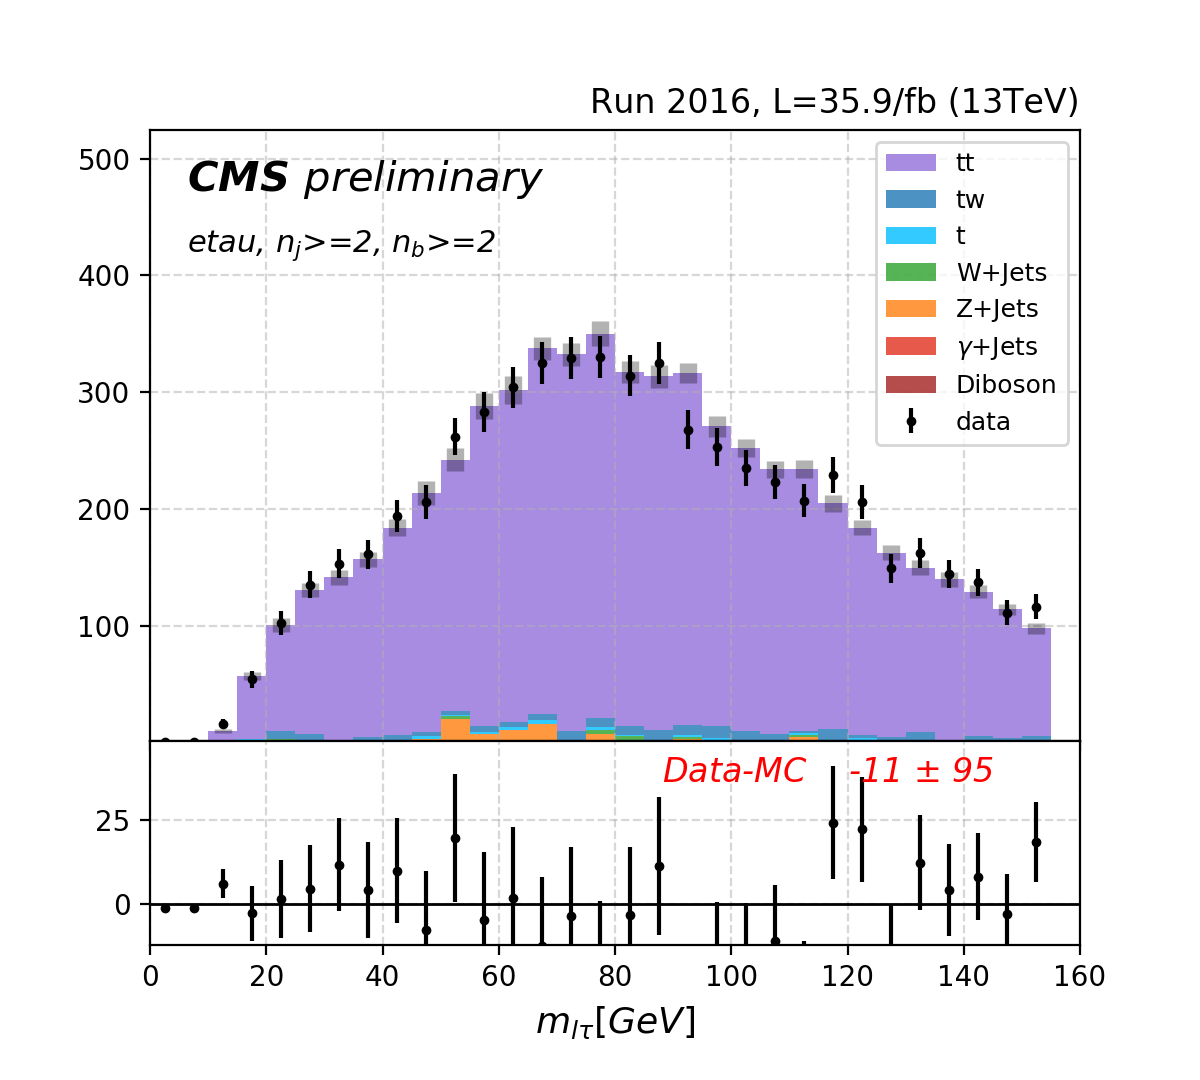
\includegraphics[width=0.24\textwidth]{appendices/qcdSF/figures/etau_>=2_>=2_dilepton_mass.png}
    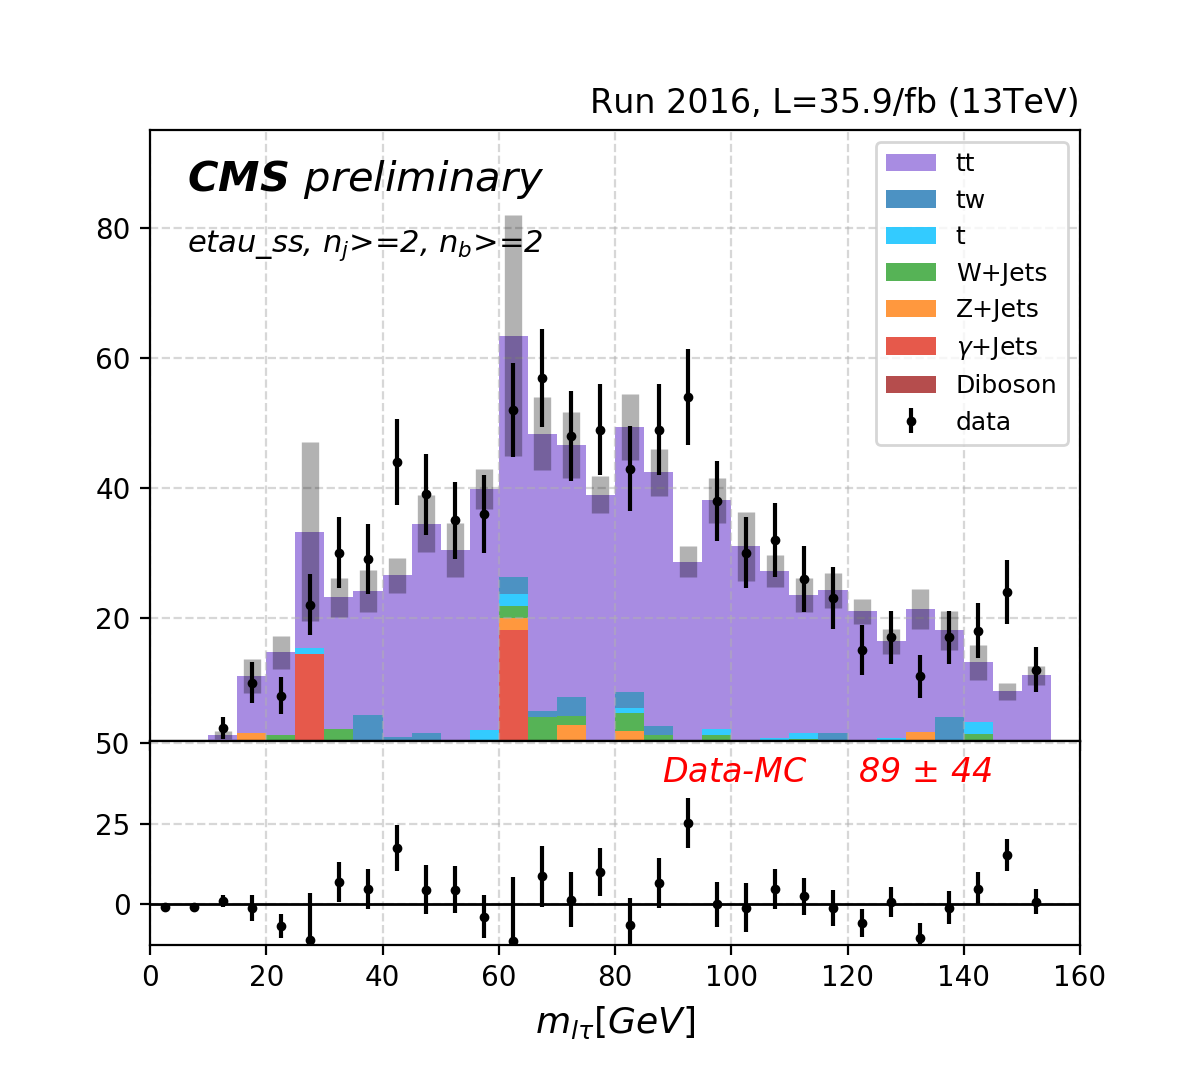
\includegraphics[width=0.24\textwidth]{appendices/qcdSF/figures/etau_ss_>=2_>=2_dilepton_mass.png}
    
    

    \caption{Reweight $\tau_h$ and $j \to \tau_h$ efficiencies in the dedicated FSR, ISF, MEPS, UE ttbar samples}
    \label{fig:appendix:qcdsf:ltau}
\end{figure}



\begin{figure}
    \centering
    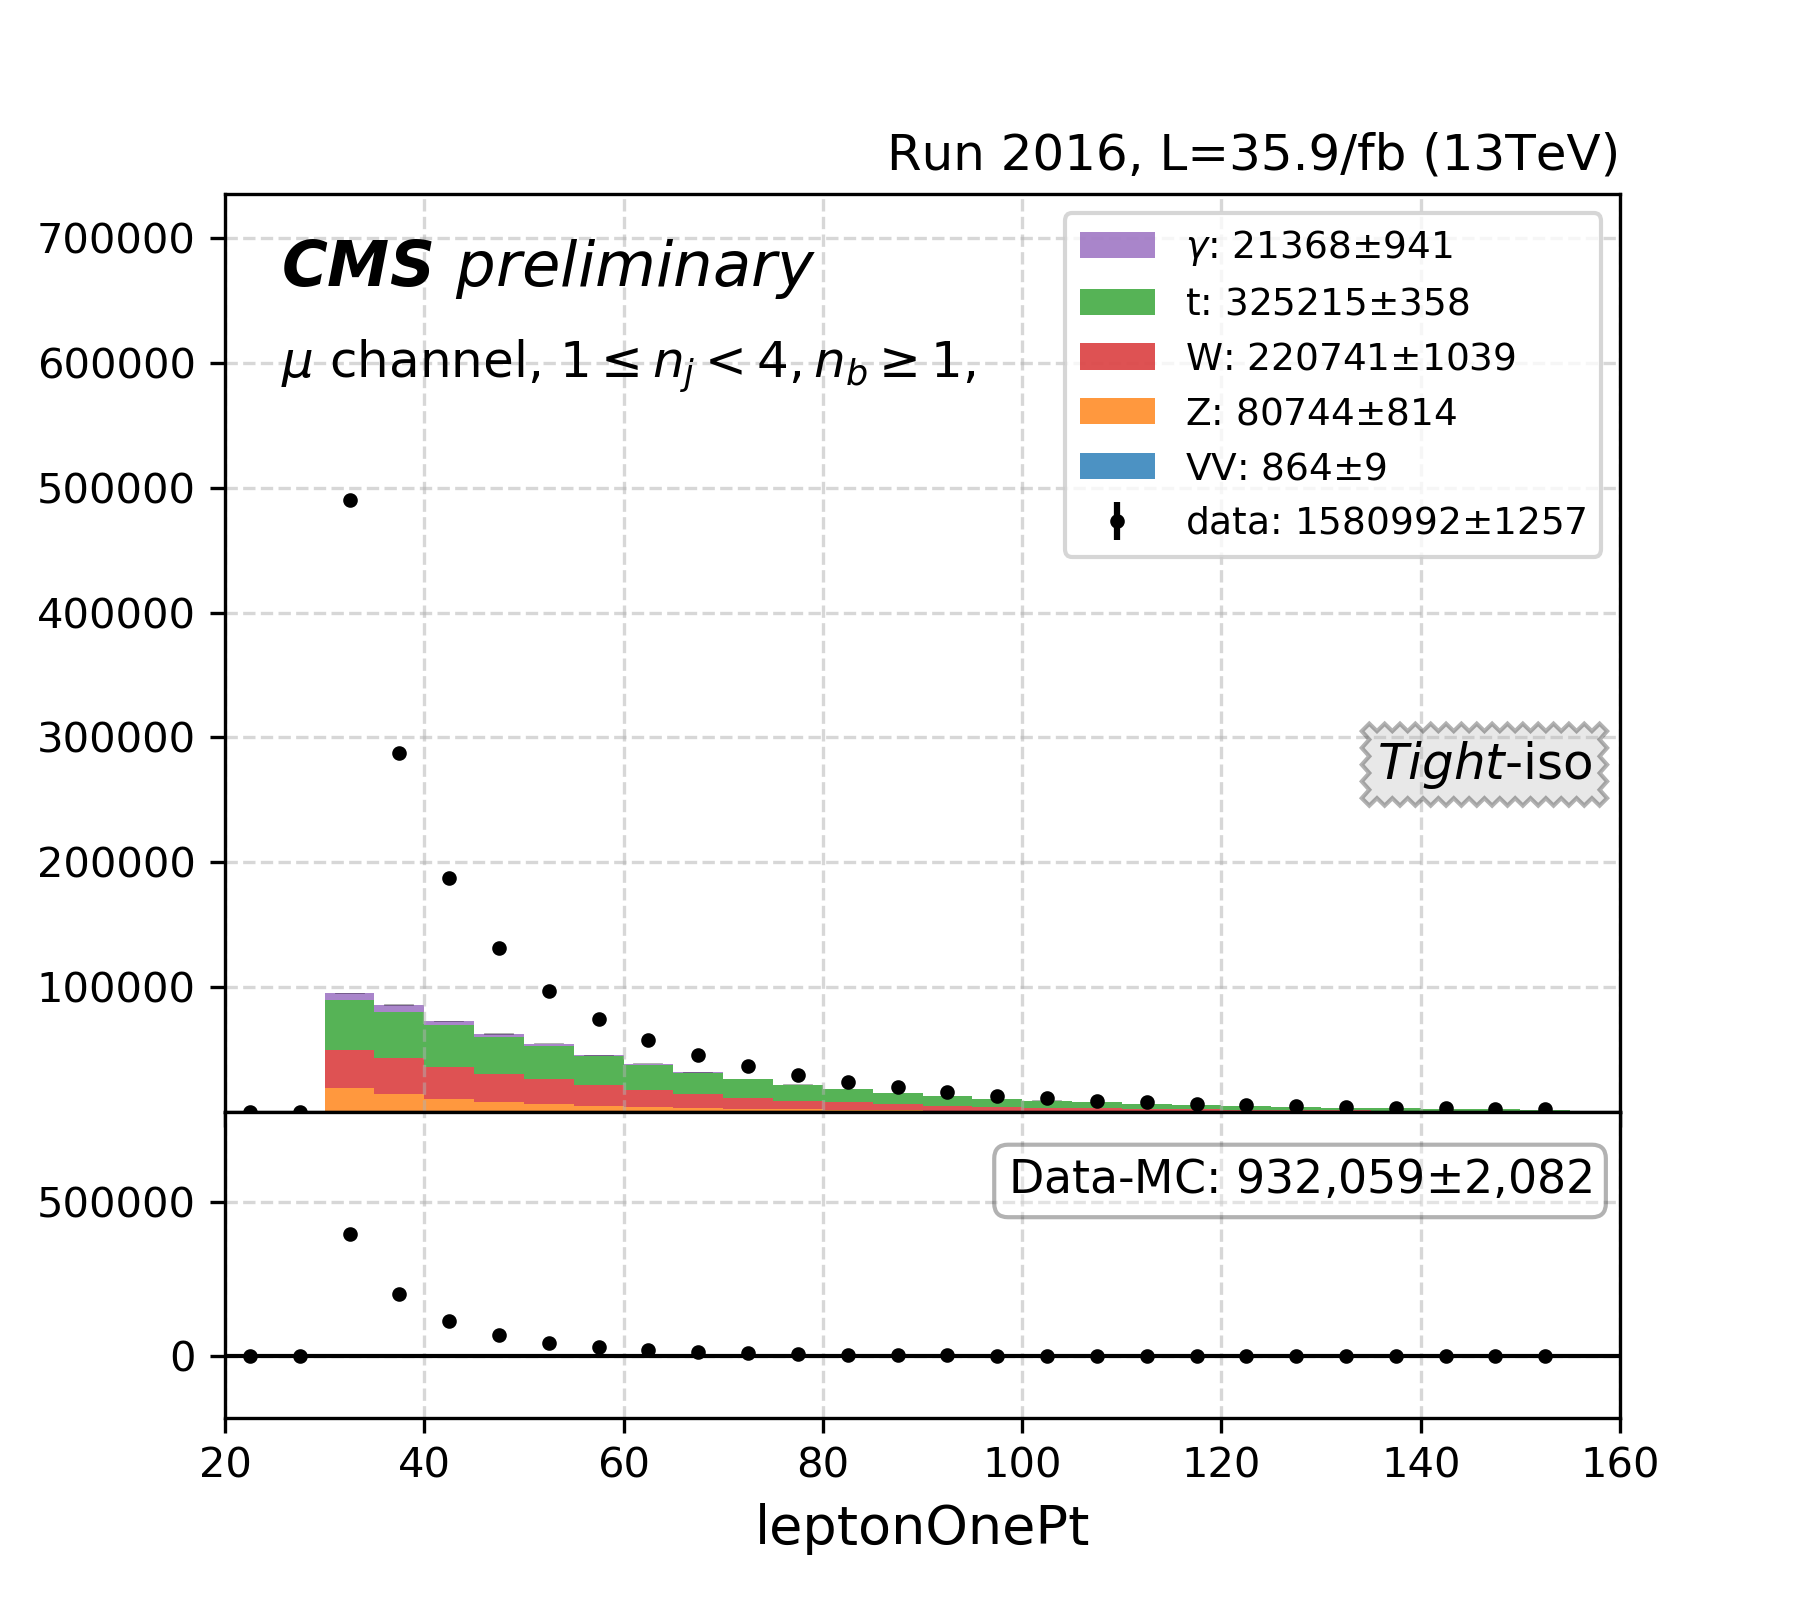
\includegraphics[width=0.24\textwidth]{appendices/qcdSF/figures/123j1b/mu_leptonOnePt_True.png}
    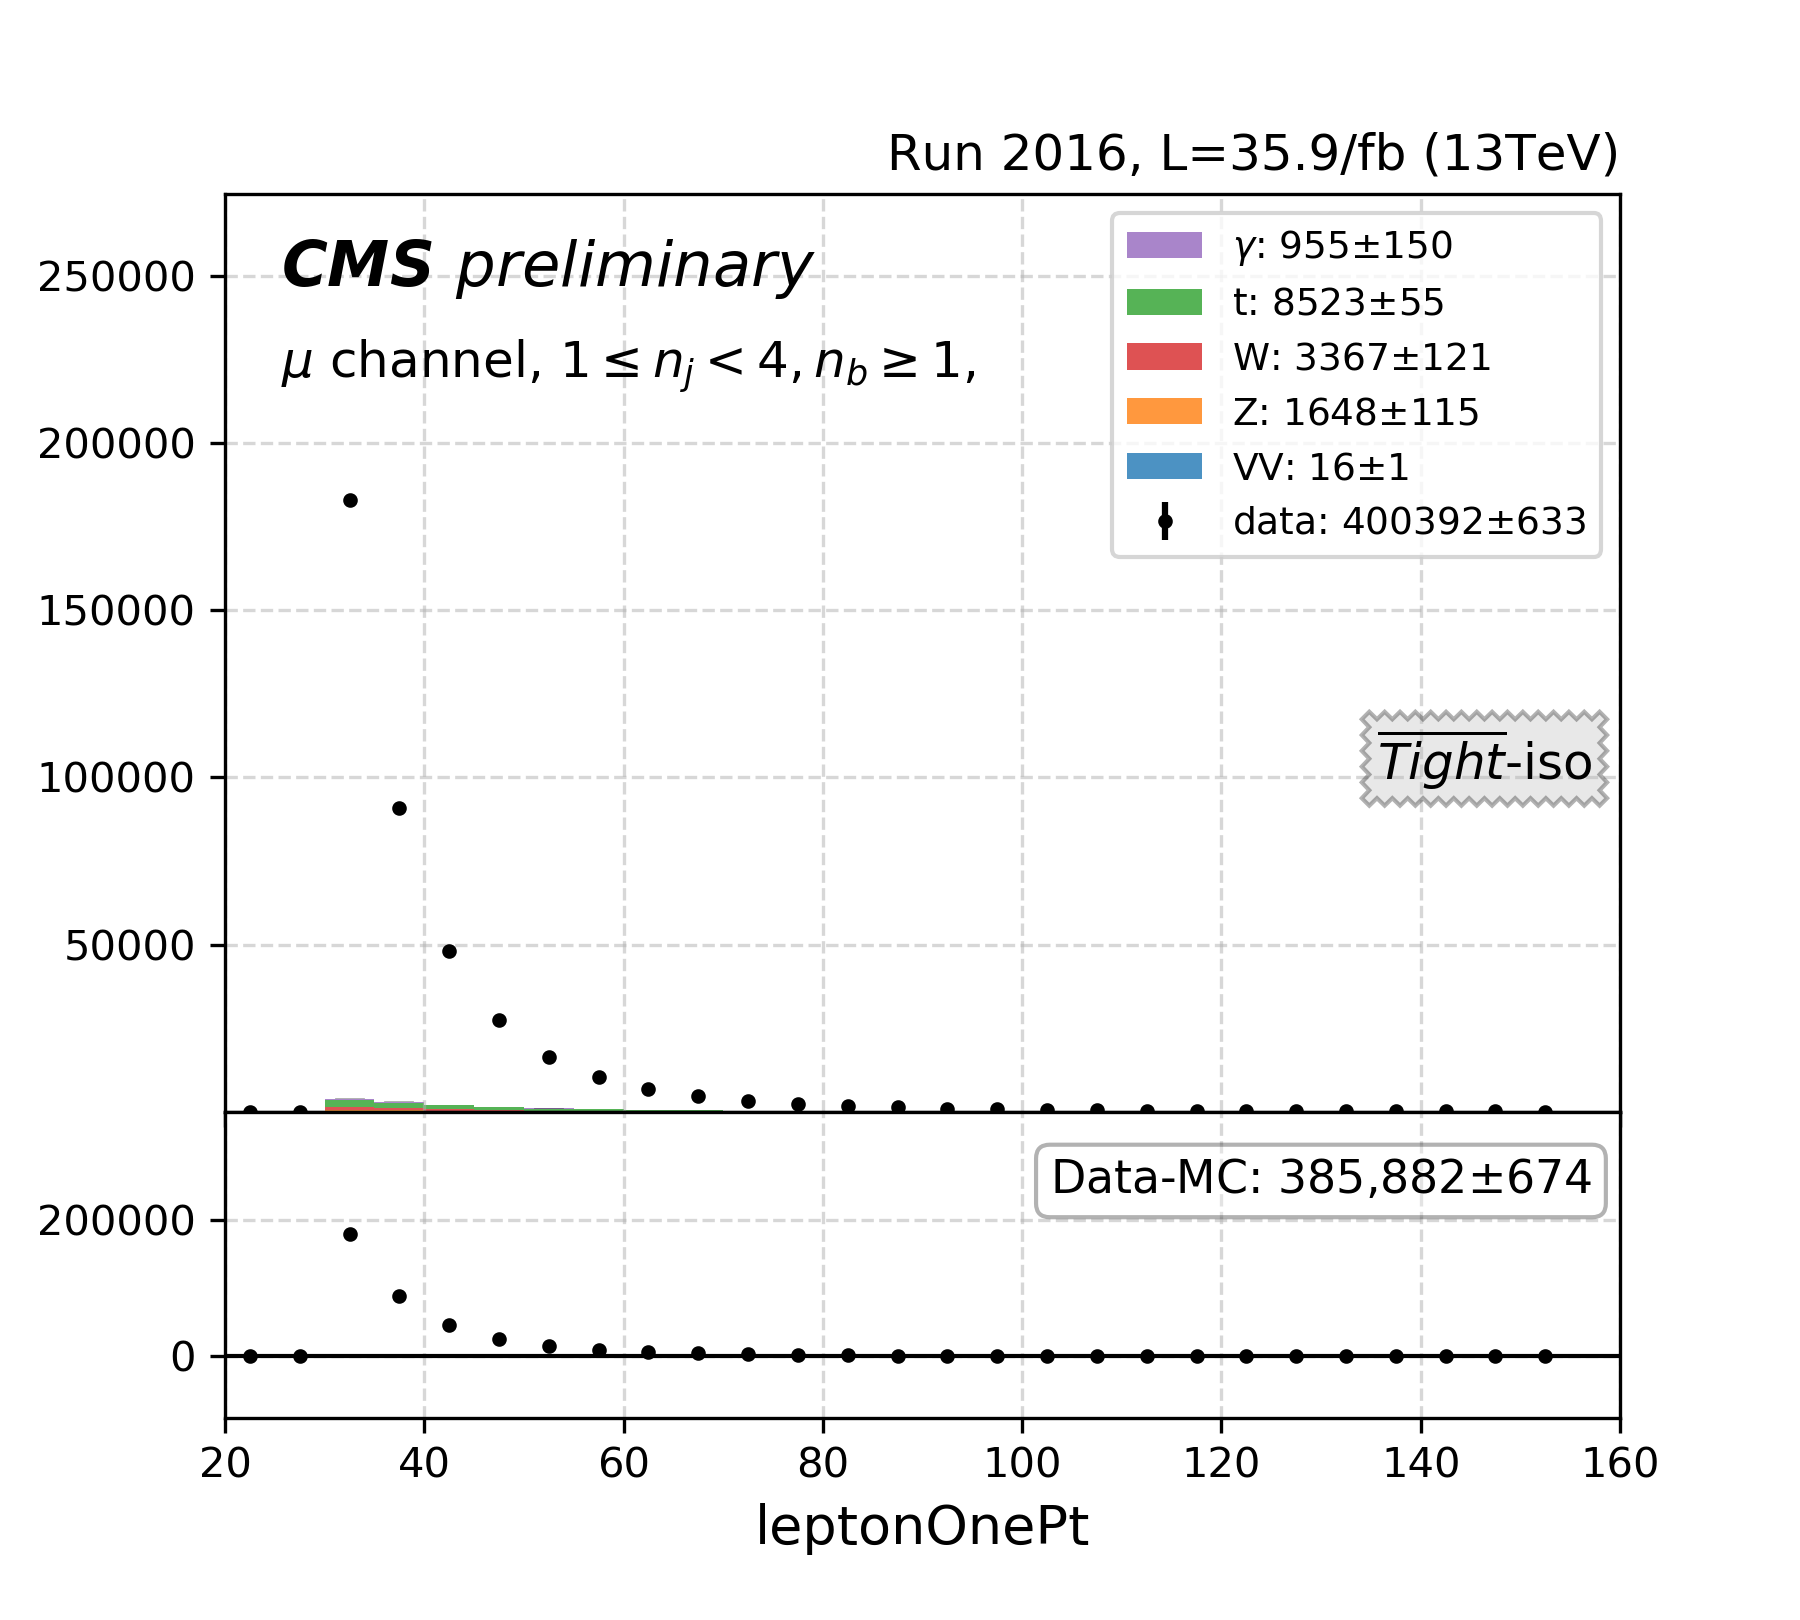
\includegraphics[width=0.24\textwidth]{appendices/qcdSF/figures/123j1b/mu_leptonOnePt_False.png}
    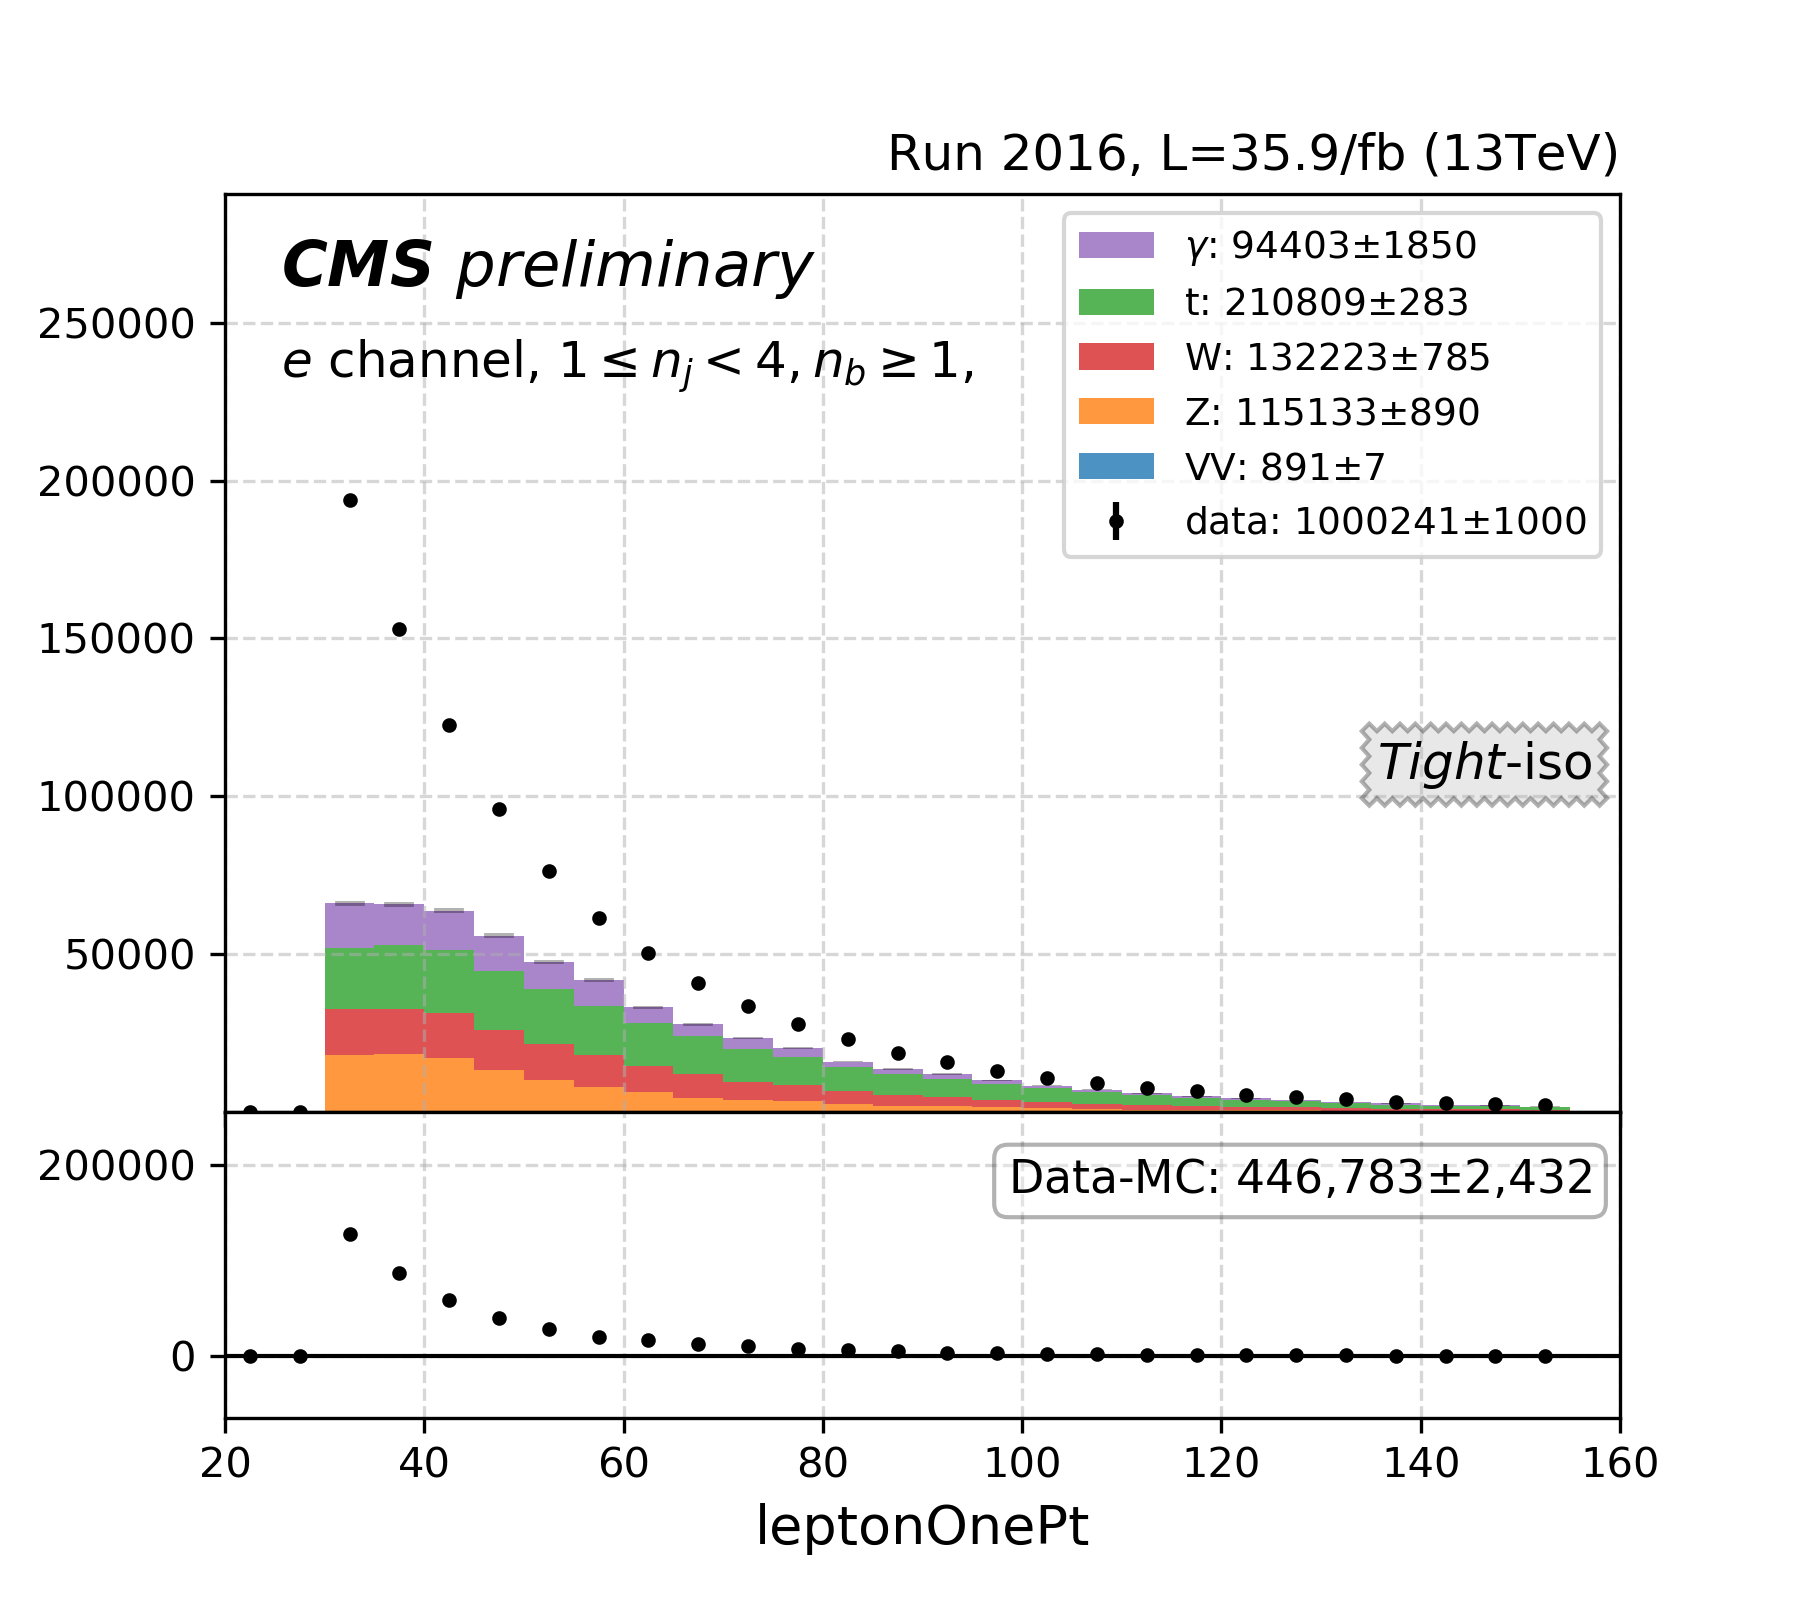
\includegraphics[width=0.24\textwidth]{appendices/qcdSF/figures/123j1b/e_leptonOnePt_True.png}
    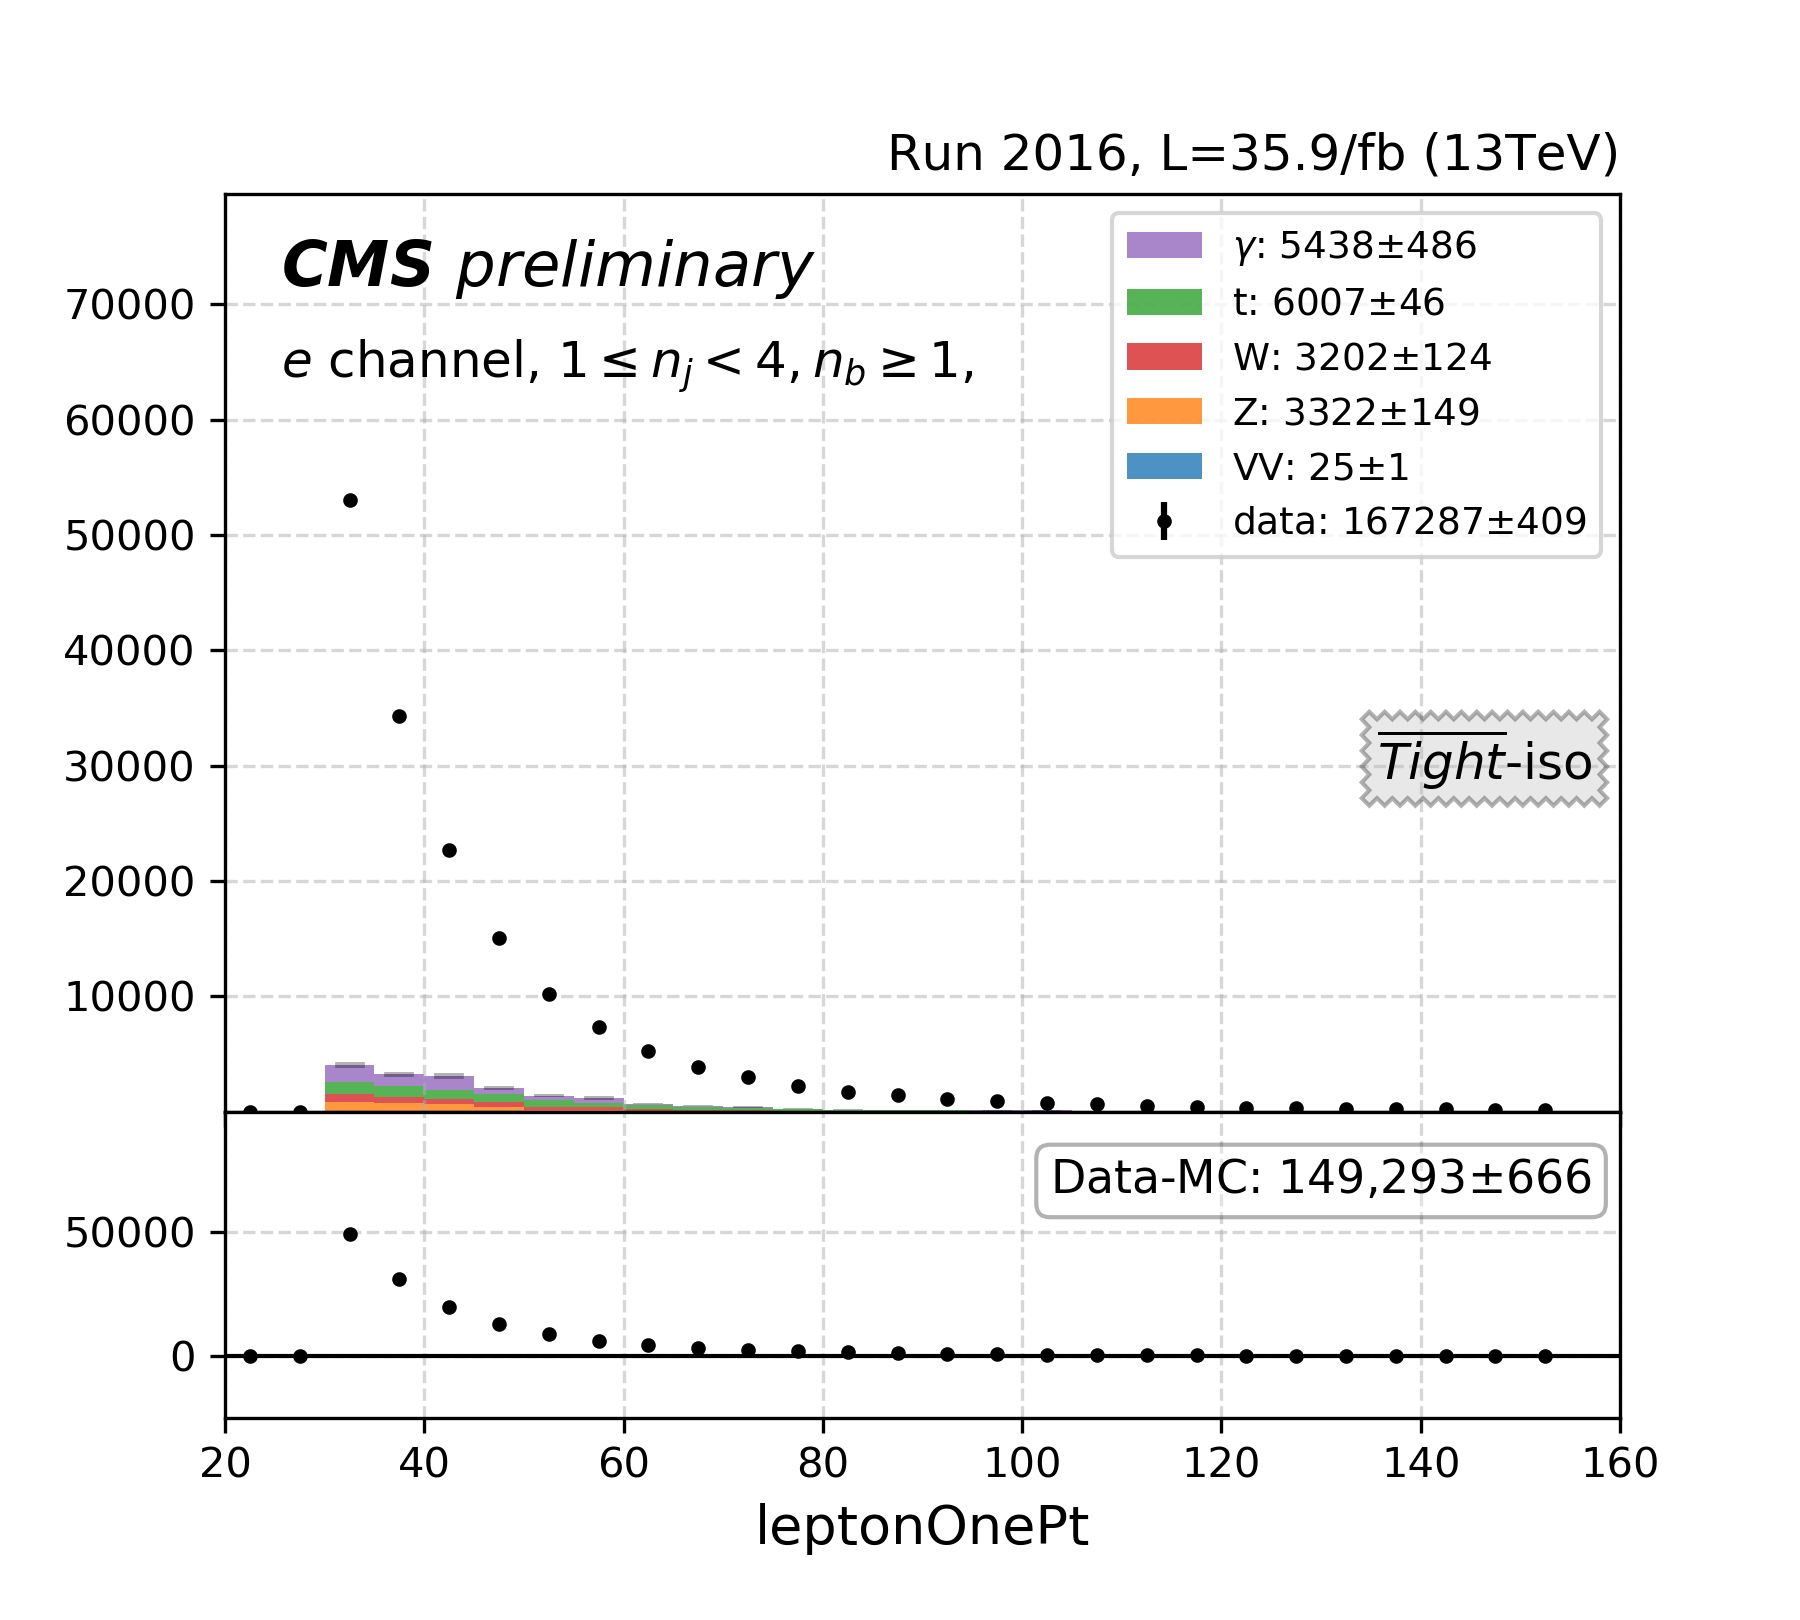
\includegraphics[width=0.24\textwidth]{appendices/qcdSF/figures/123j1b/e_leptonOnePt_False.png}
    
    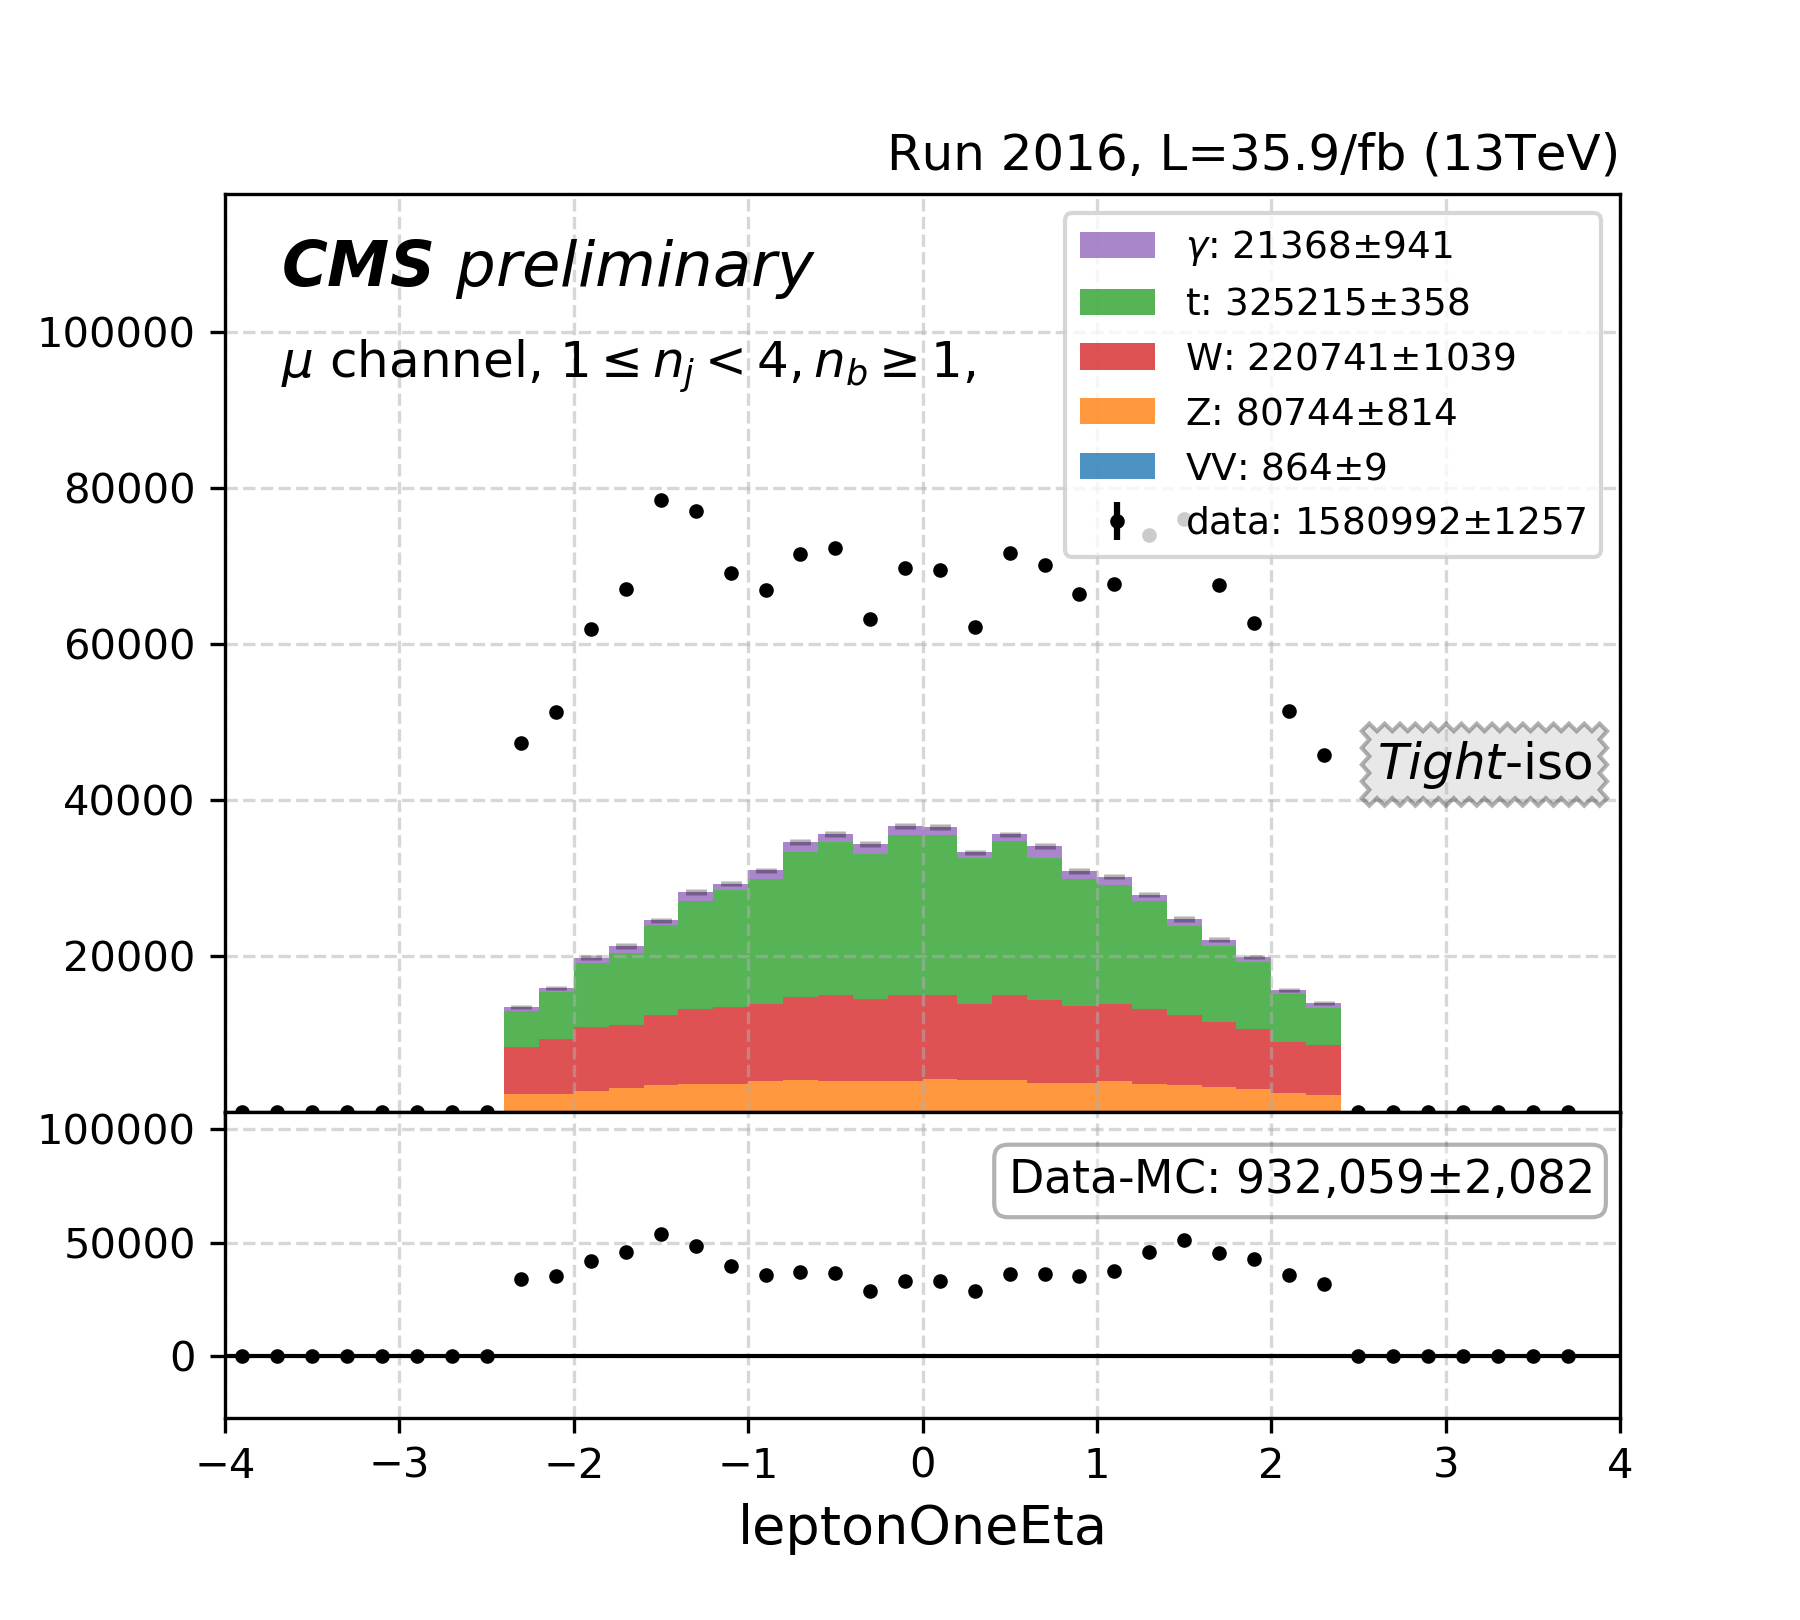
\includegraphics[width=0.24\textwidth]{appendices/qcdSF/figures/123j1b/mu_leptonOneEta_True.png}
    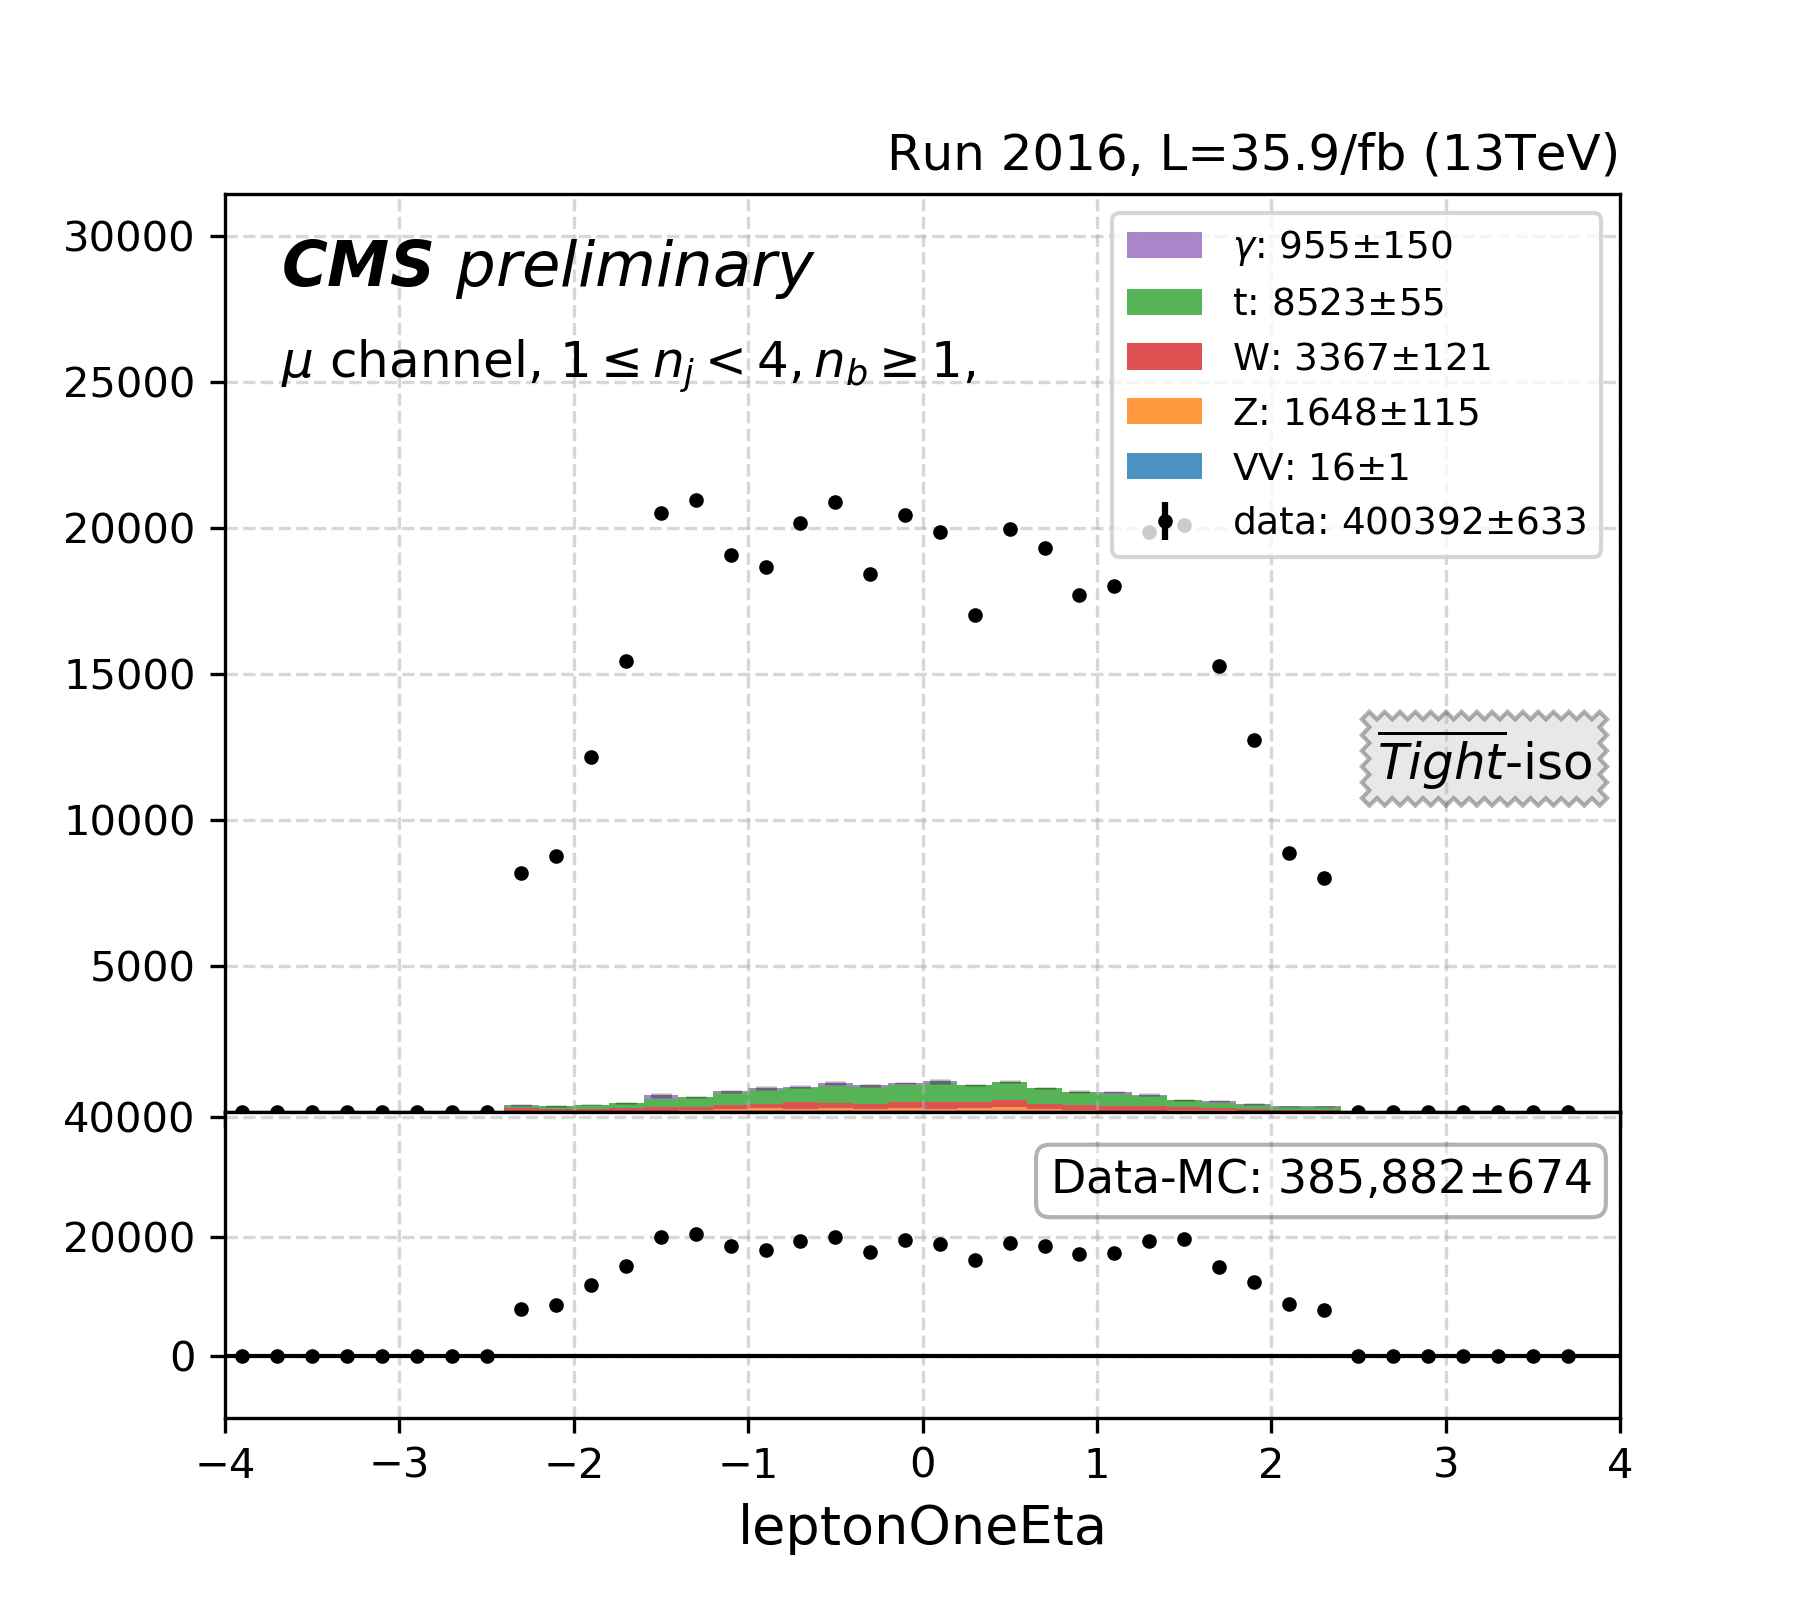
\includegraphics[width=0.24\textwidth]{appendices/qcdSF/figures/123j1b/mu_leptonOneEta_False.png}
    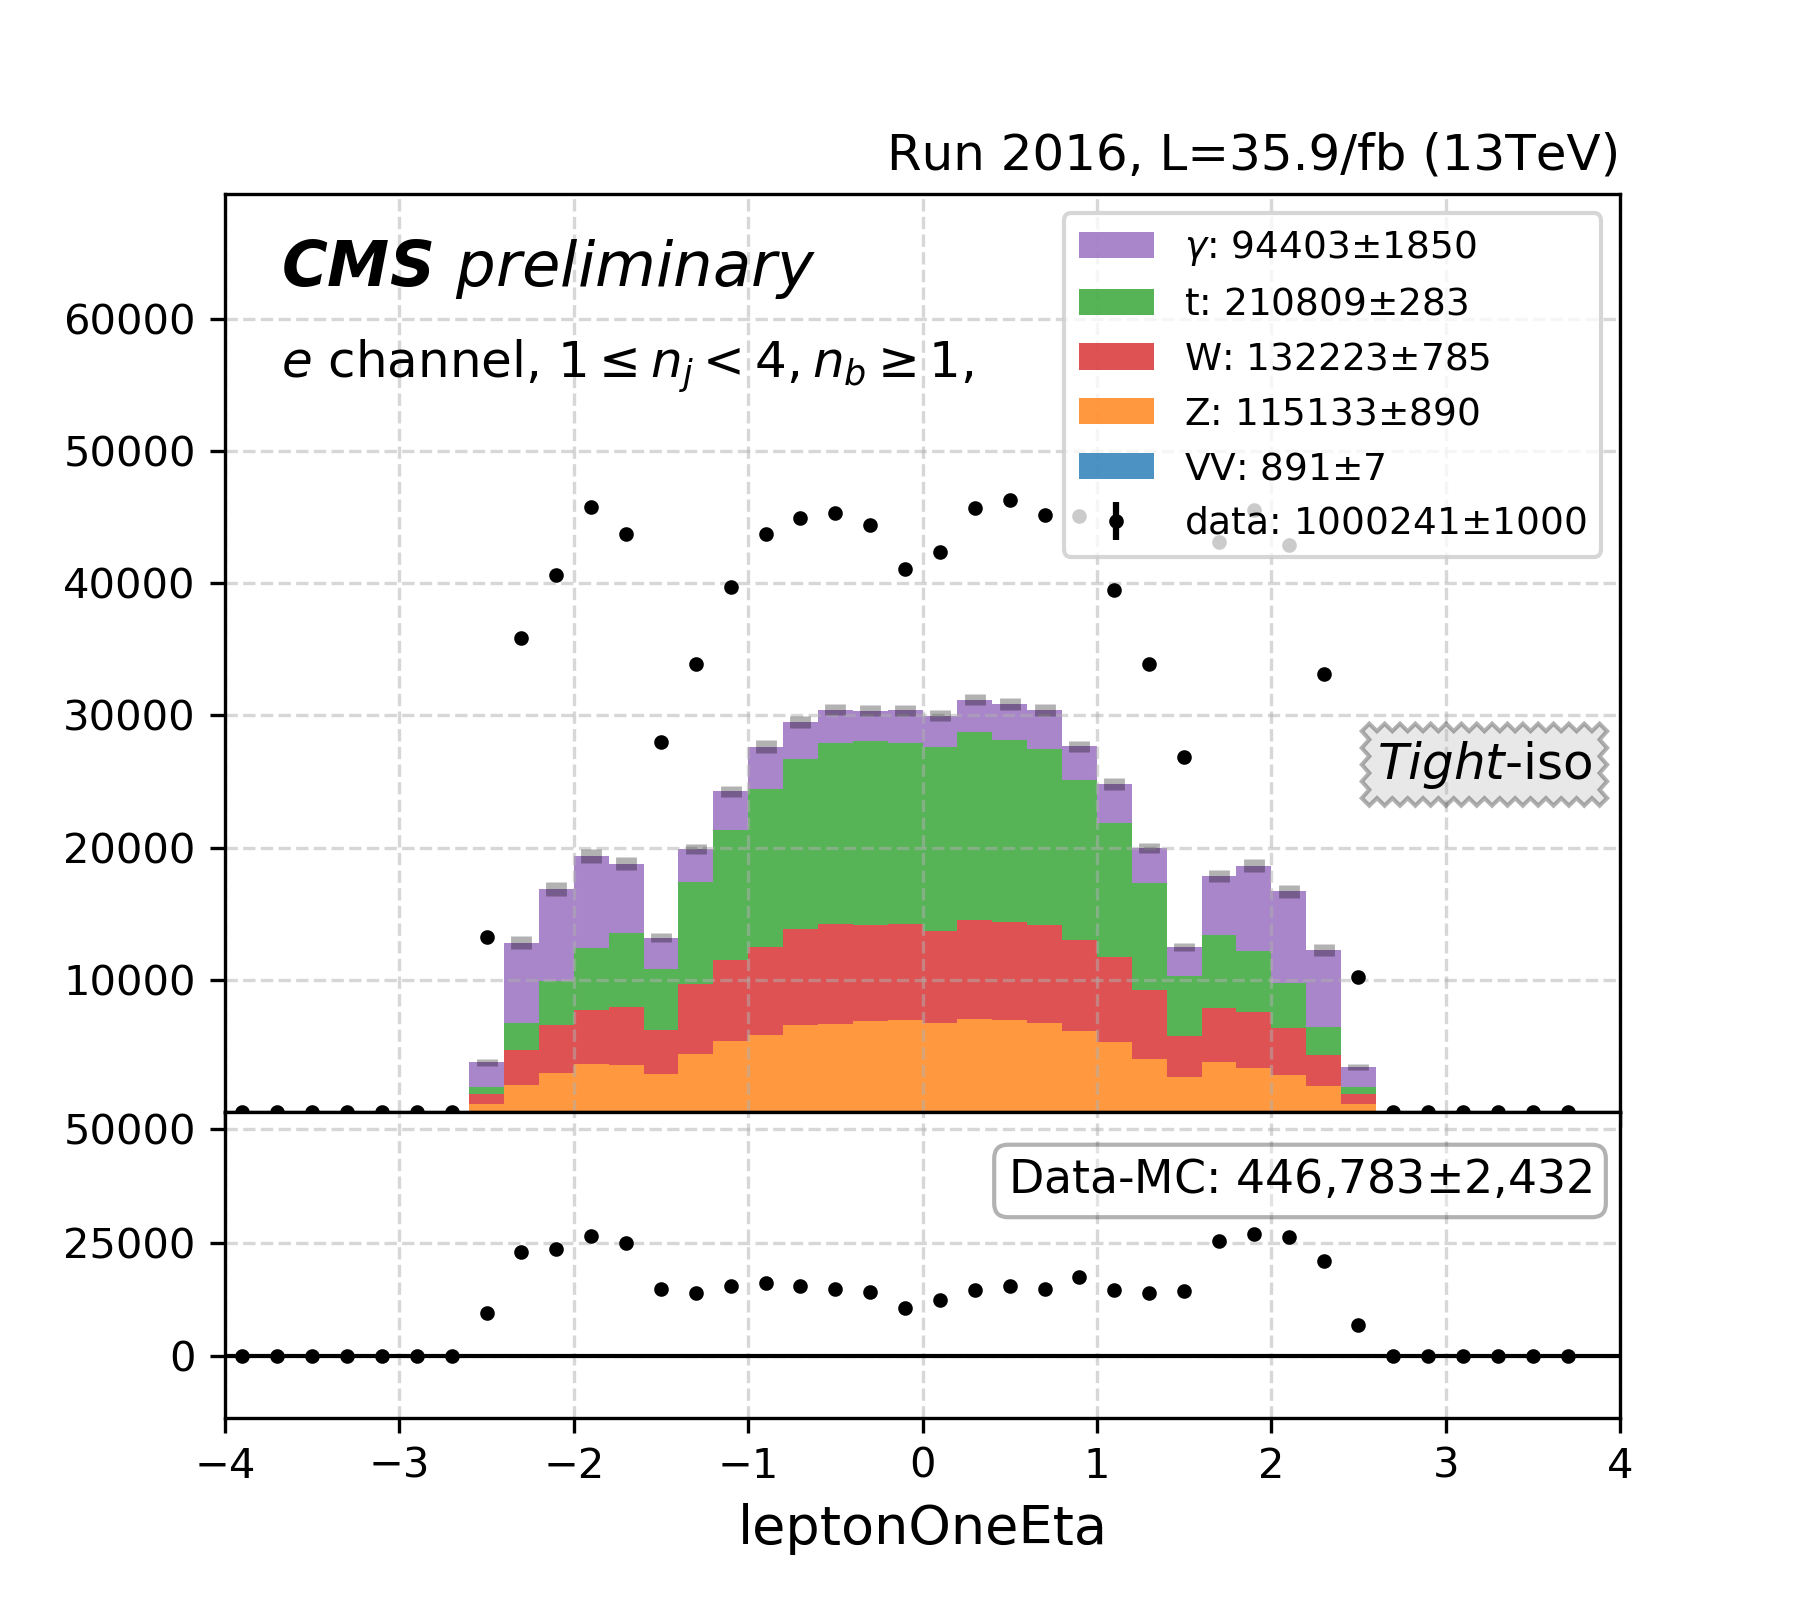
\includegraphics[width=0.24\textwidth]{appendices/qcdSF/figures/123j1b/e_leptonOneEta_True.png}
    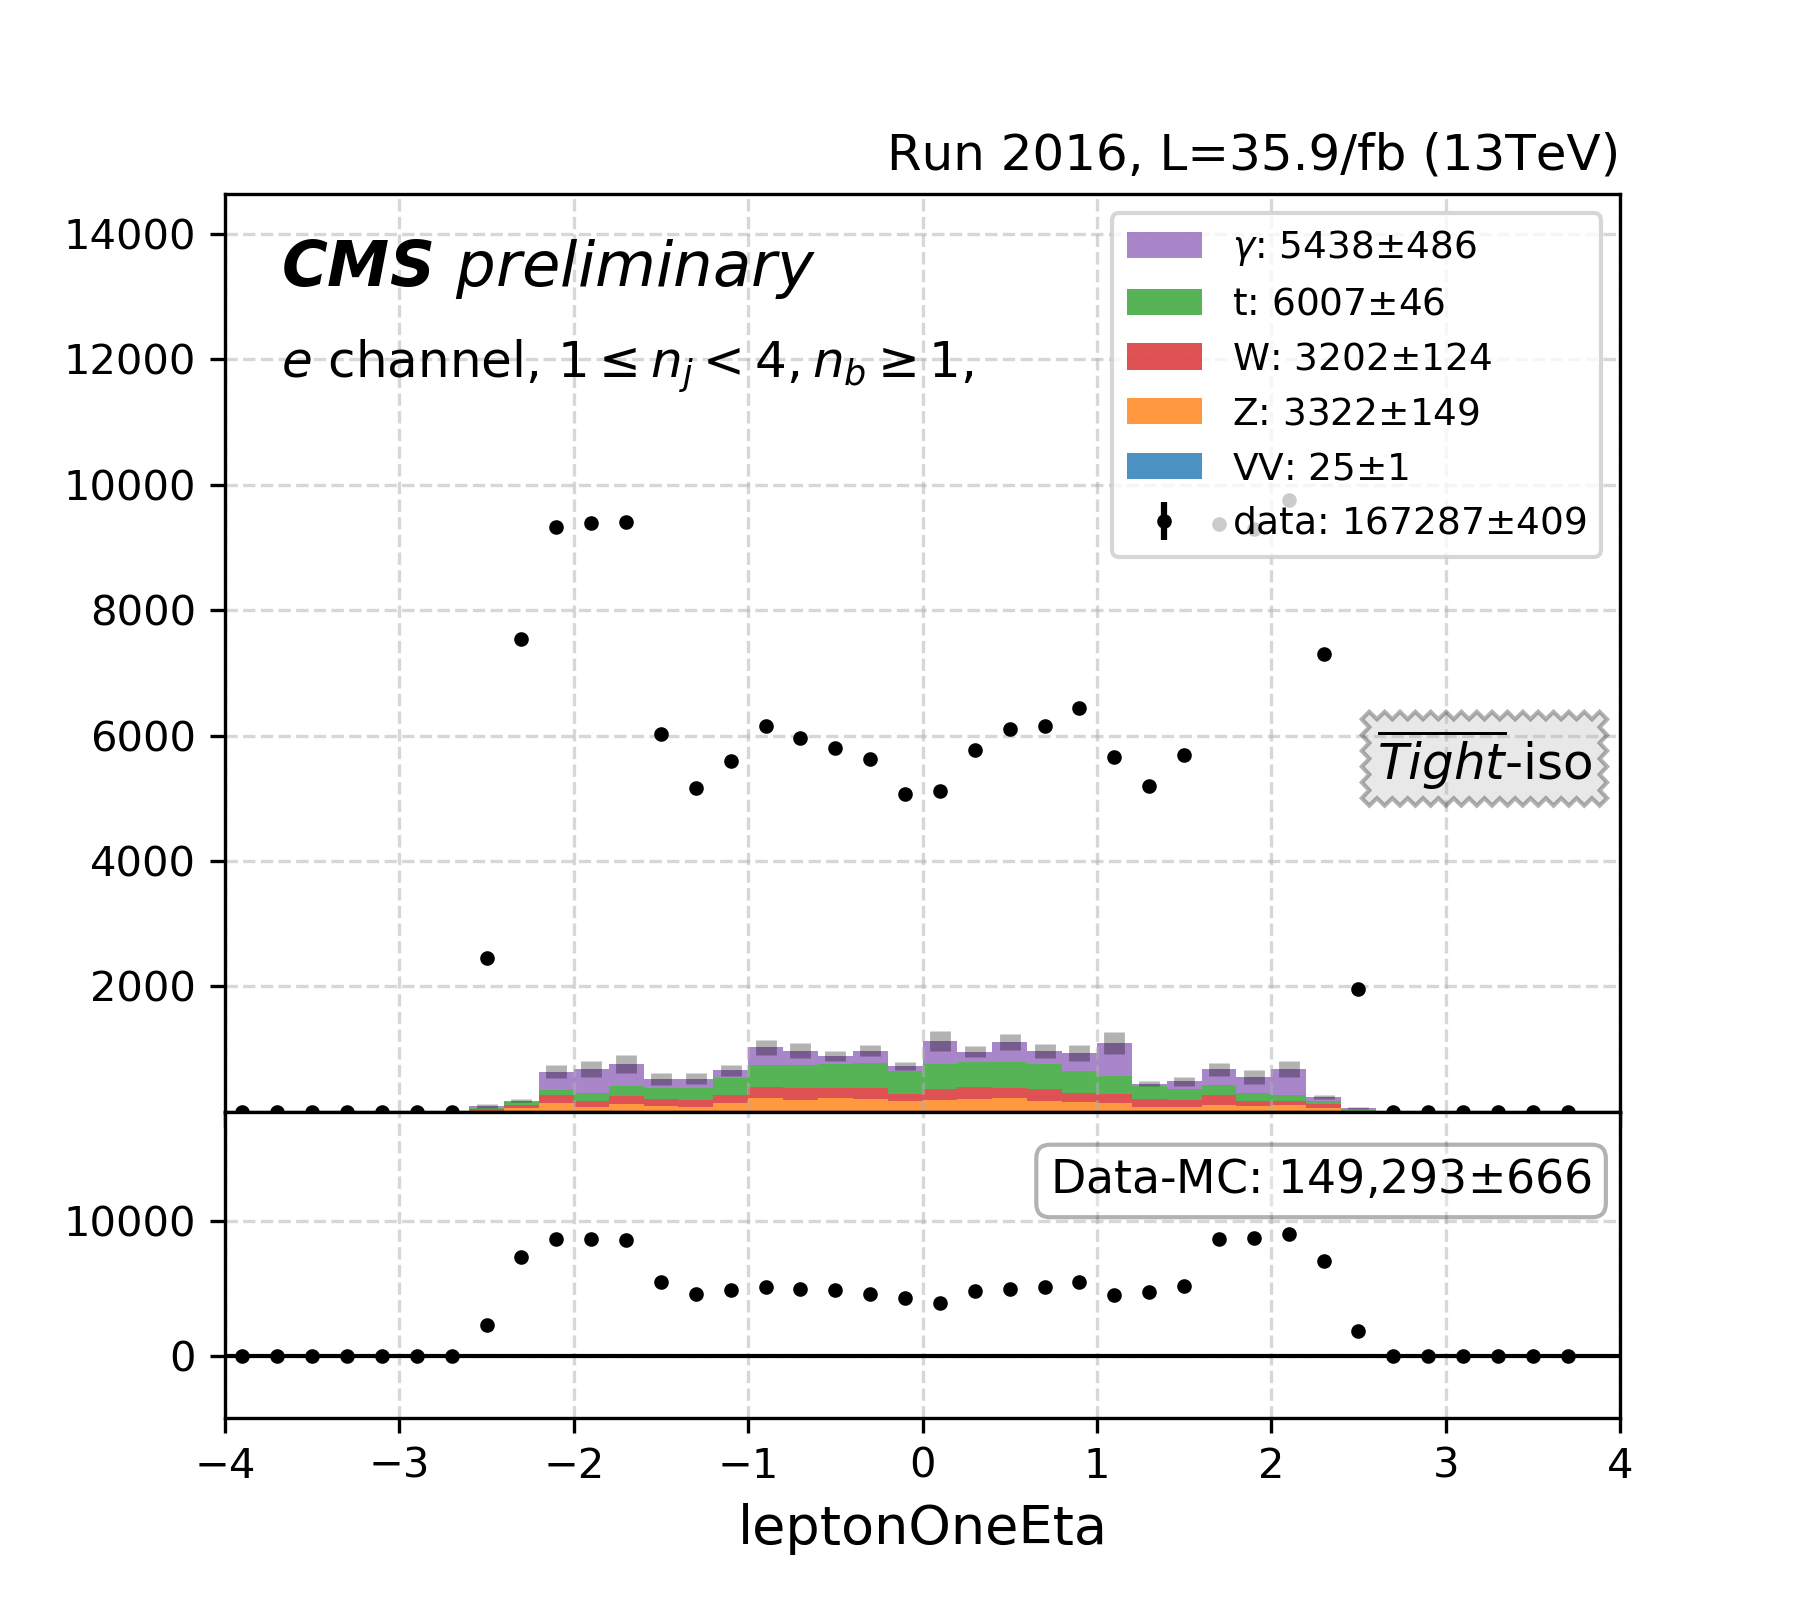
\includegraphics[width=0.24\textwidth]{appendices/qcdSF/figures/123j1b/e_leptonOneEta_False.png}
    
    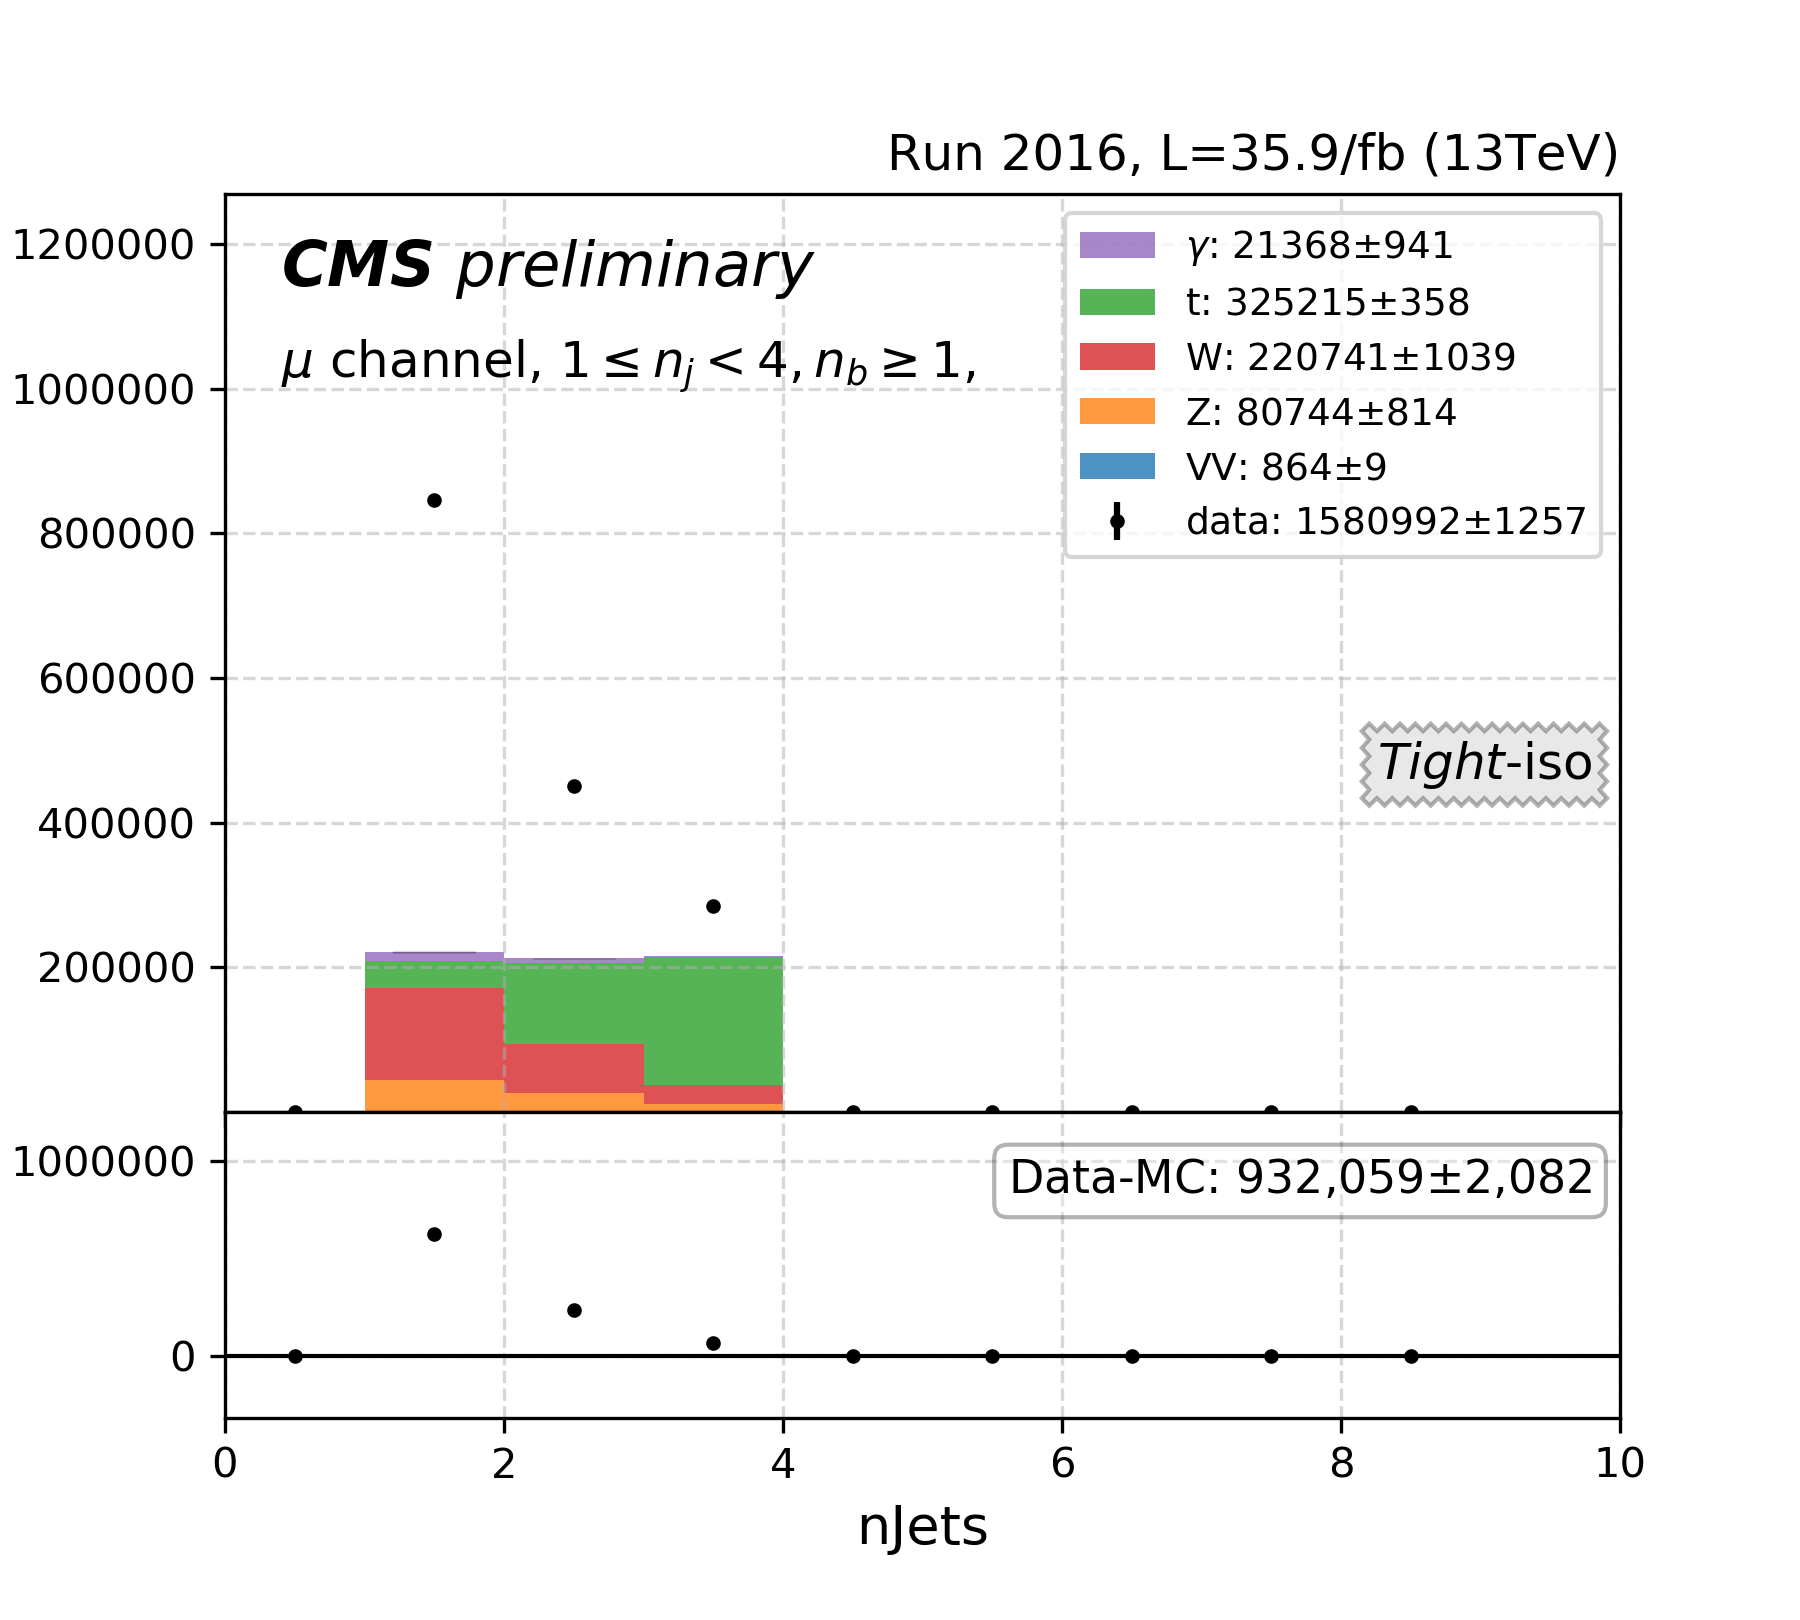
\includegraphics[width=0.24\textwidth]{appendices/qcdSF/figures/123j1b/mu_nJets_True.png}
    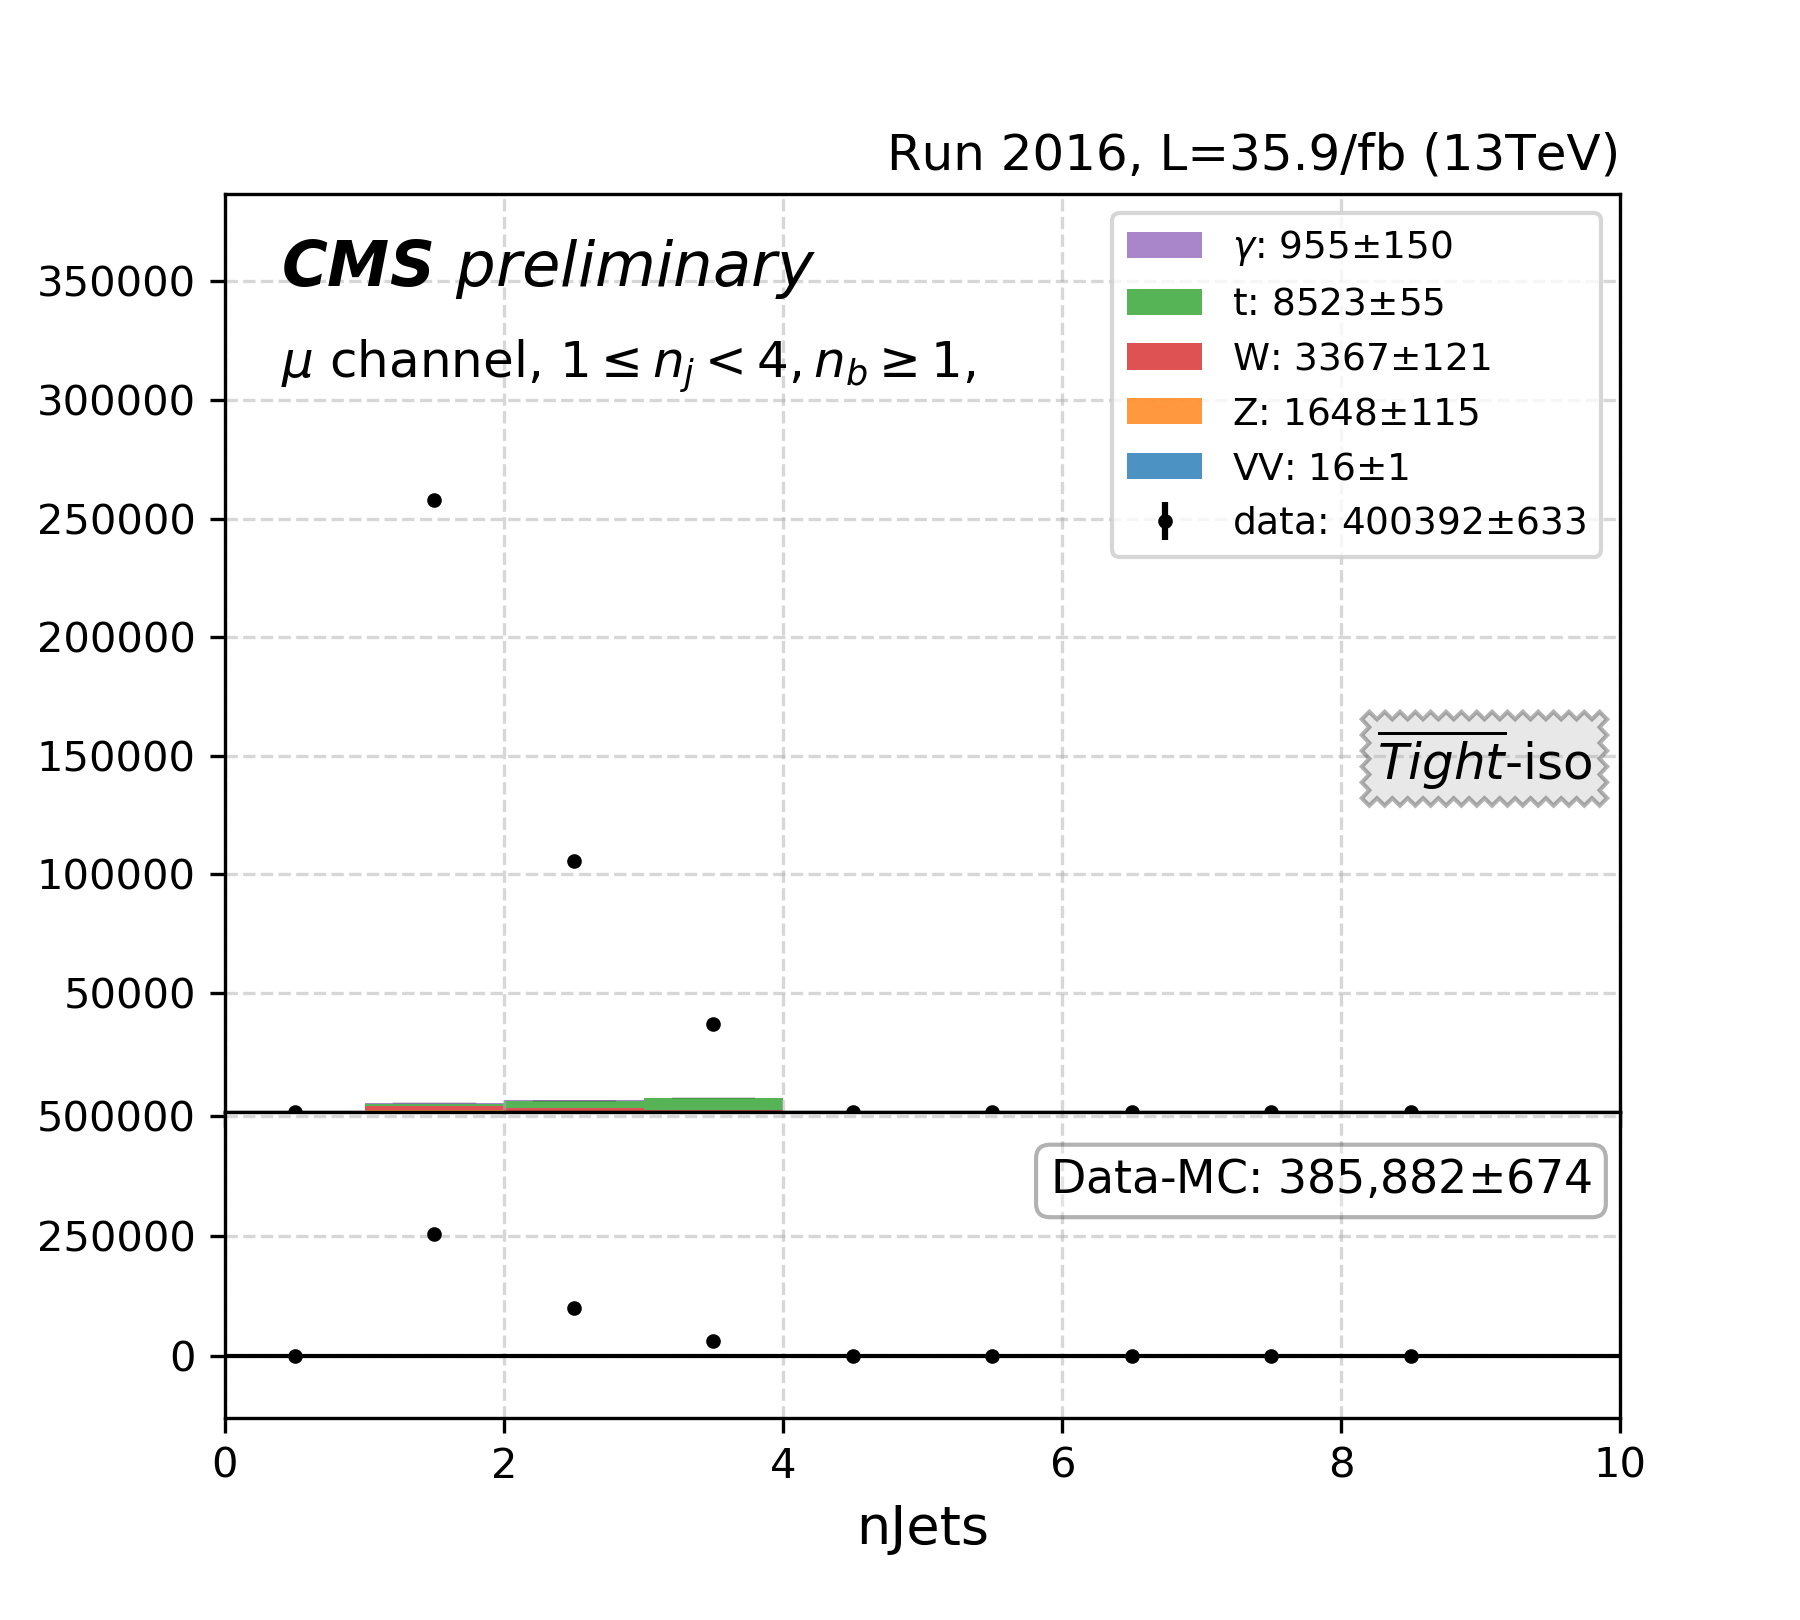
\includegraphics[width=0.24\textwidth]{appendices/qcdSF/figures/123j1b/mu_nJets_False.png}
    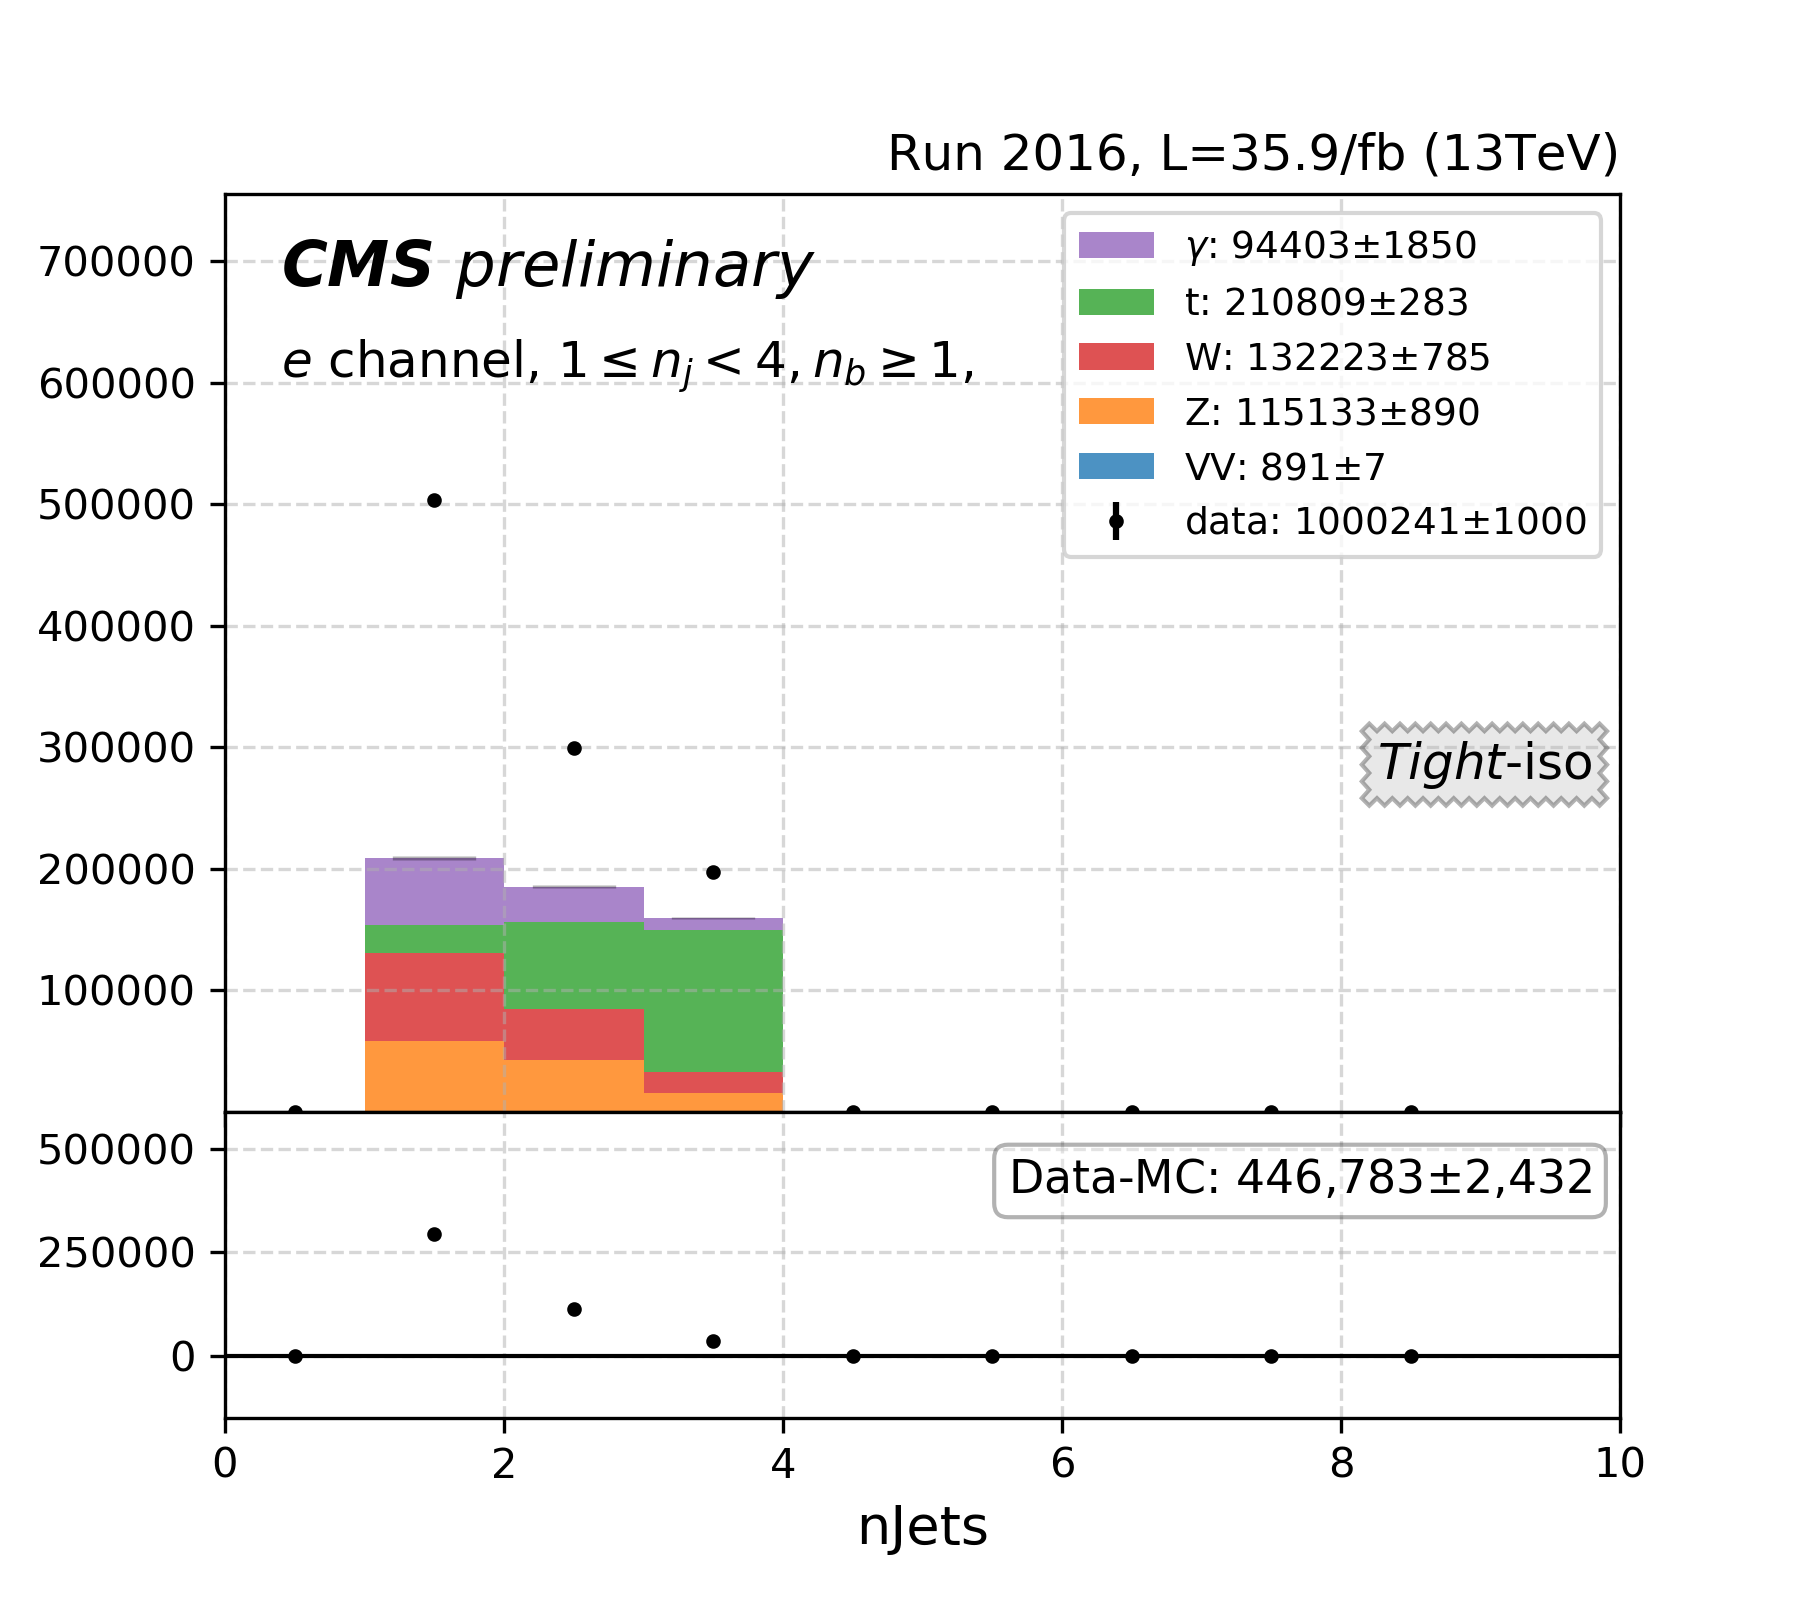
\includegraphics[width=0.24\textwidth]{appendices/qcdSF/figures/123j1b/e_nJets_True.png}
    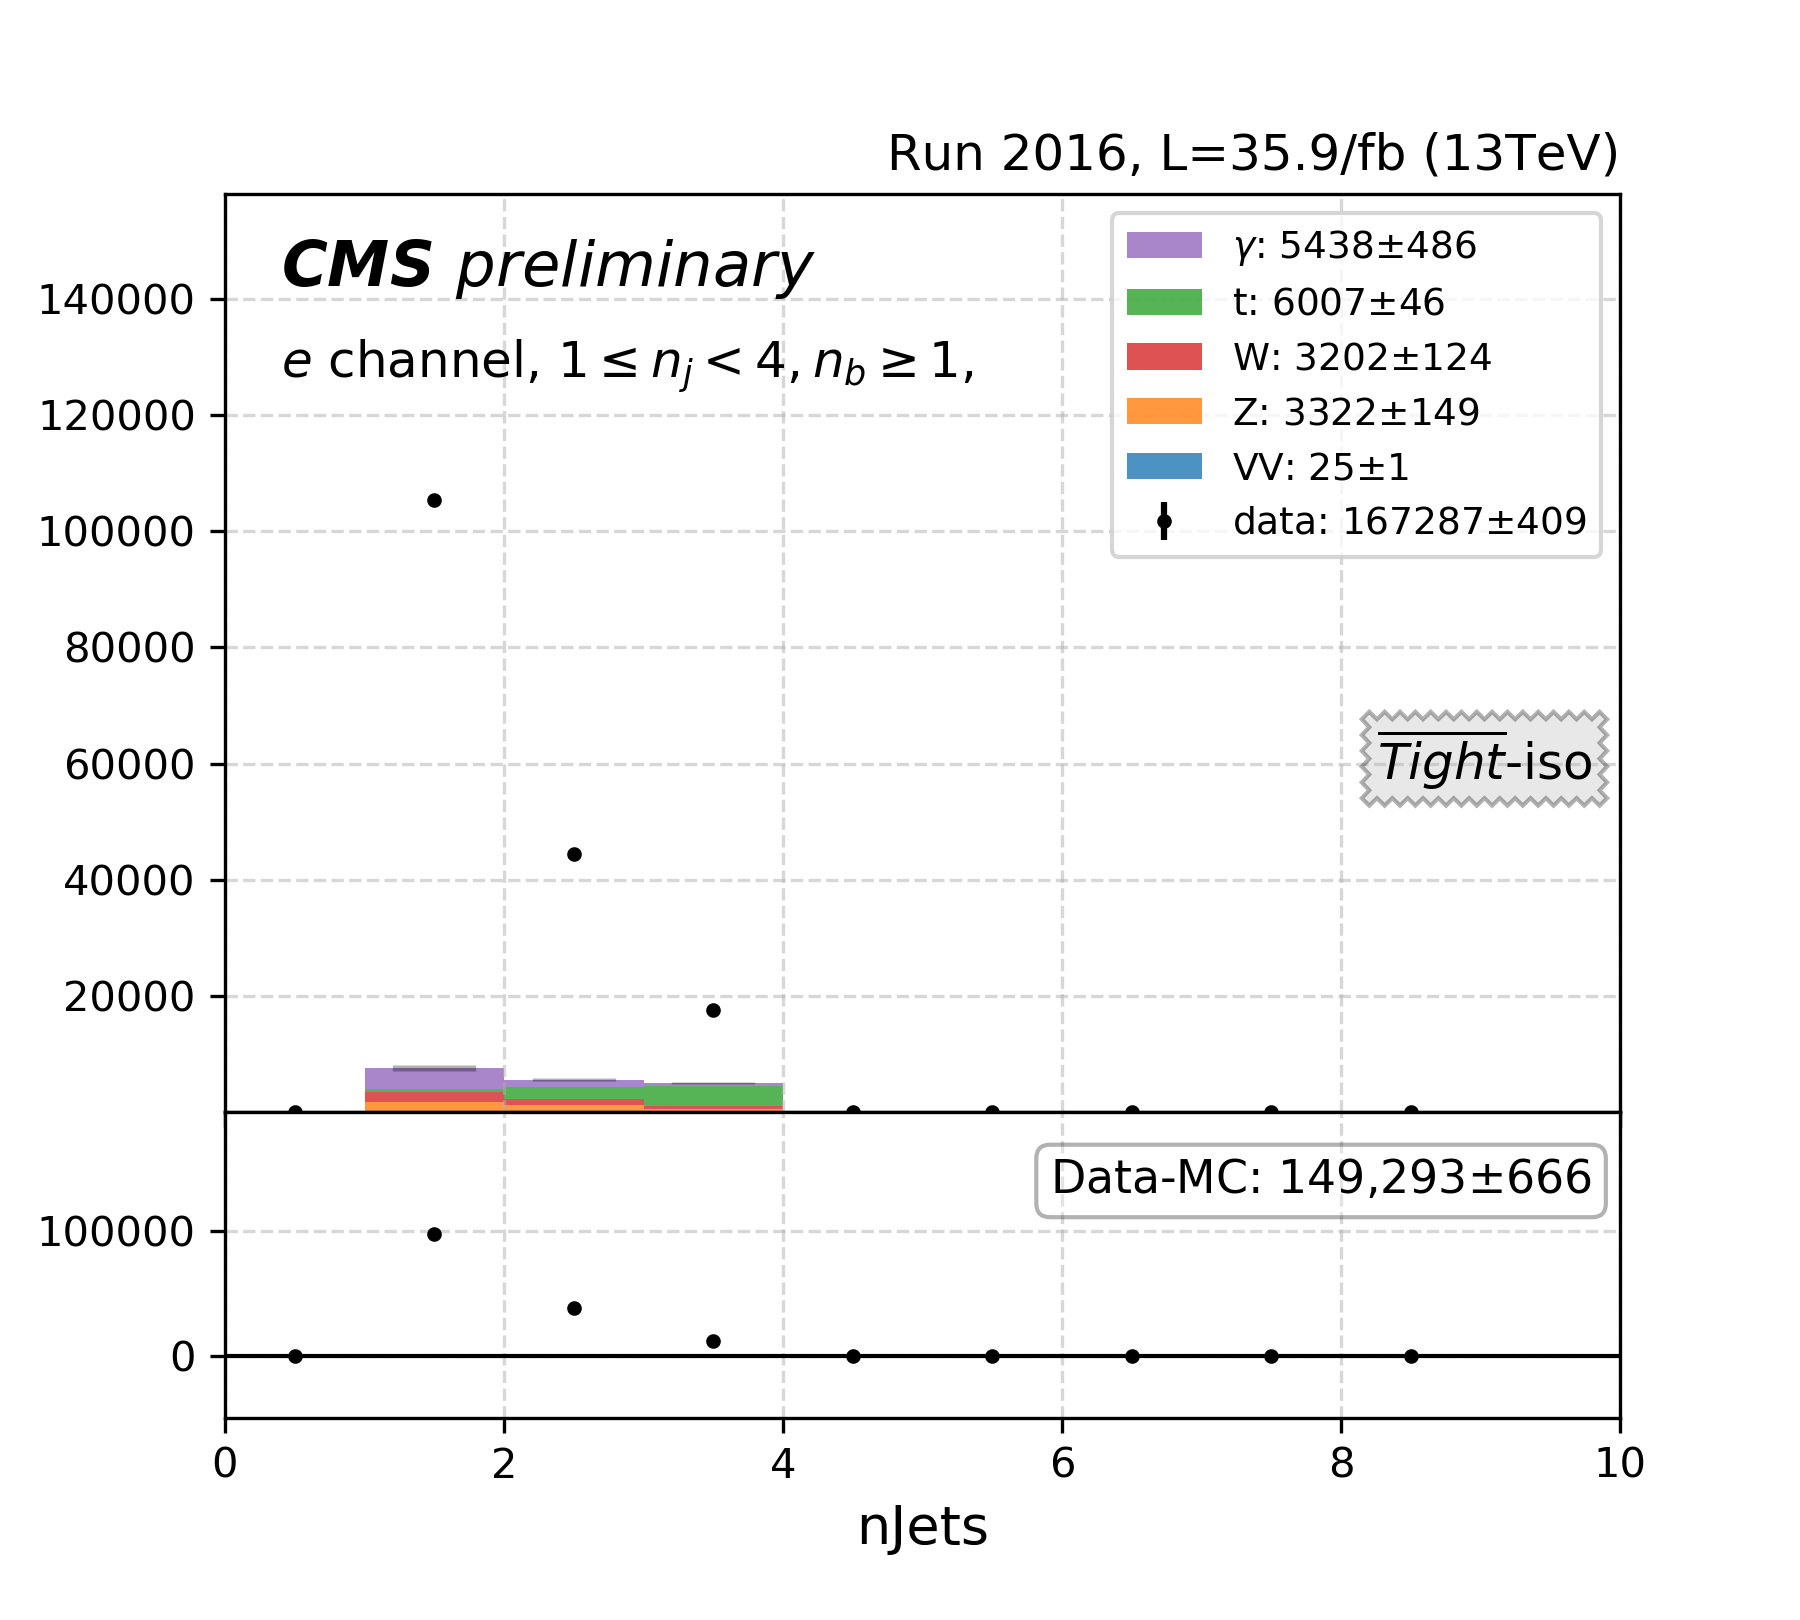
\includegraphics[width=0.24\textwidth]{appendices/qcdSF/figures/123j1b/e_nJets_False.png}
    
    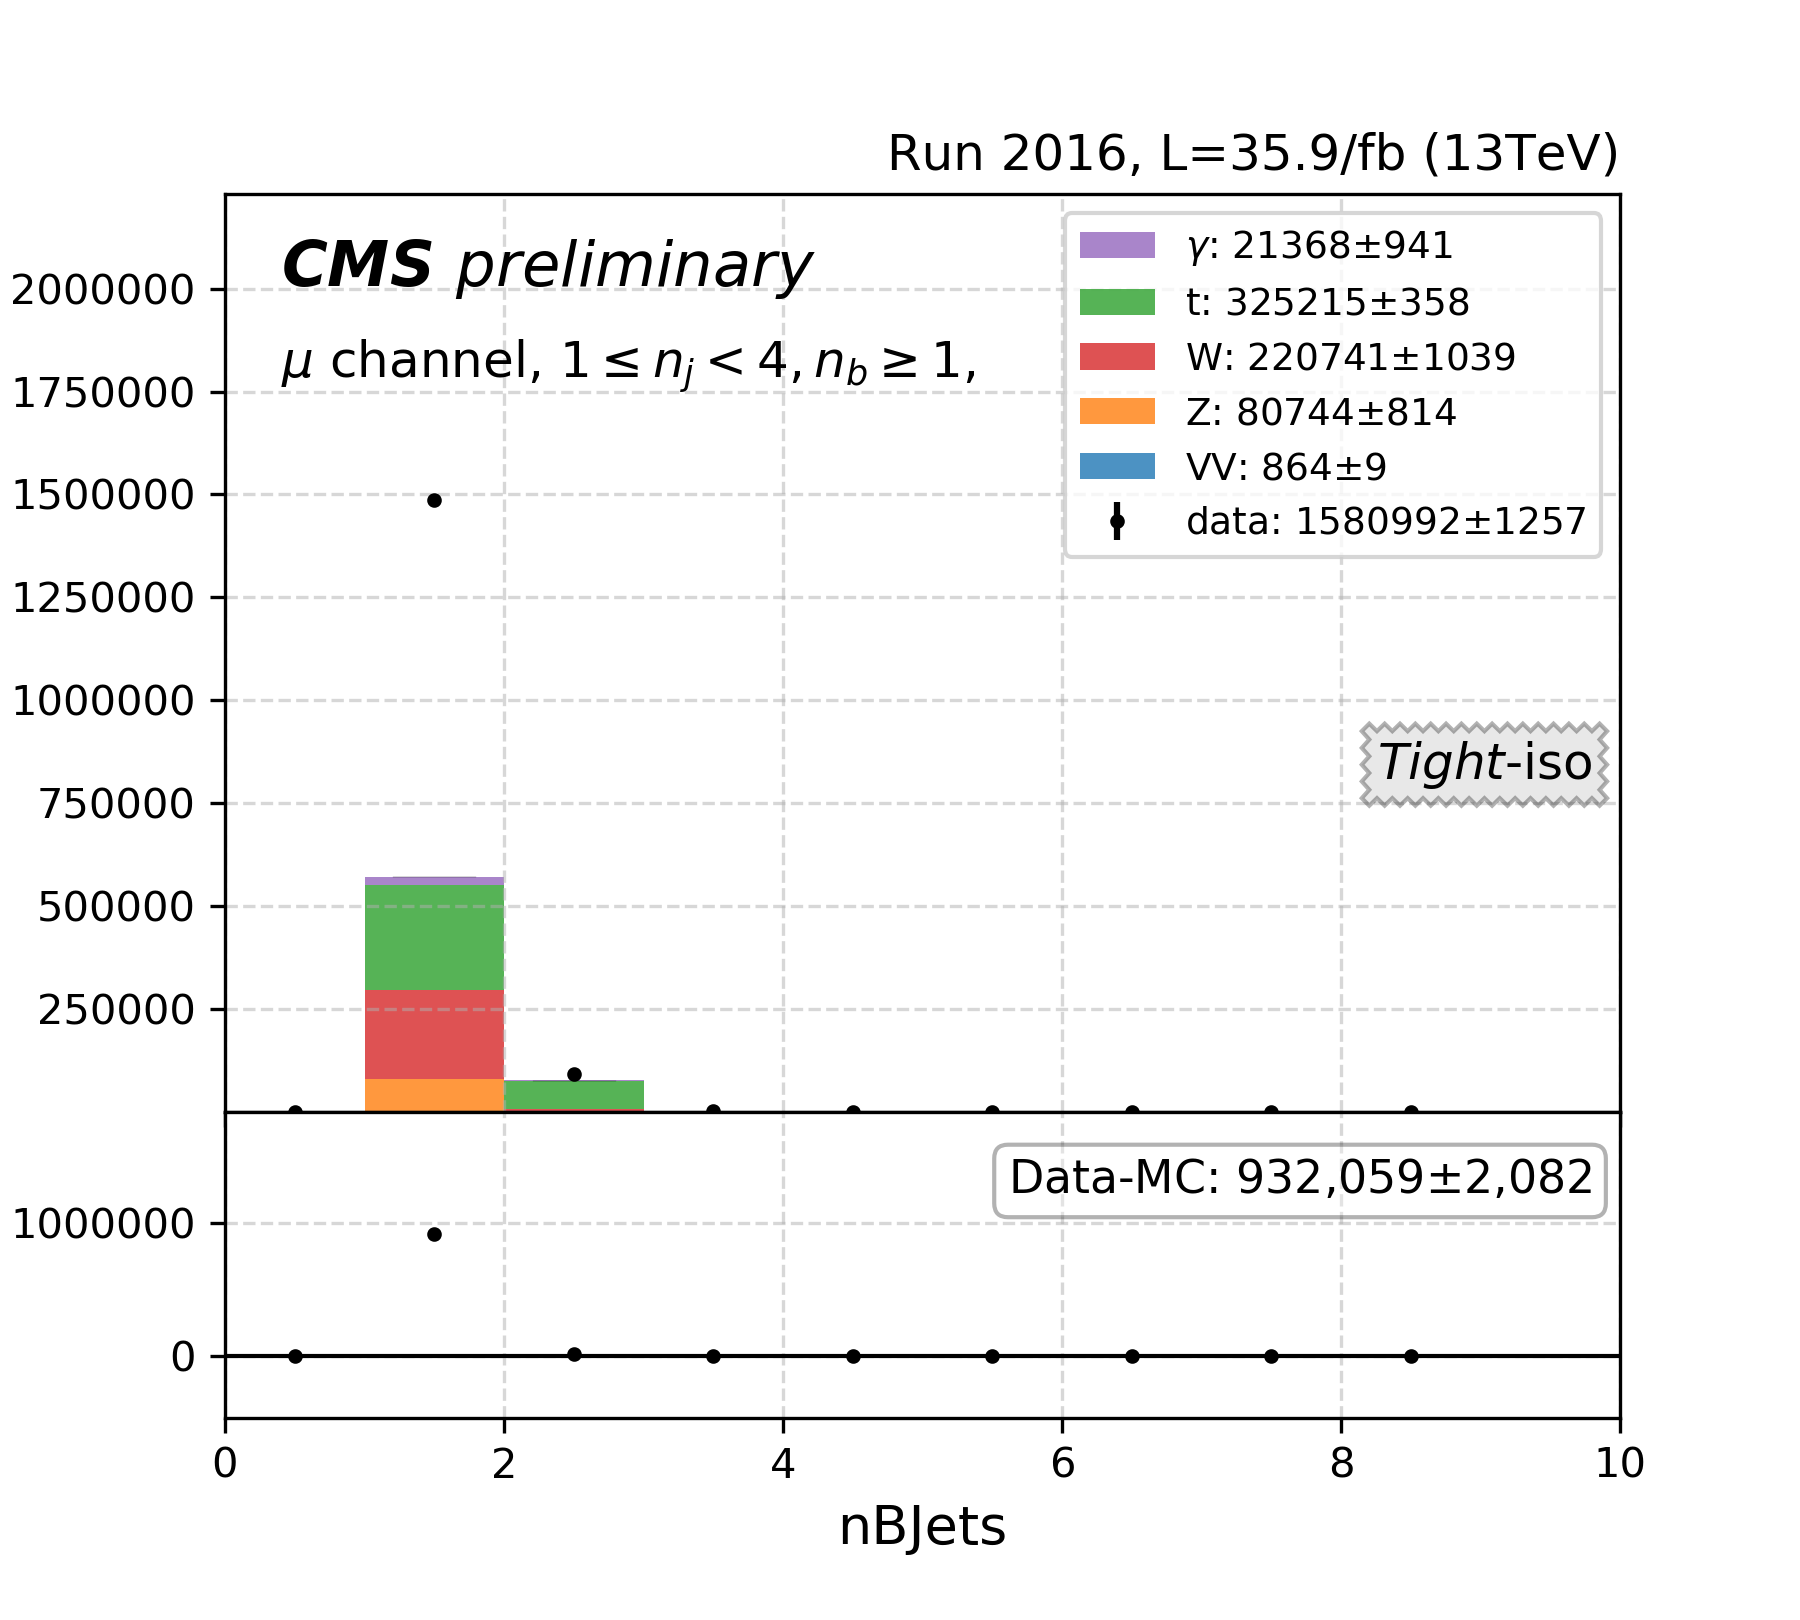
\includegraphics[width=0.24\textwidth]{appendices/qcdSF/figures/123j1b/mu_nBJets_True.png}
    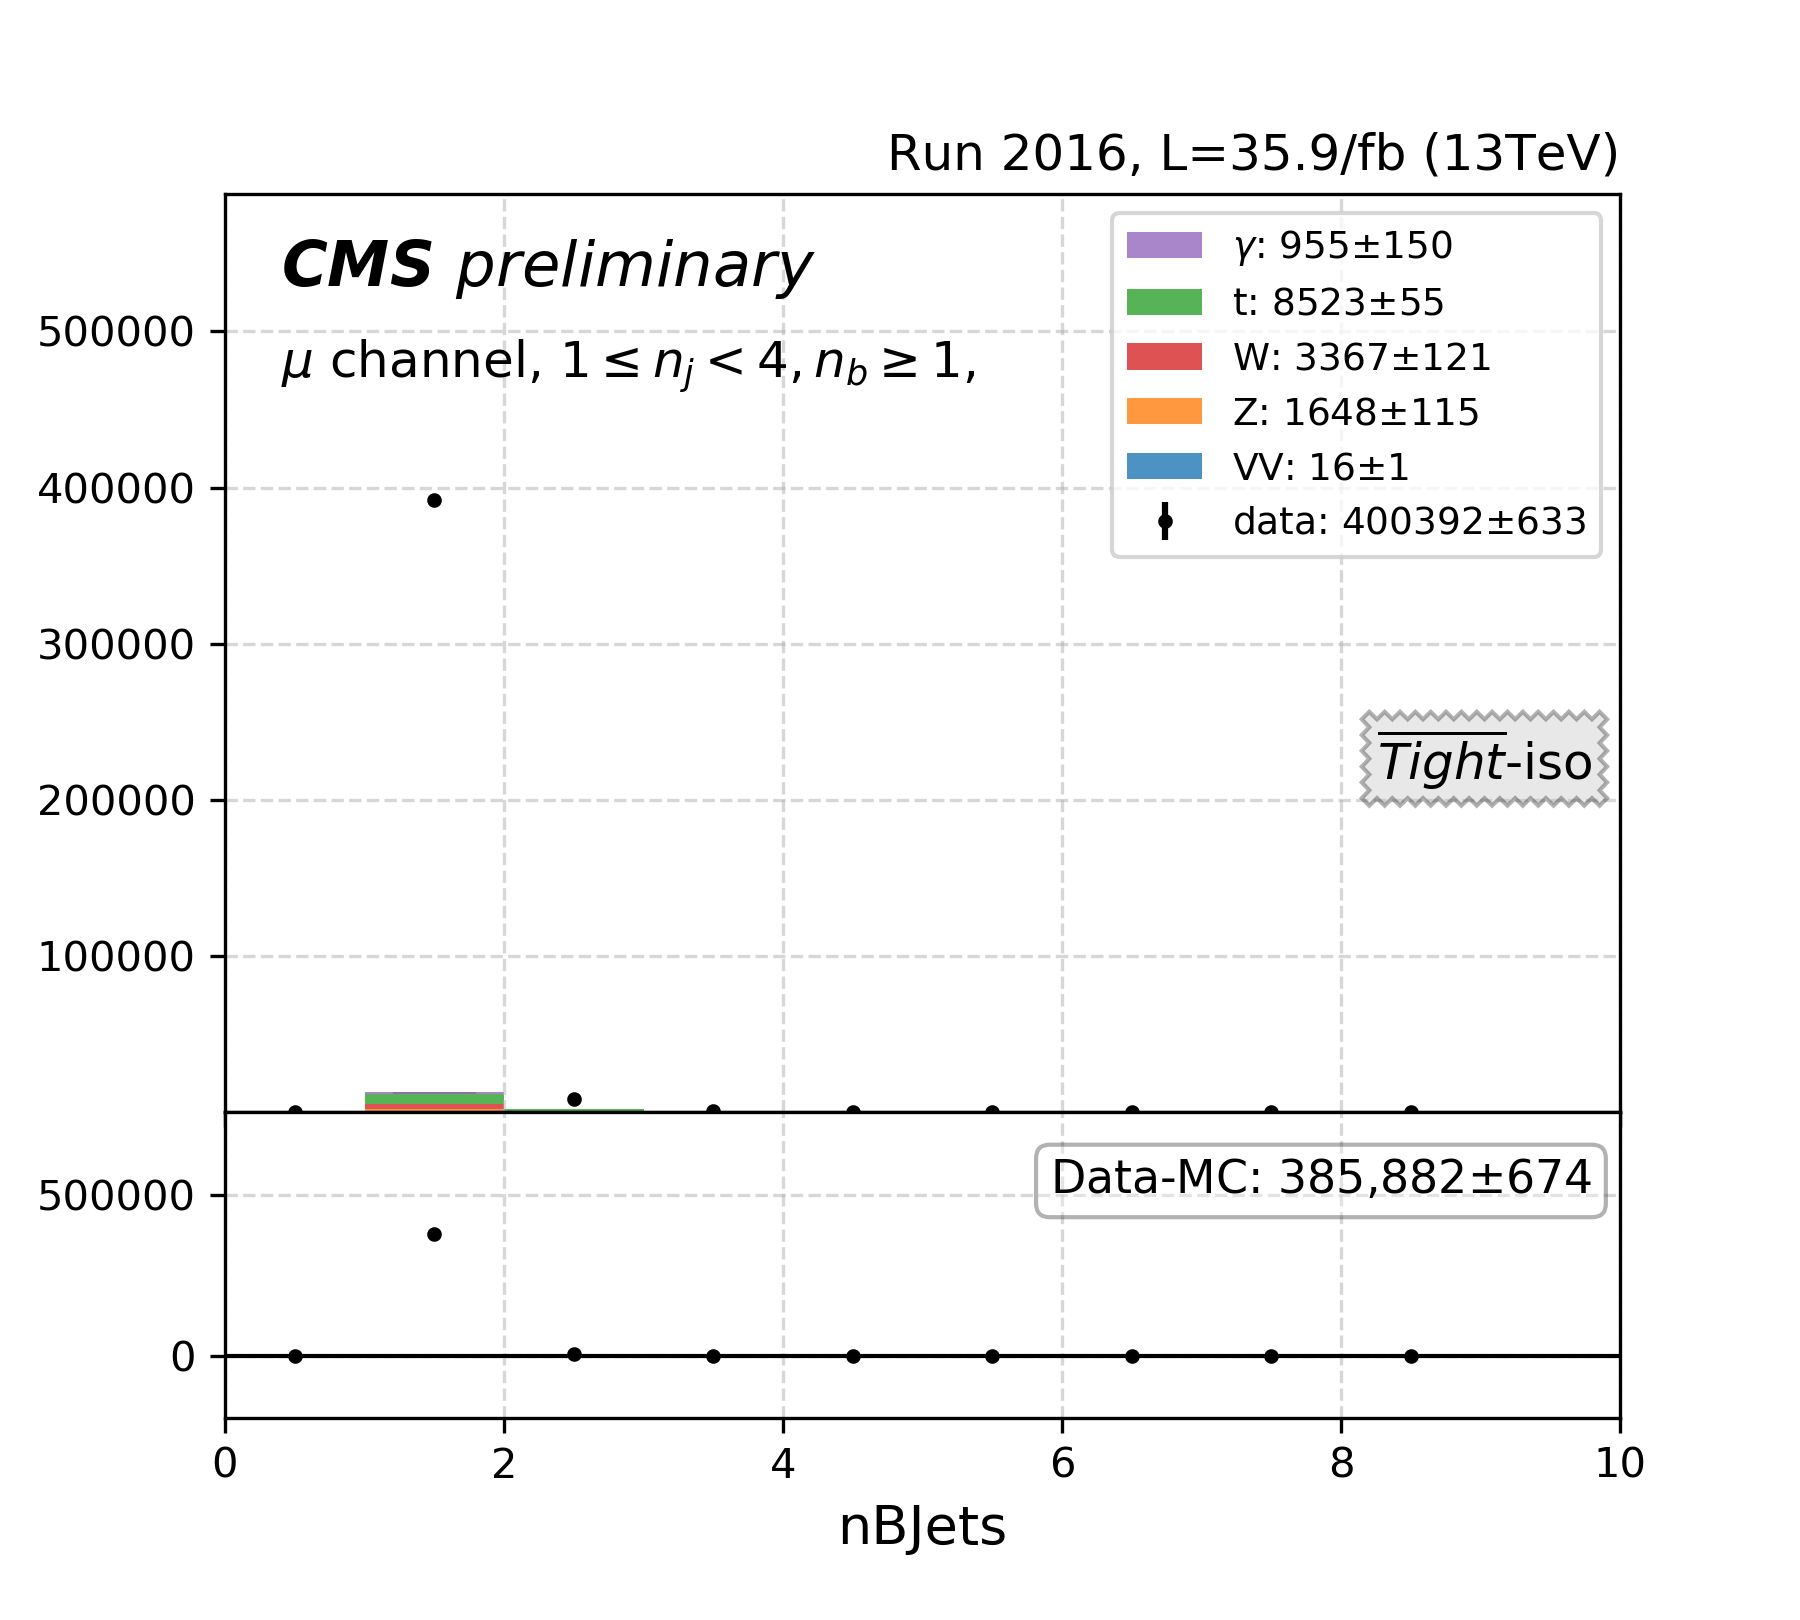
\includegraphics[width=0.24\textwidth]{appendices/qcdSF/figures/123j1b/mu_nBJets_False.png}
    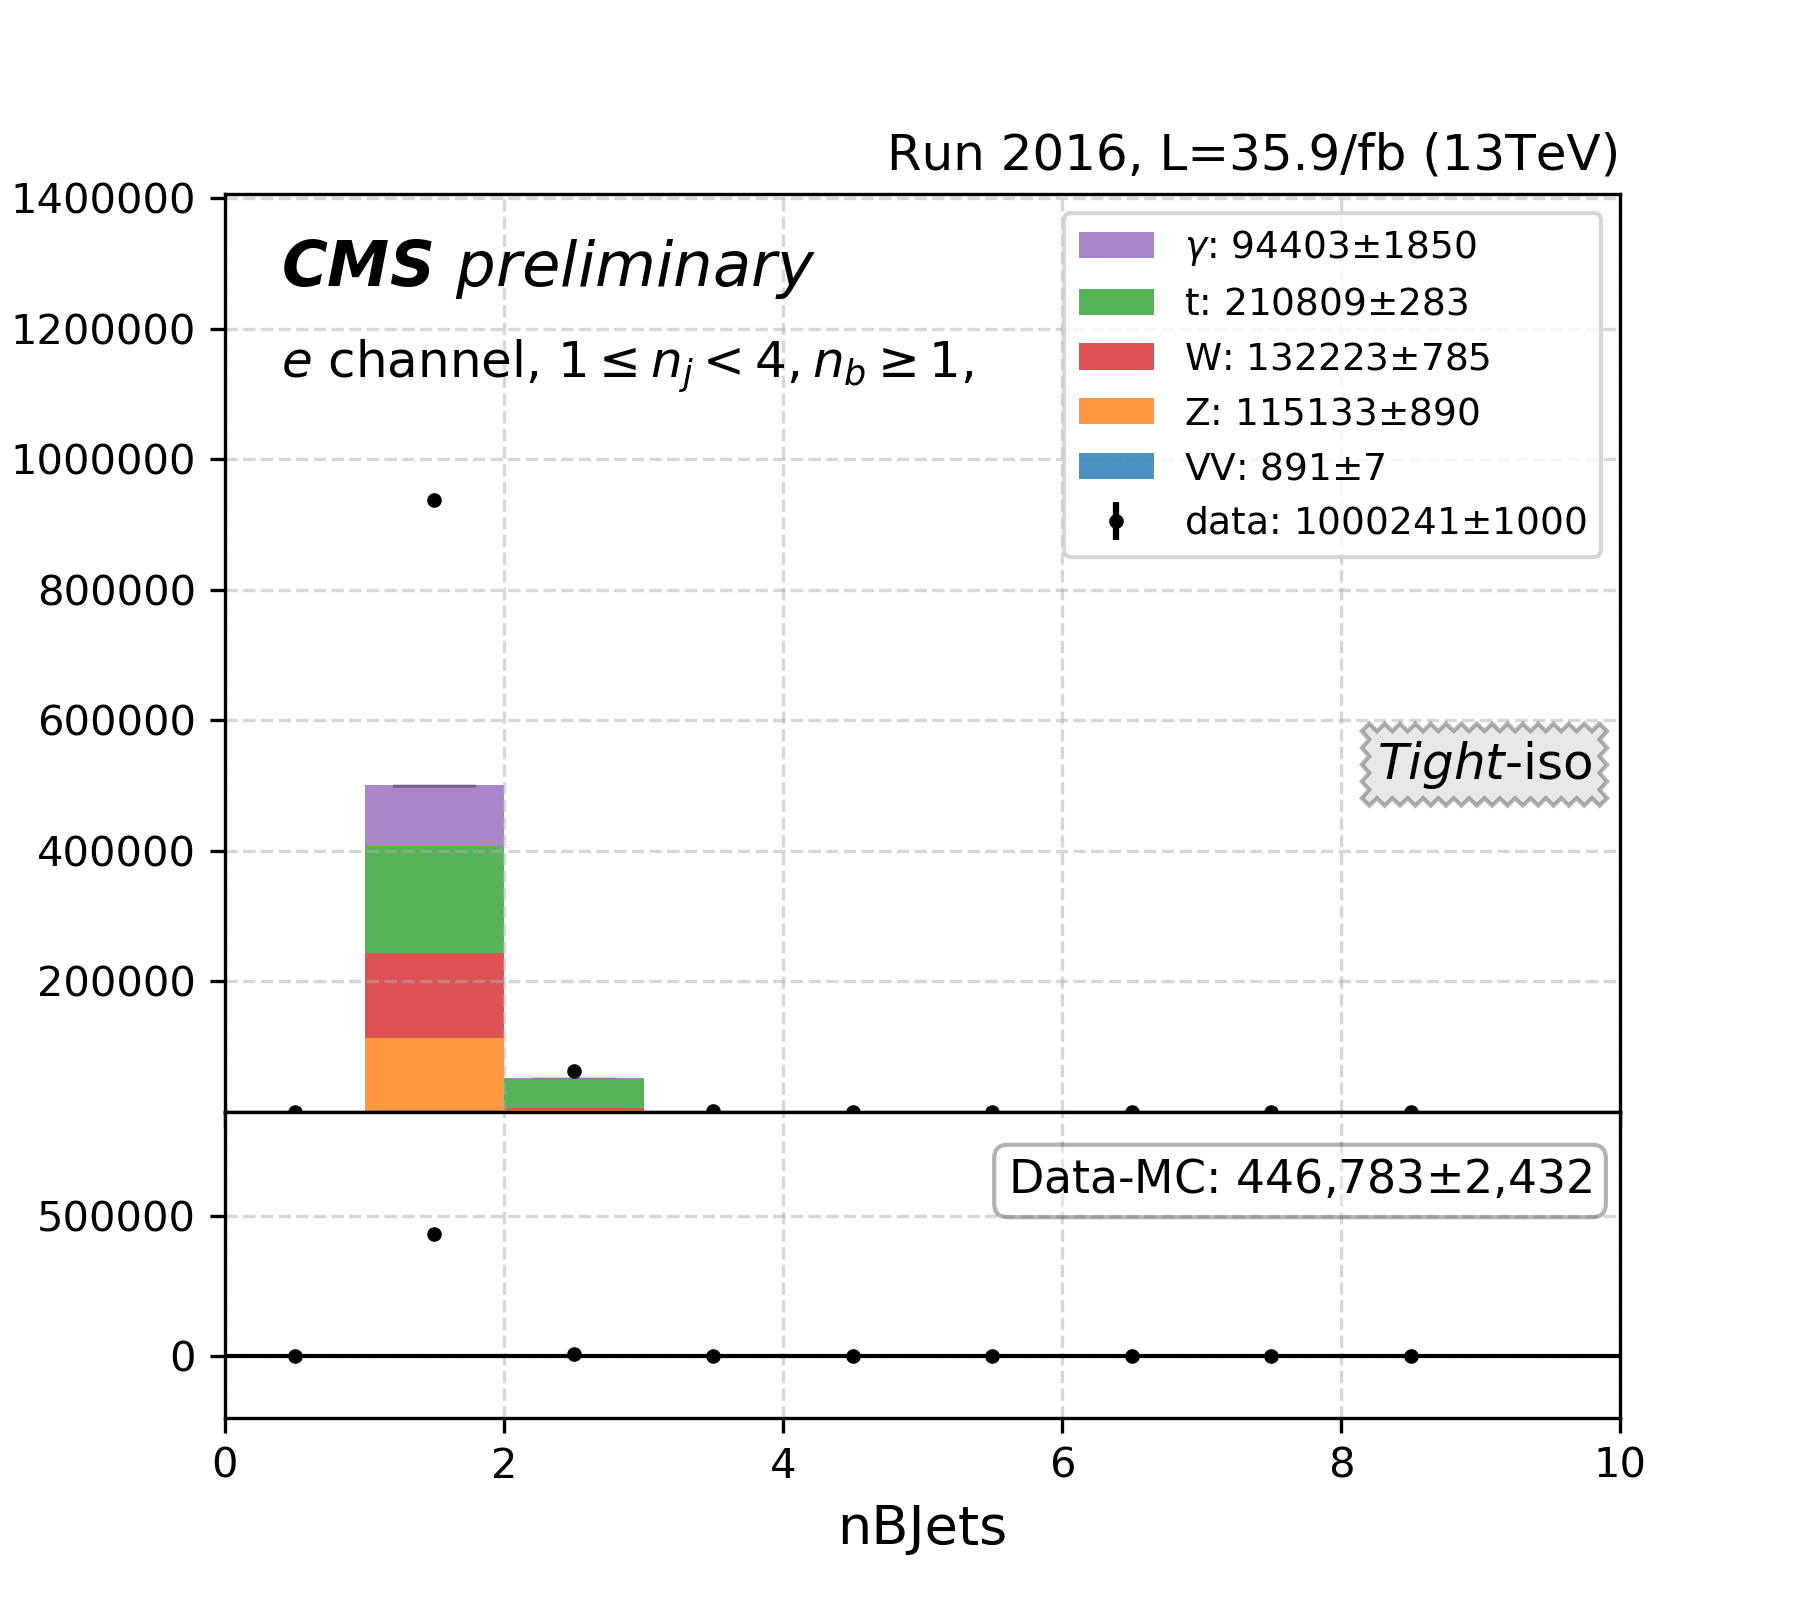
\includegraphics[width=0.24\textwidth]{appendices/qcdSF/figures/123j1b/e_nBJets_True.png}
    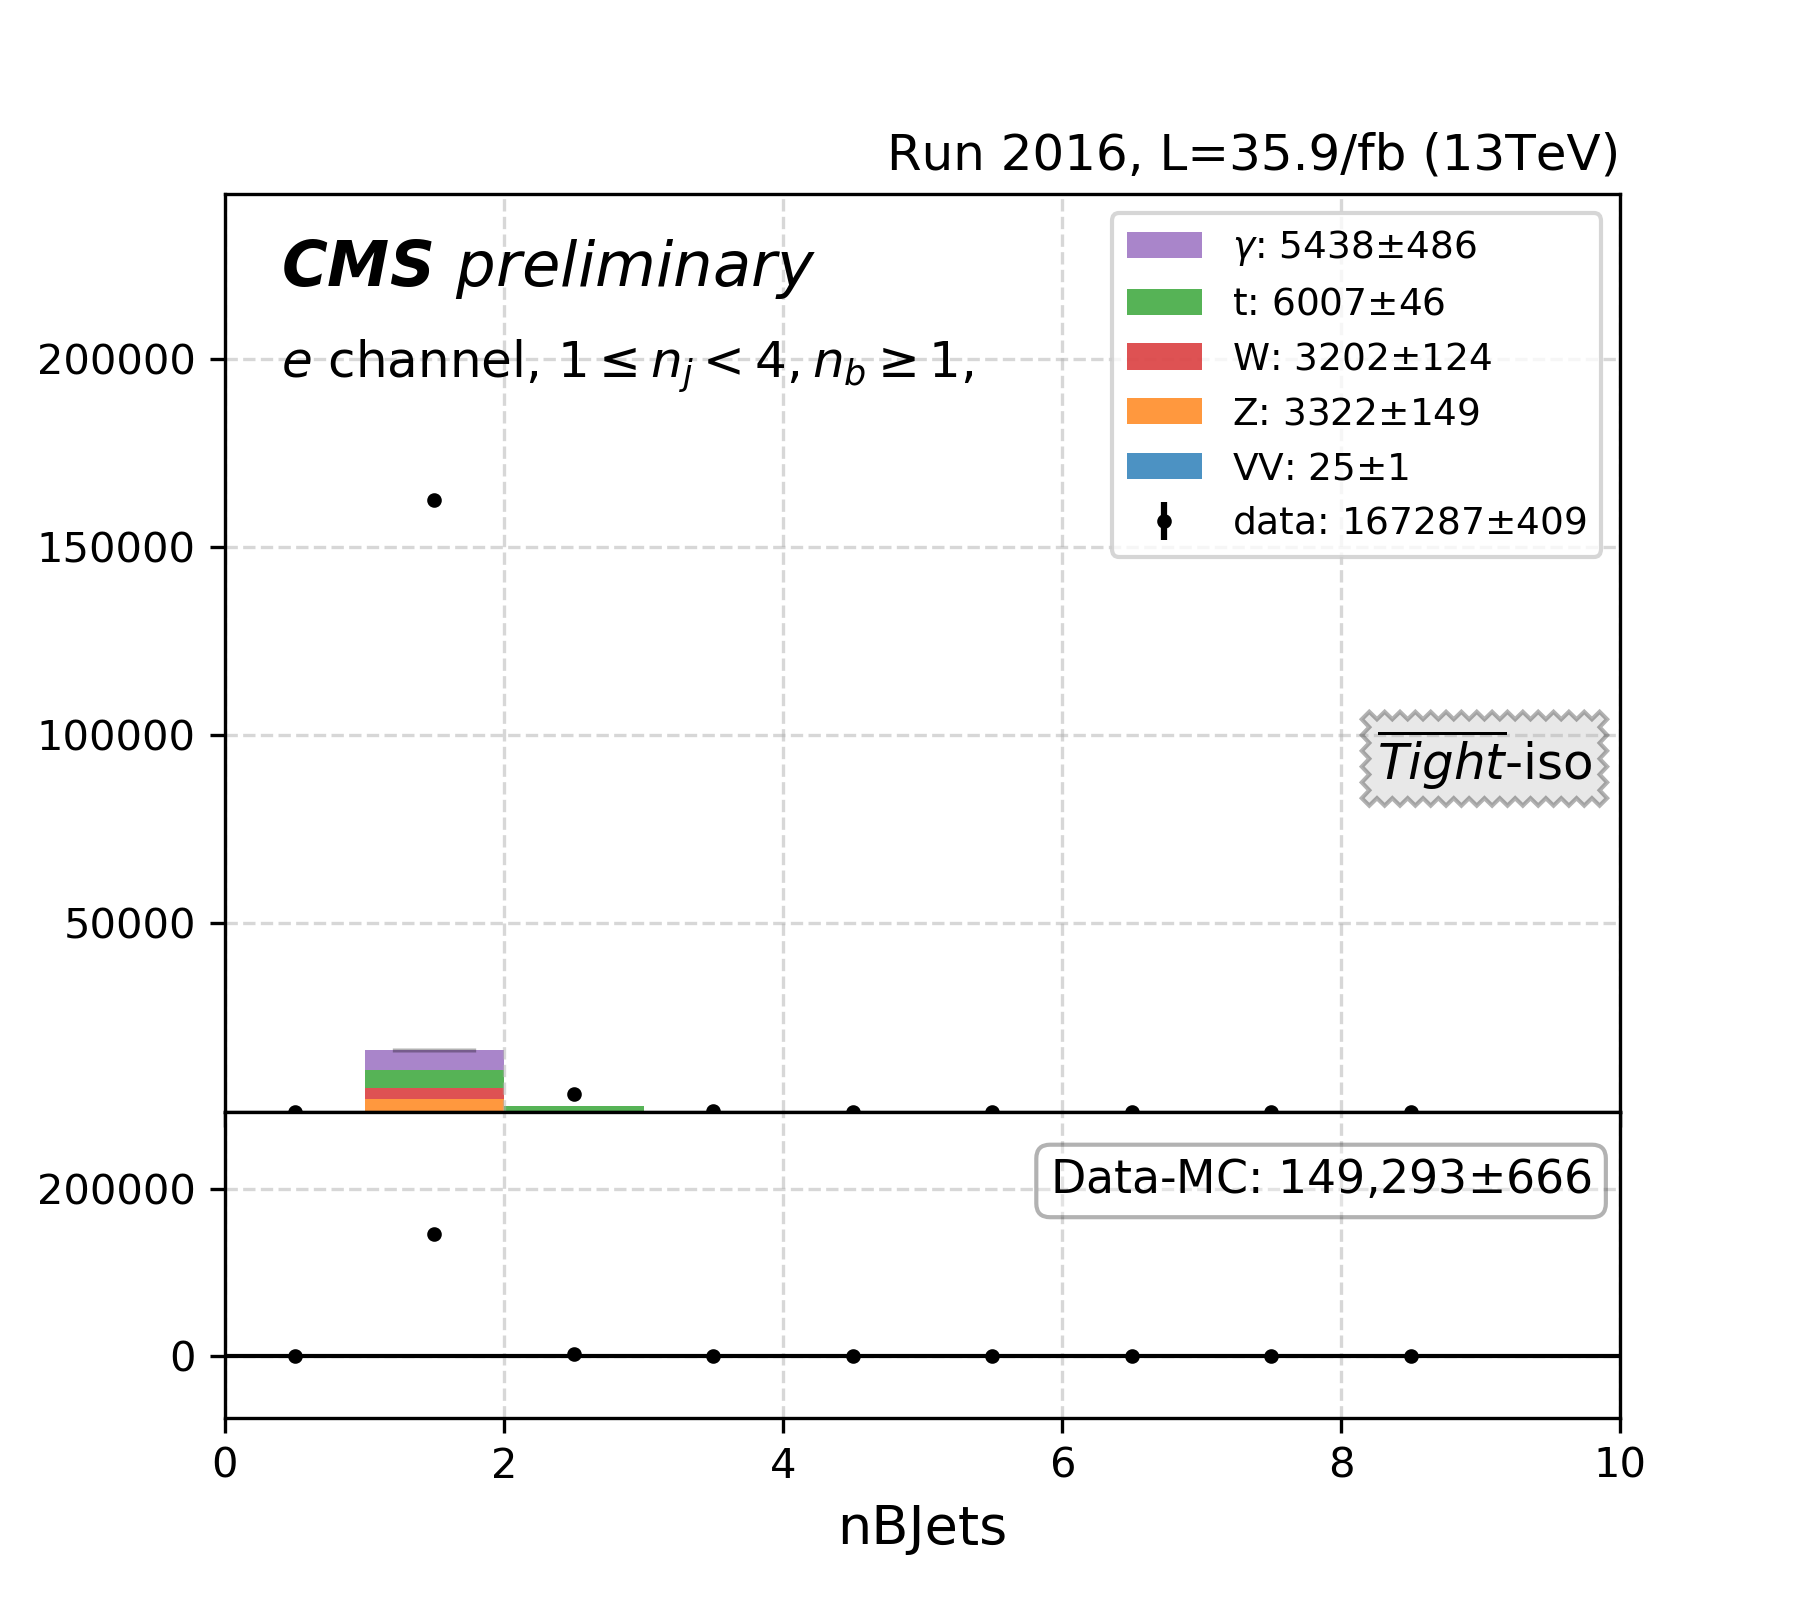
\includegraphics[width=0.24\textwidth]{appendices/qcdSF/figures/123j1b/e_nBJets_False.png}
    

    \caption{Reweight $\tau_h$ and $j \to \tau_h$ efficiencies in the dedicated FSR, ISF, MEPS, UE ttbar samples}
    \label{fig:appendix:123j1b}
\end{figure}


\begin{figure}
    \centering
    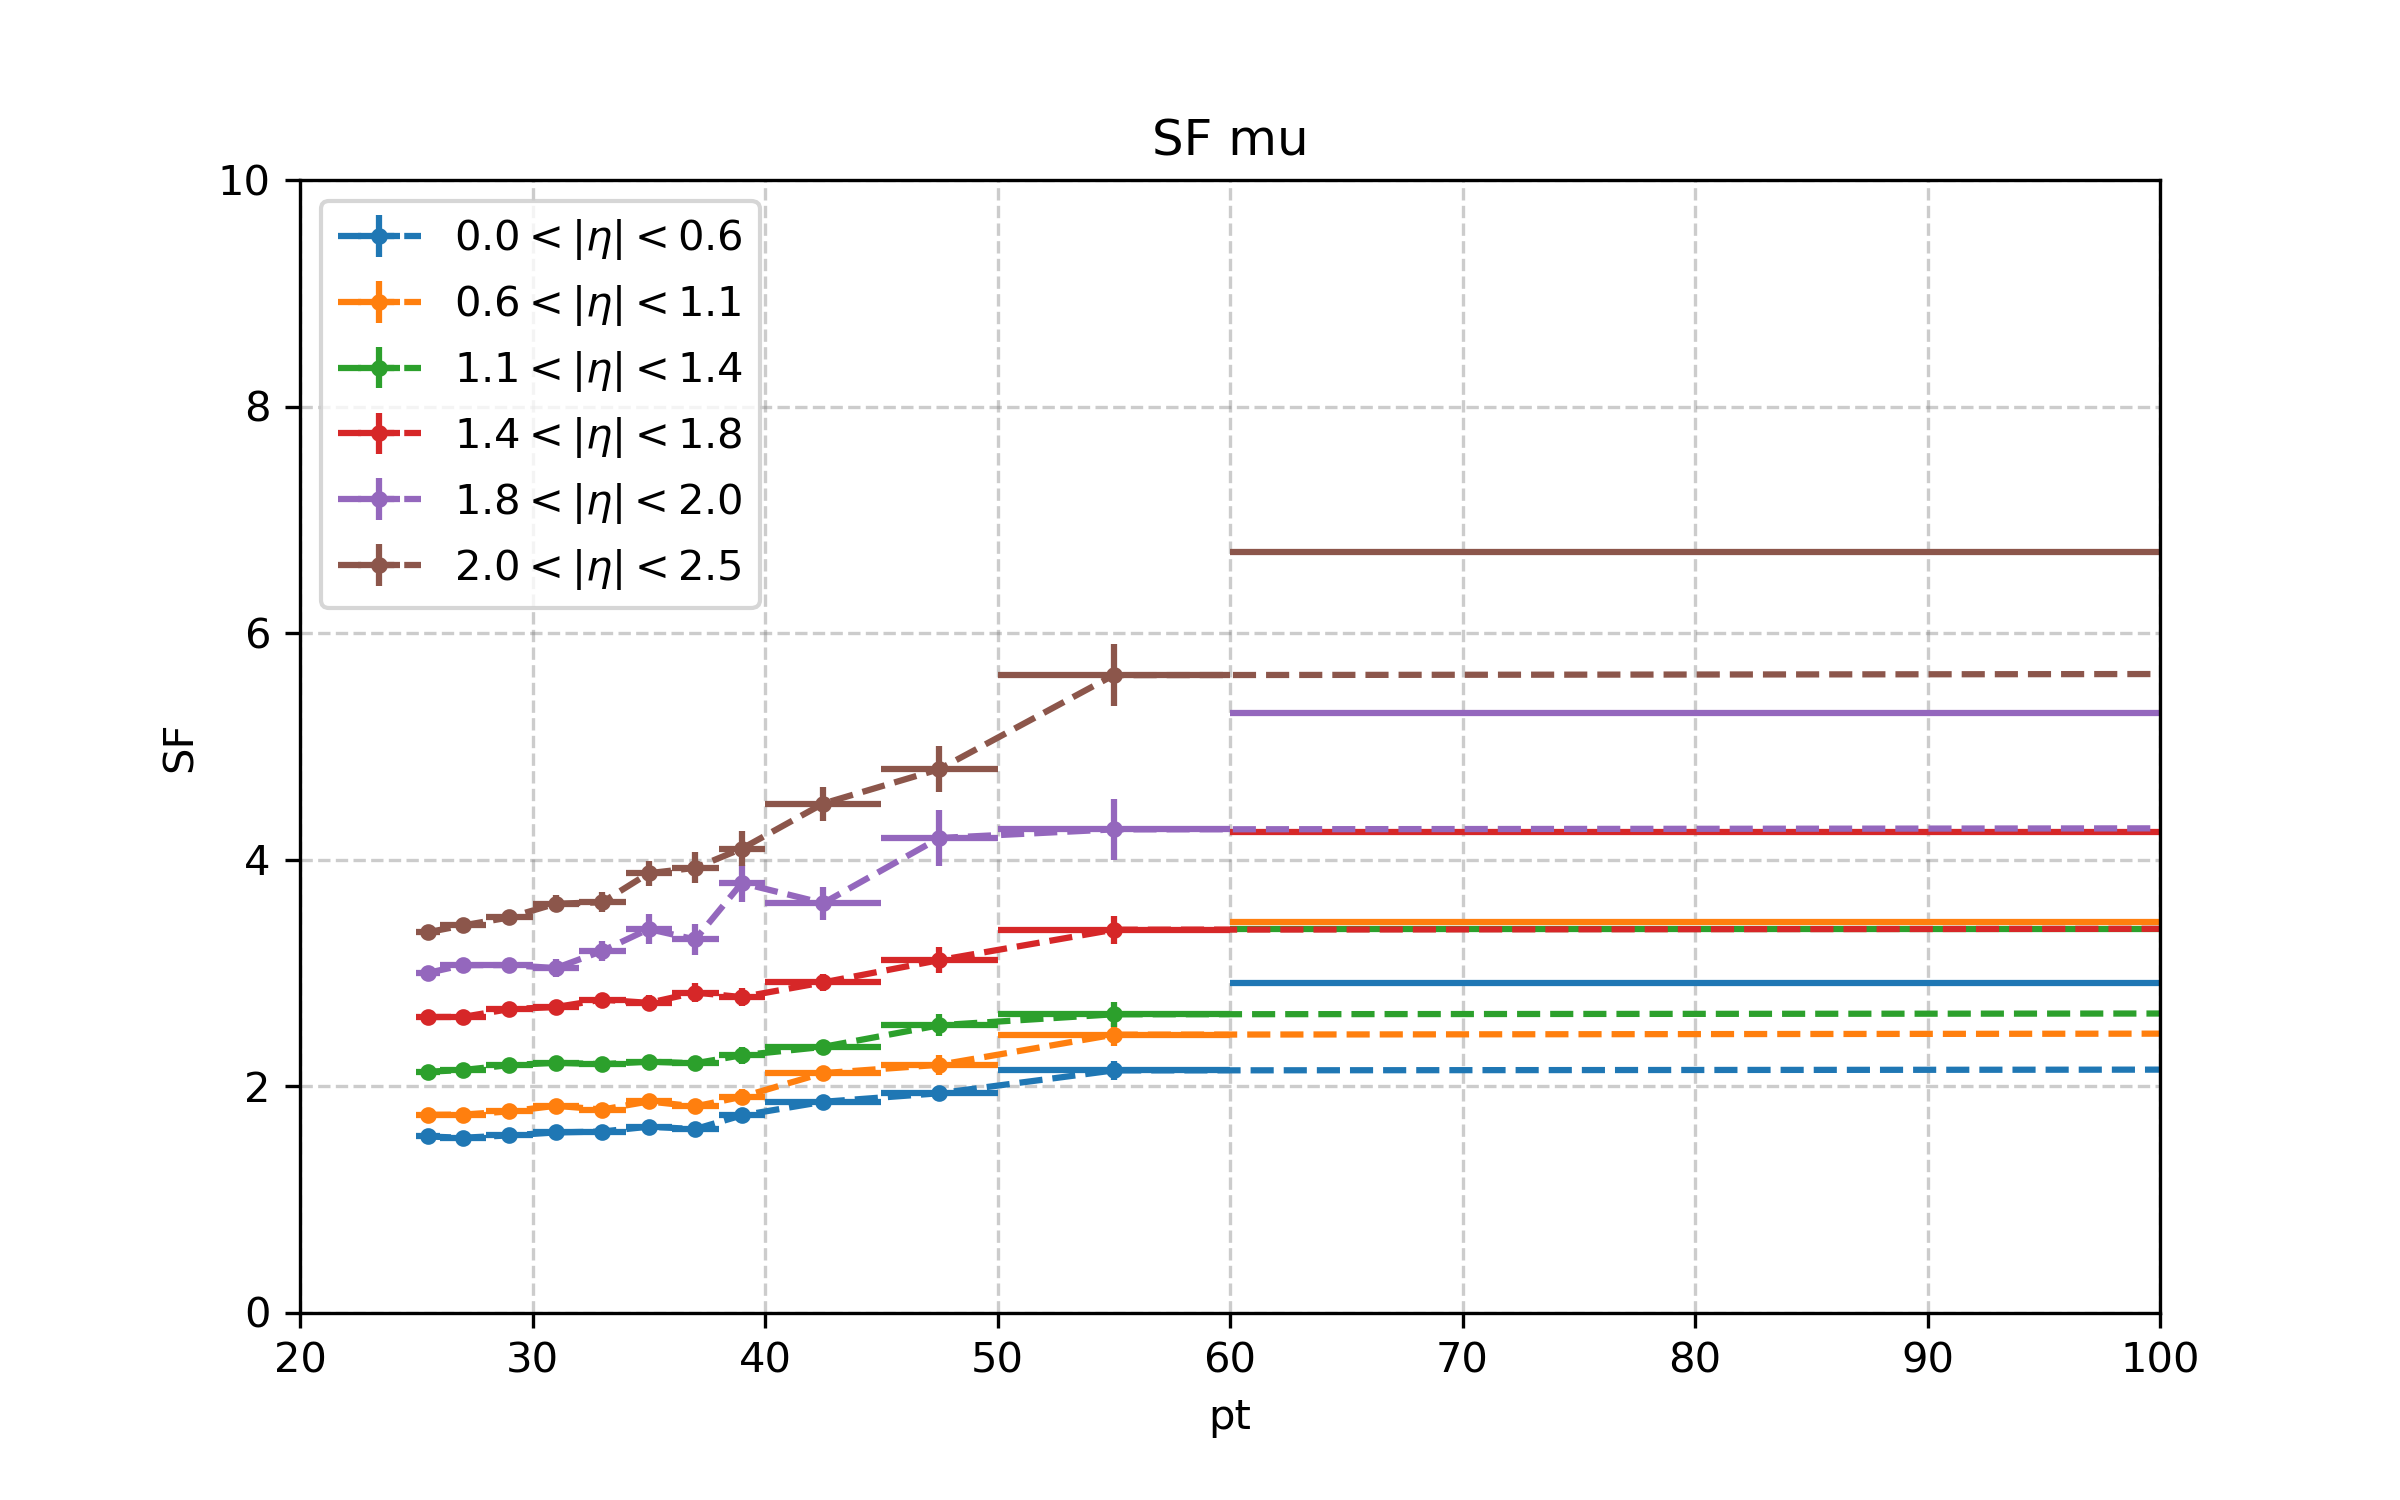
\includegraphics[width=0.49\textwidth]{appendices/qcdSF/figures/123j1b/SF_mu_1d.png}
    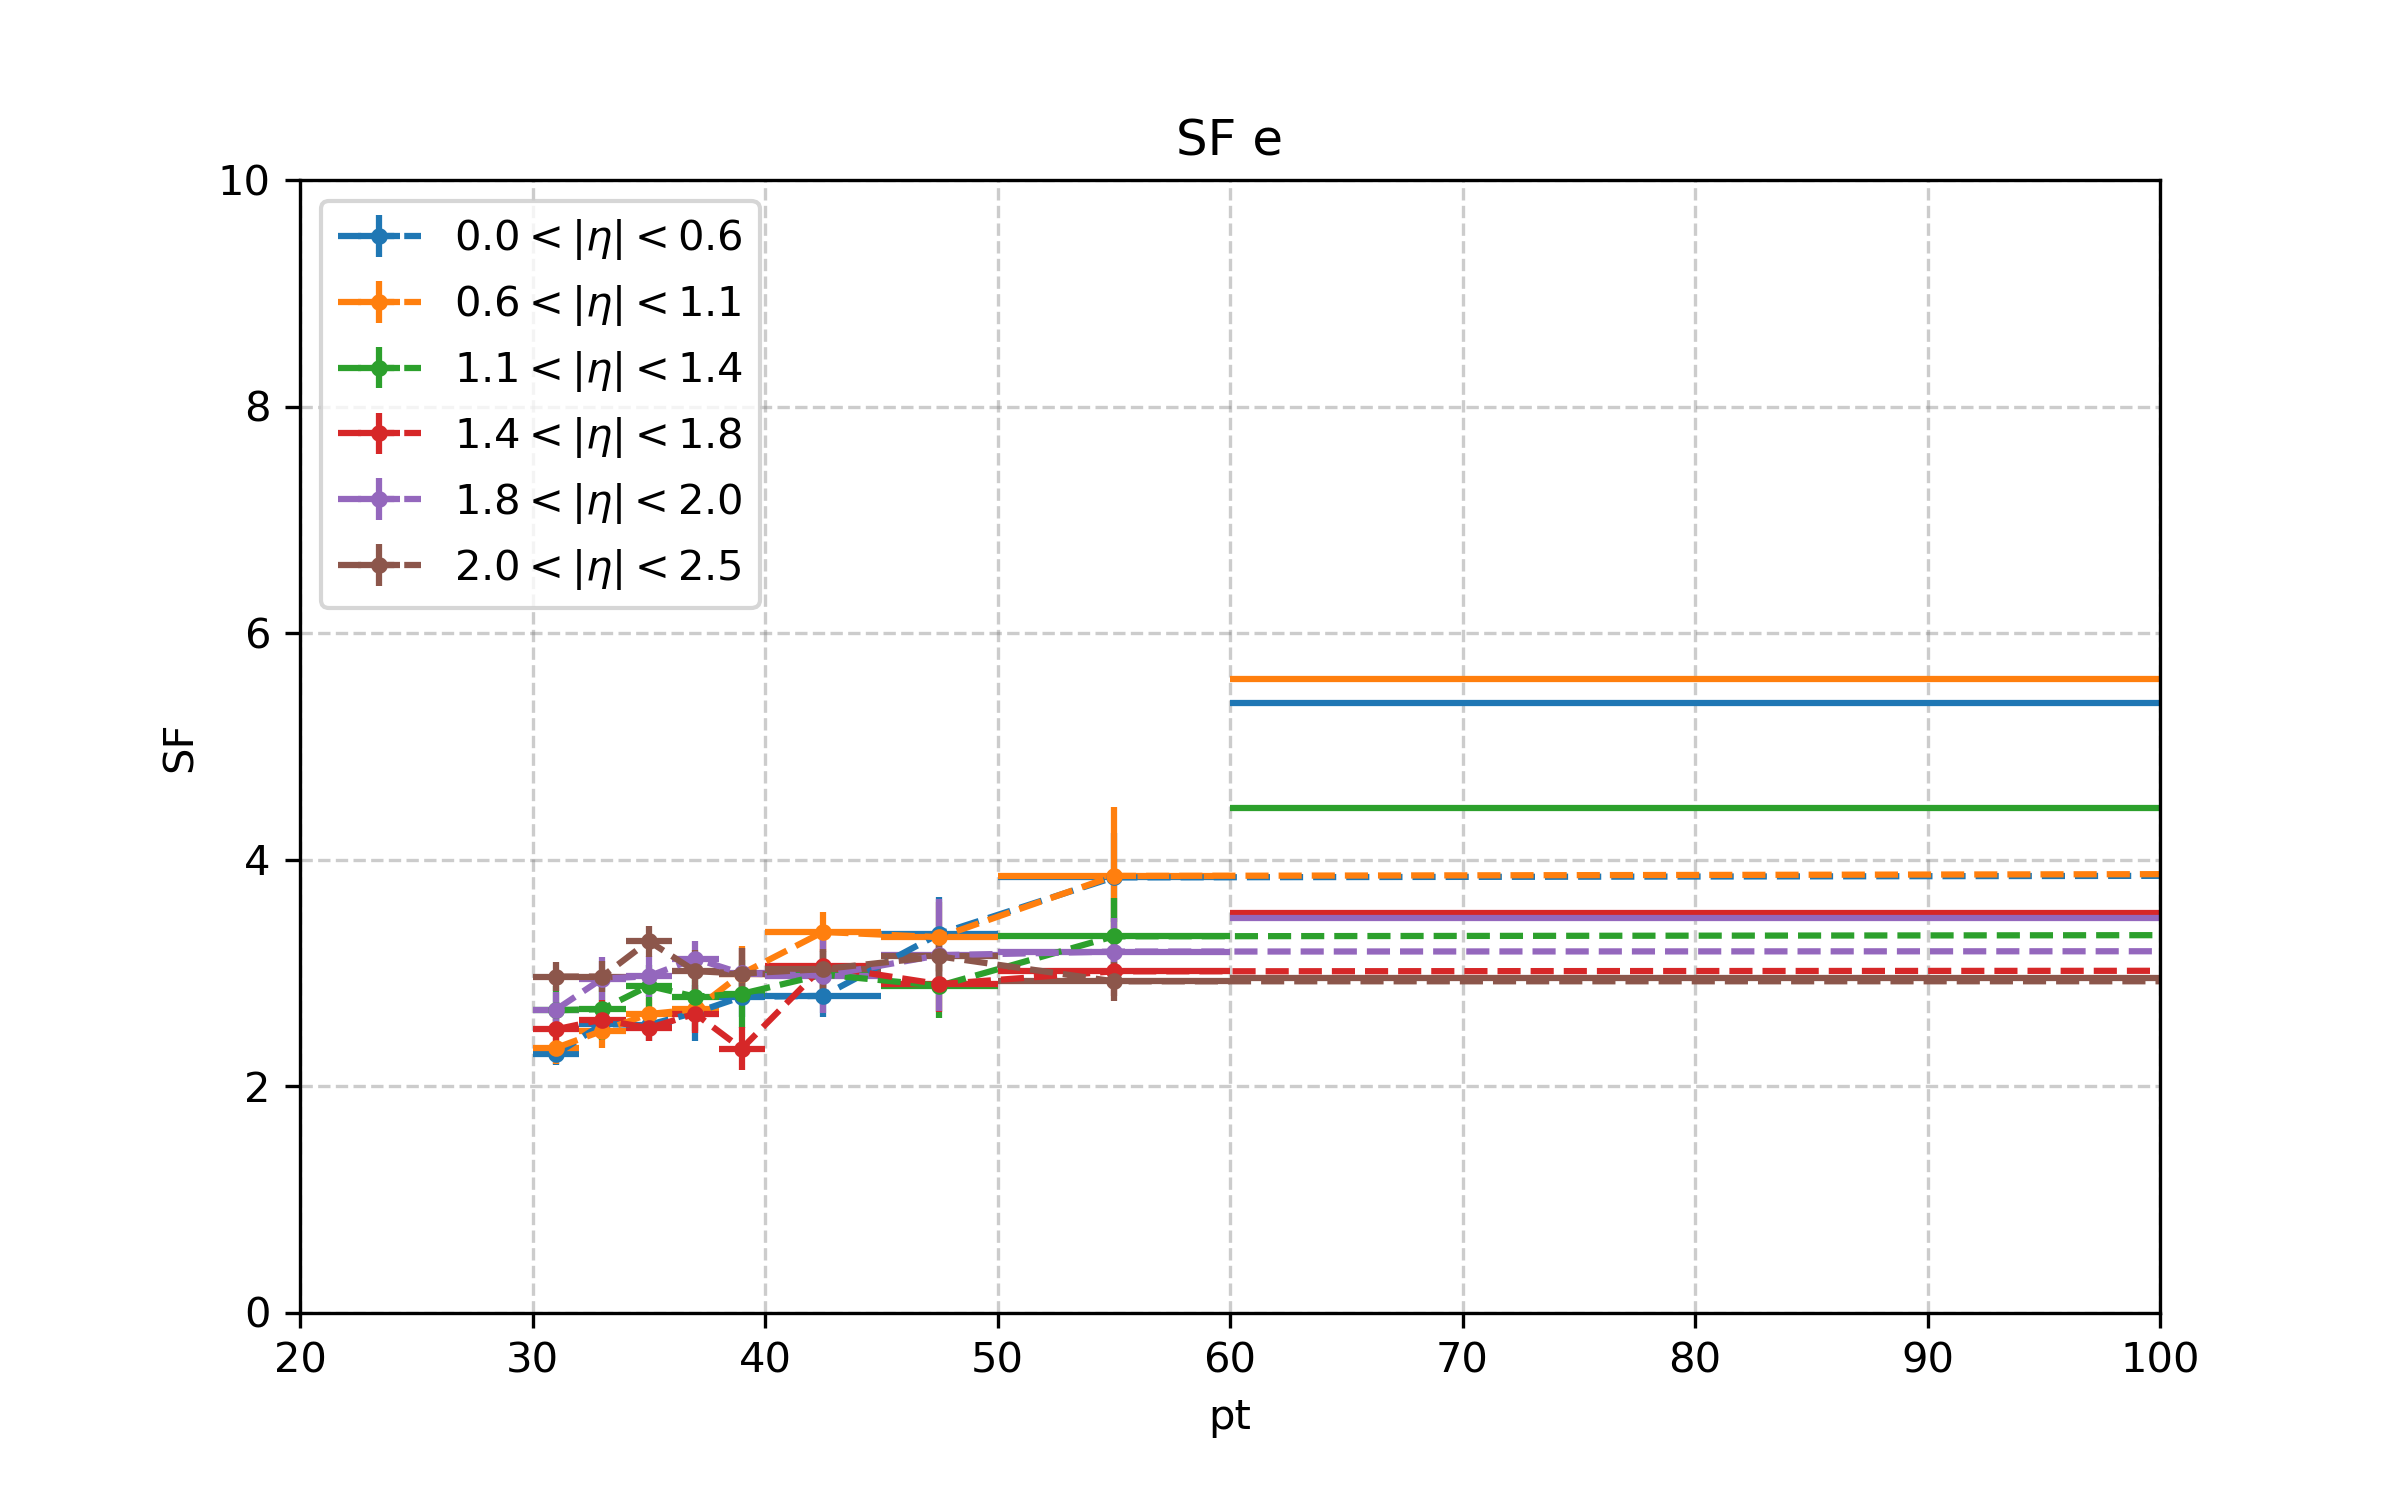
\includegraphics[width=0.49\textwidth]{appendices/qcdSF/figures/123j1b/SF_e_1d.png}
    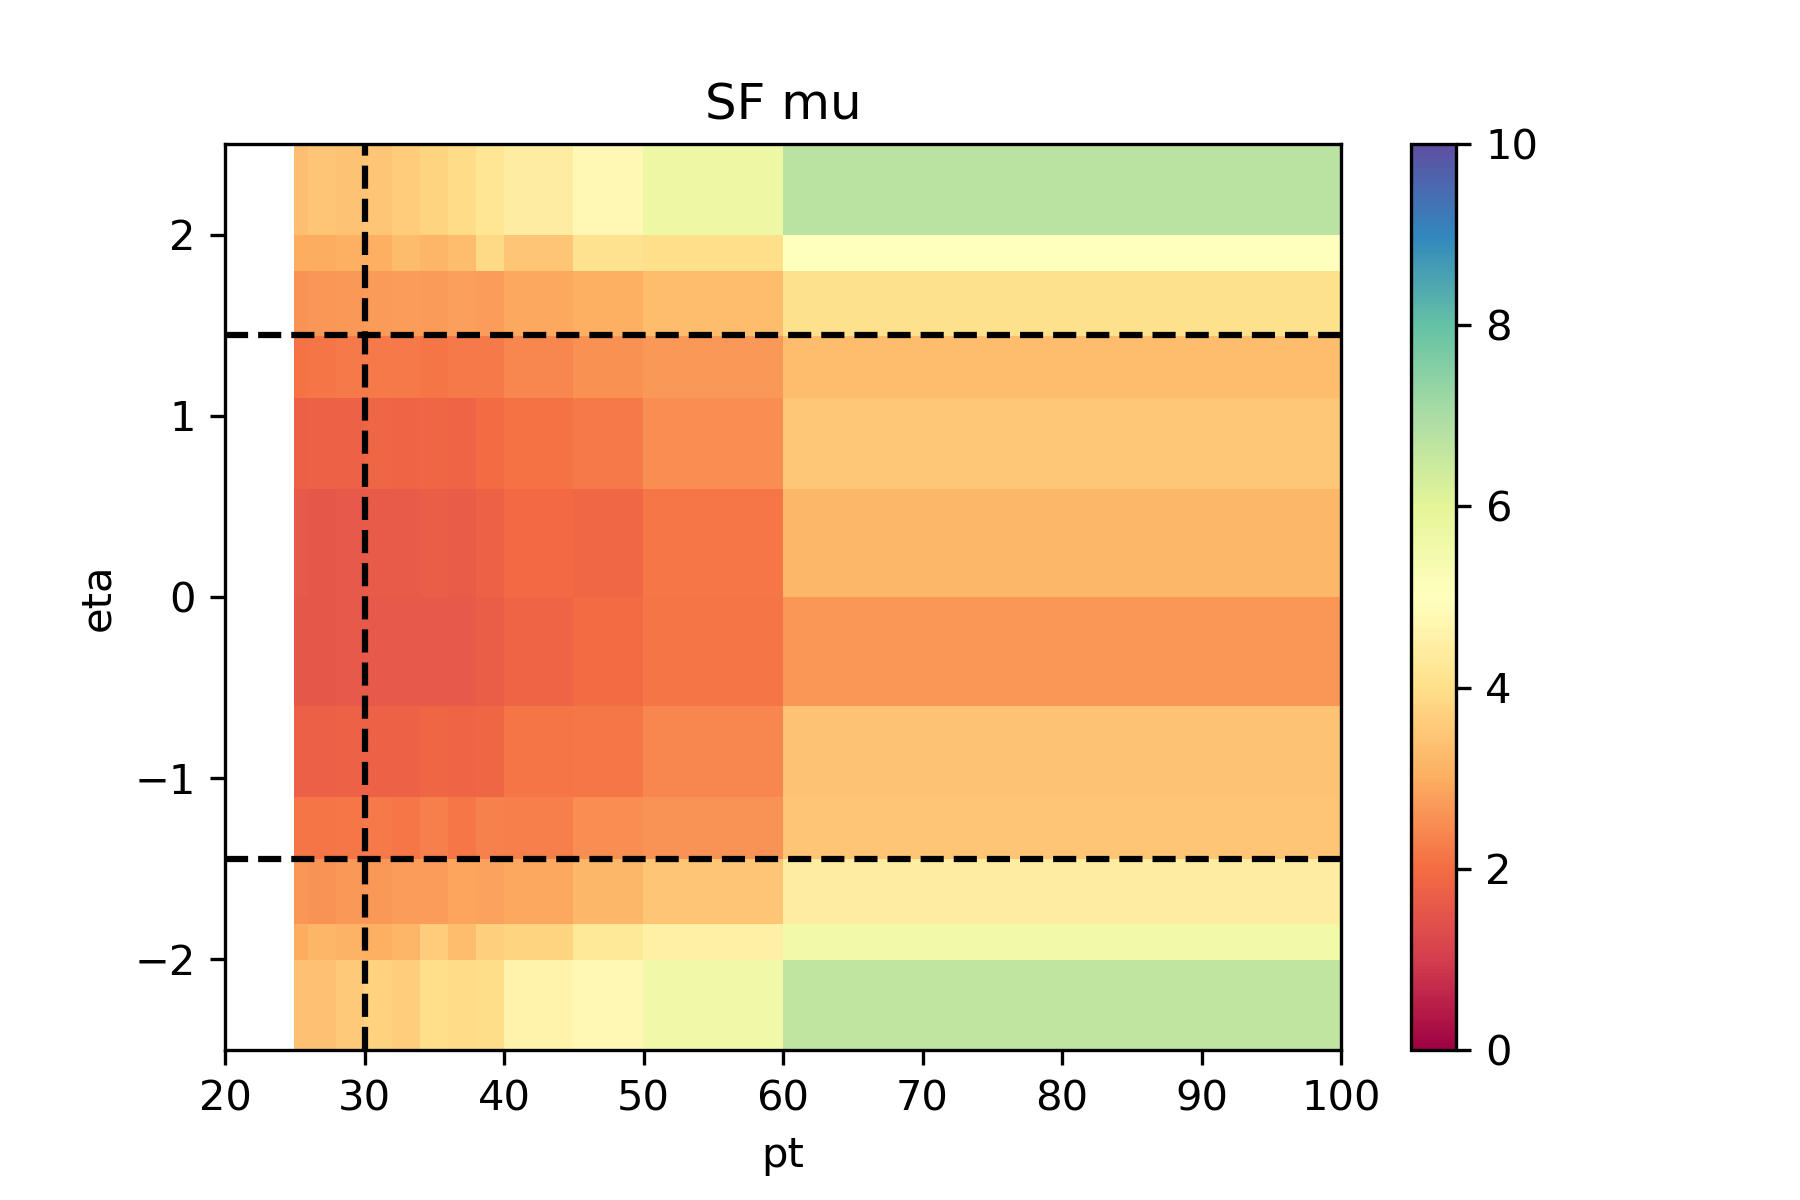
\includegraphics[width=0.49\textwidth]{appendices/qcdSF/figures/123j1b/SF_mu_2d.png}
    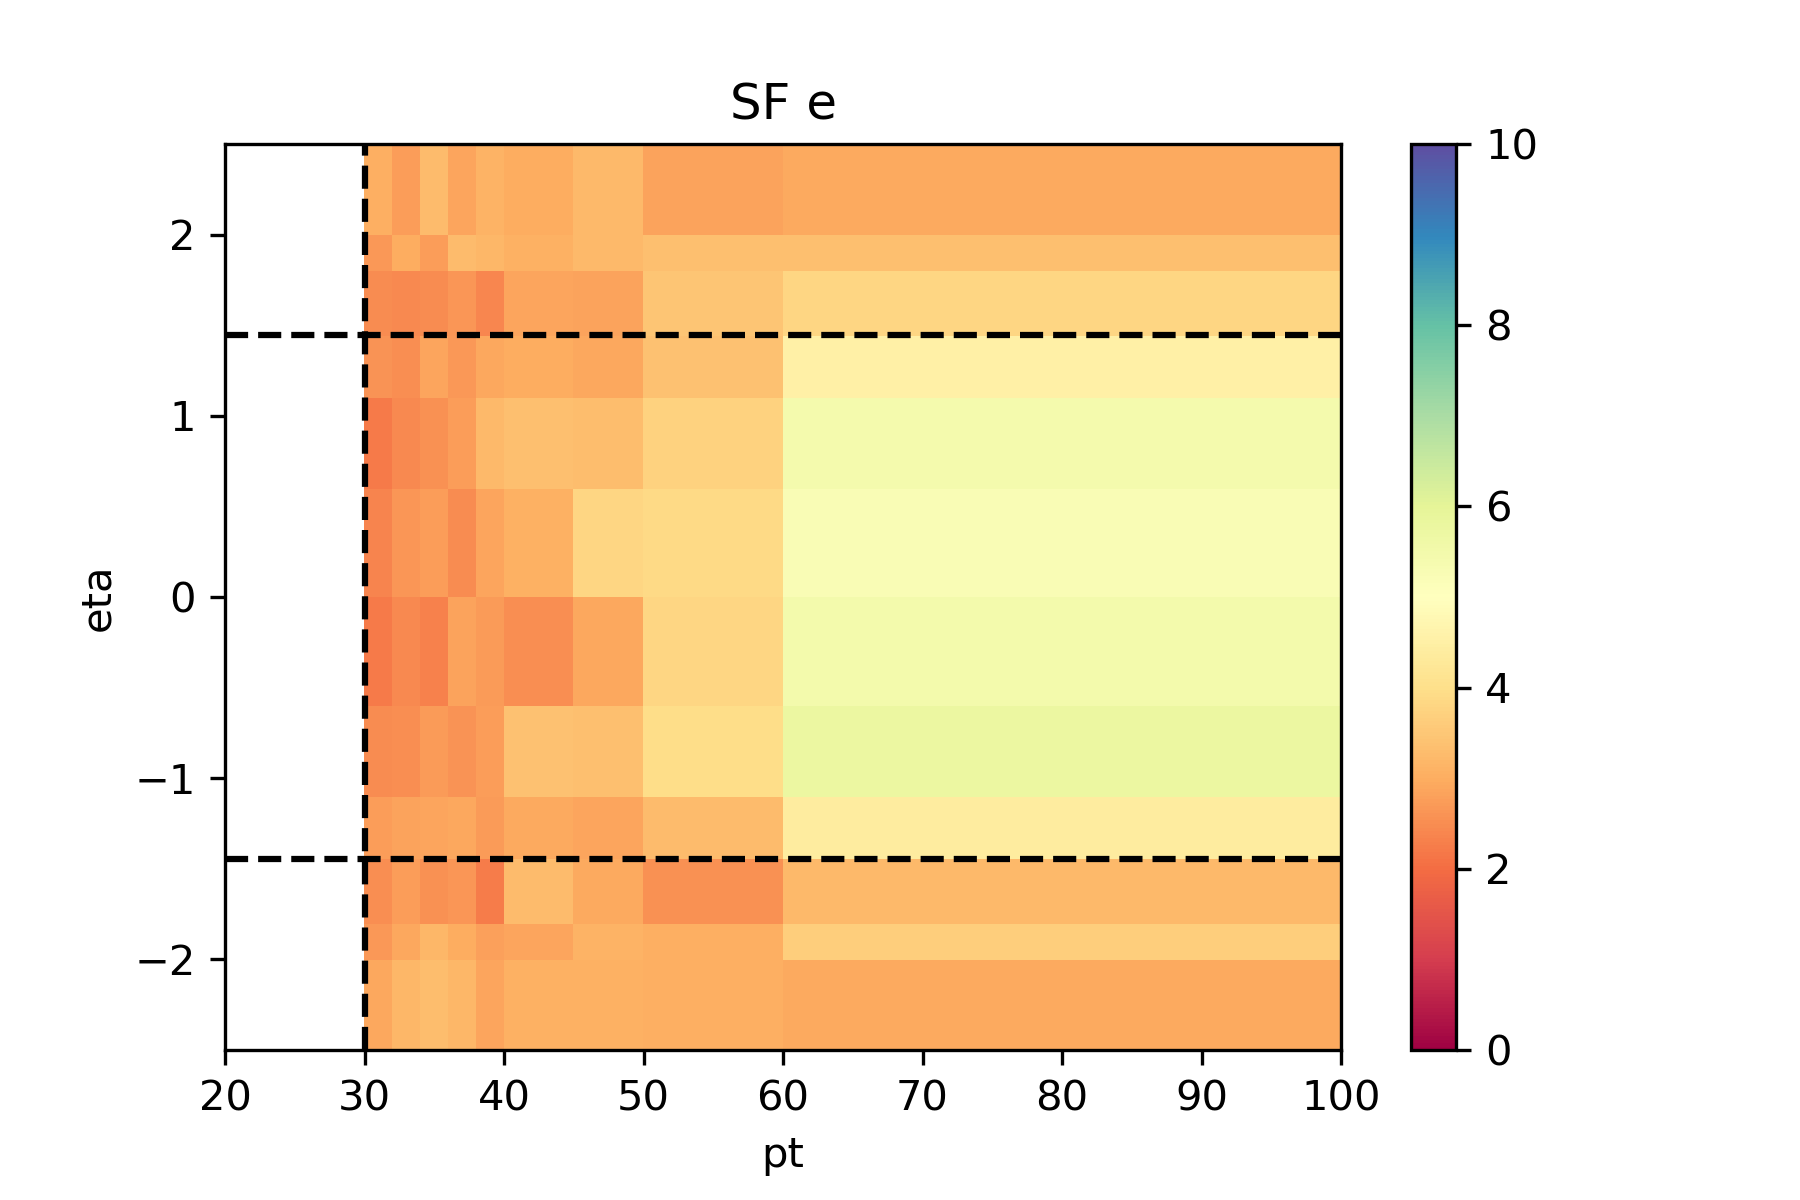
\includegraphics[width=0.49\textwidth]{appendices/qcdSF/figures/123j1b/SF_e_2d.png}

    \caption{Reweight $\tau_h$ and $j \to \tau_h$ efficiencies in the dedicated FSR, ISF, MEPS, UE ttbar samples}
    \label{fig:appendix:123j1b}
\end{figure}



\begin{figure}
    \centering
    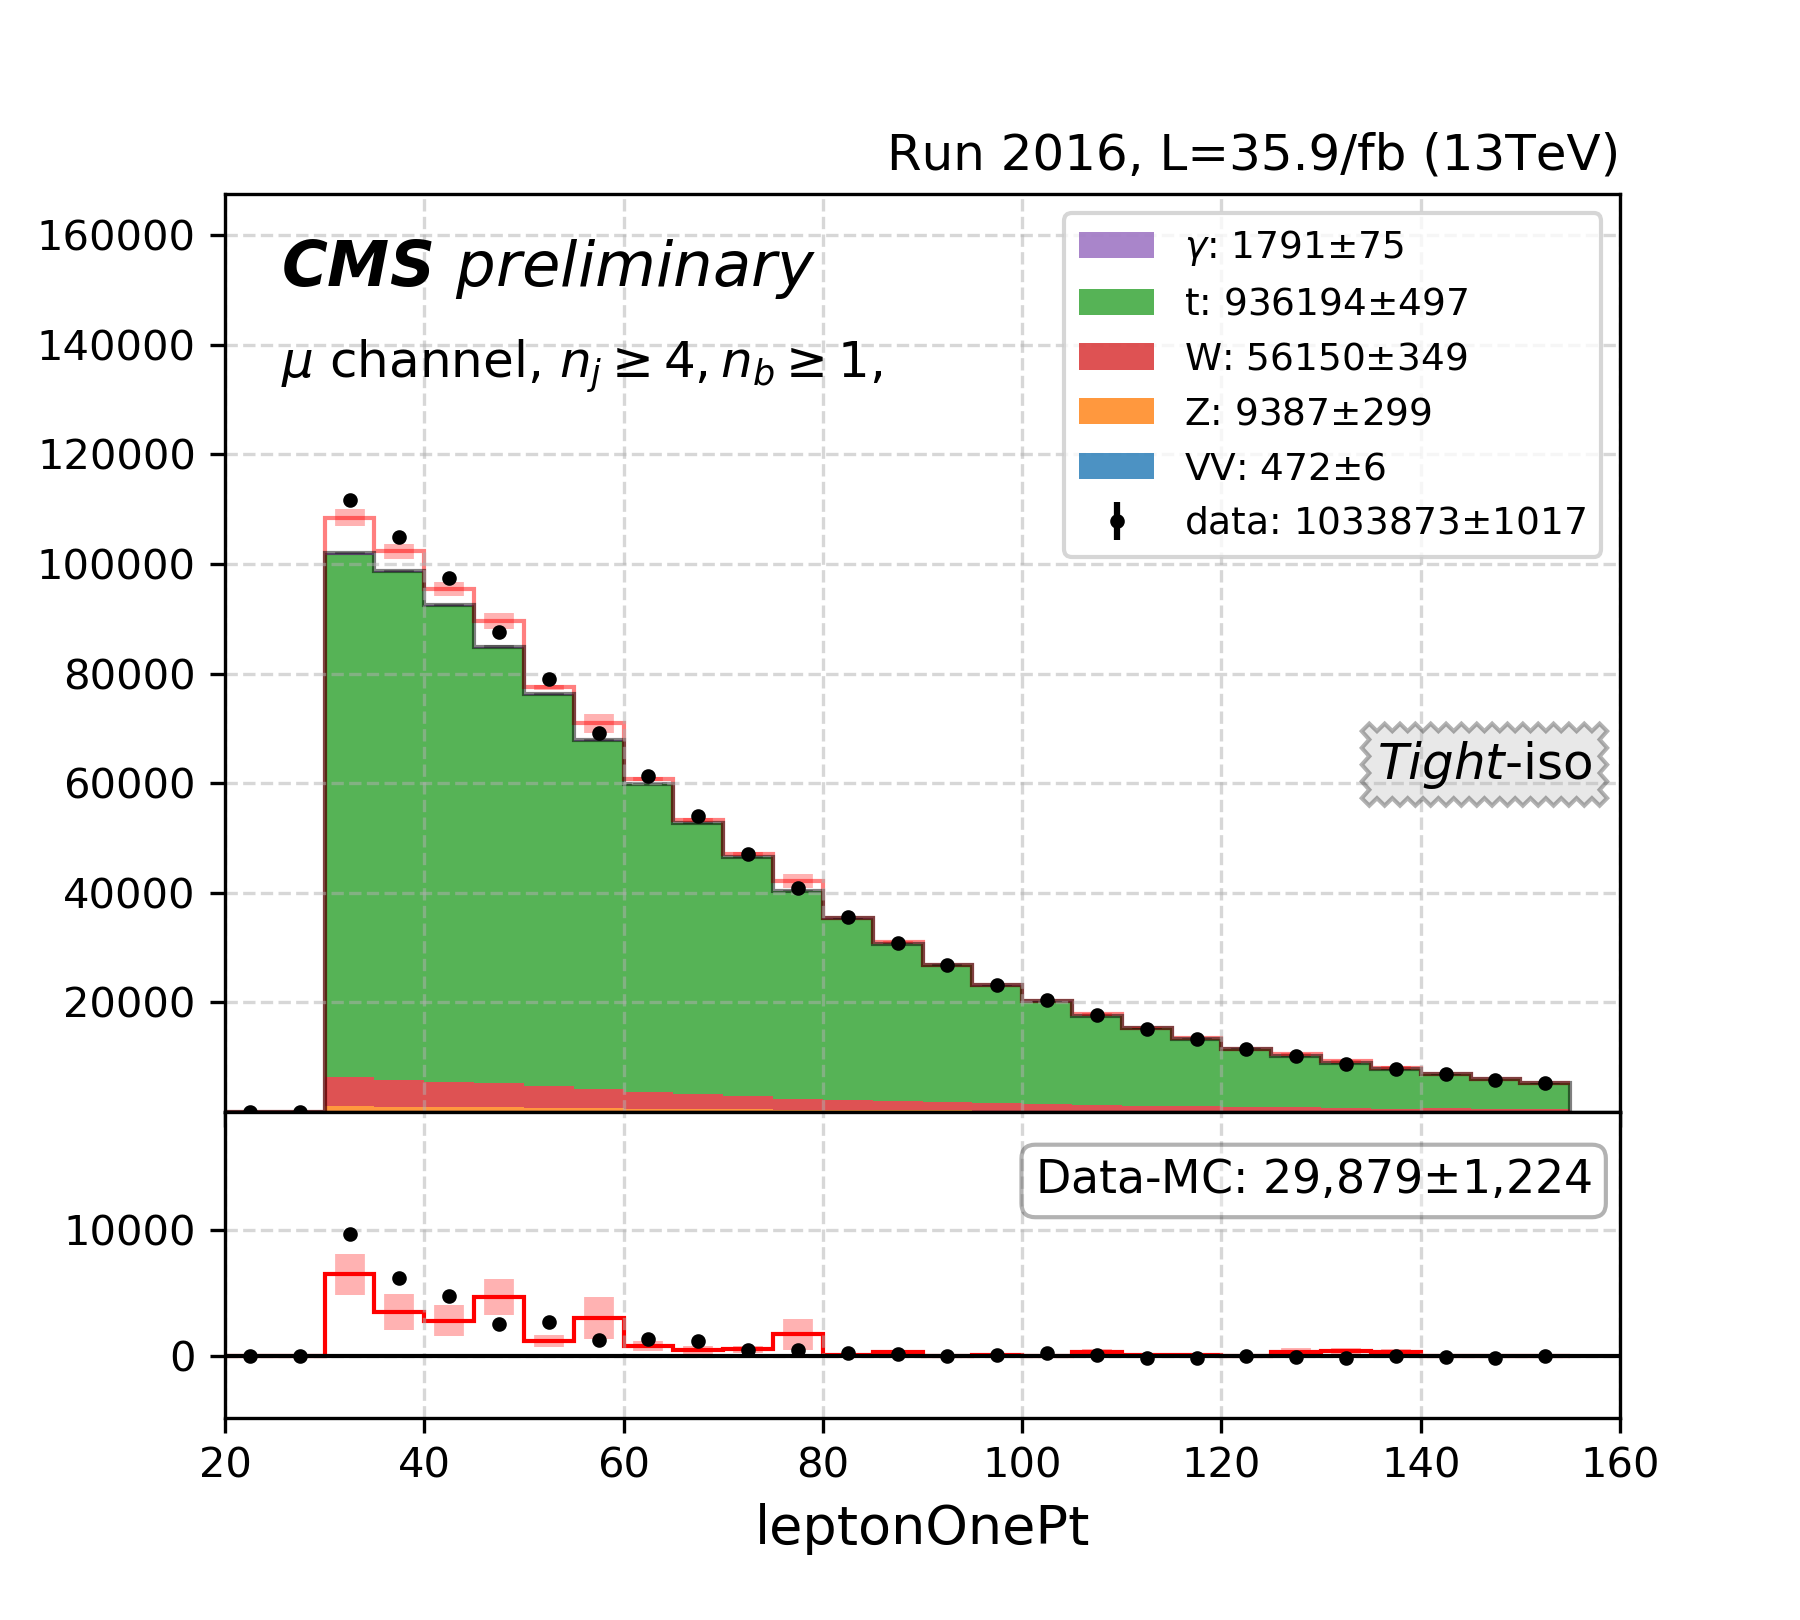
\includegraphics[width=0.24\textwidth]{appendices/qcdSF/figures/4j1b/mu_leptonOnePt_True_mcqcd.png}
    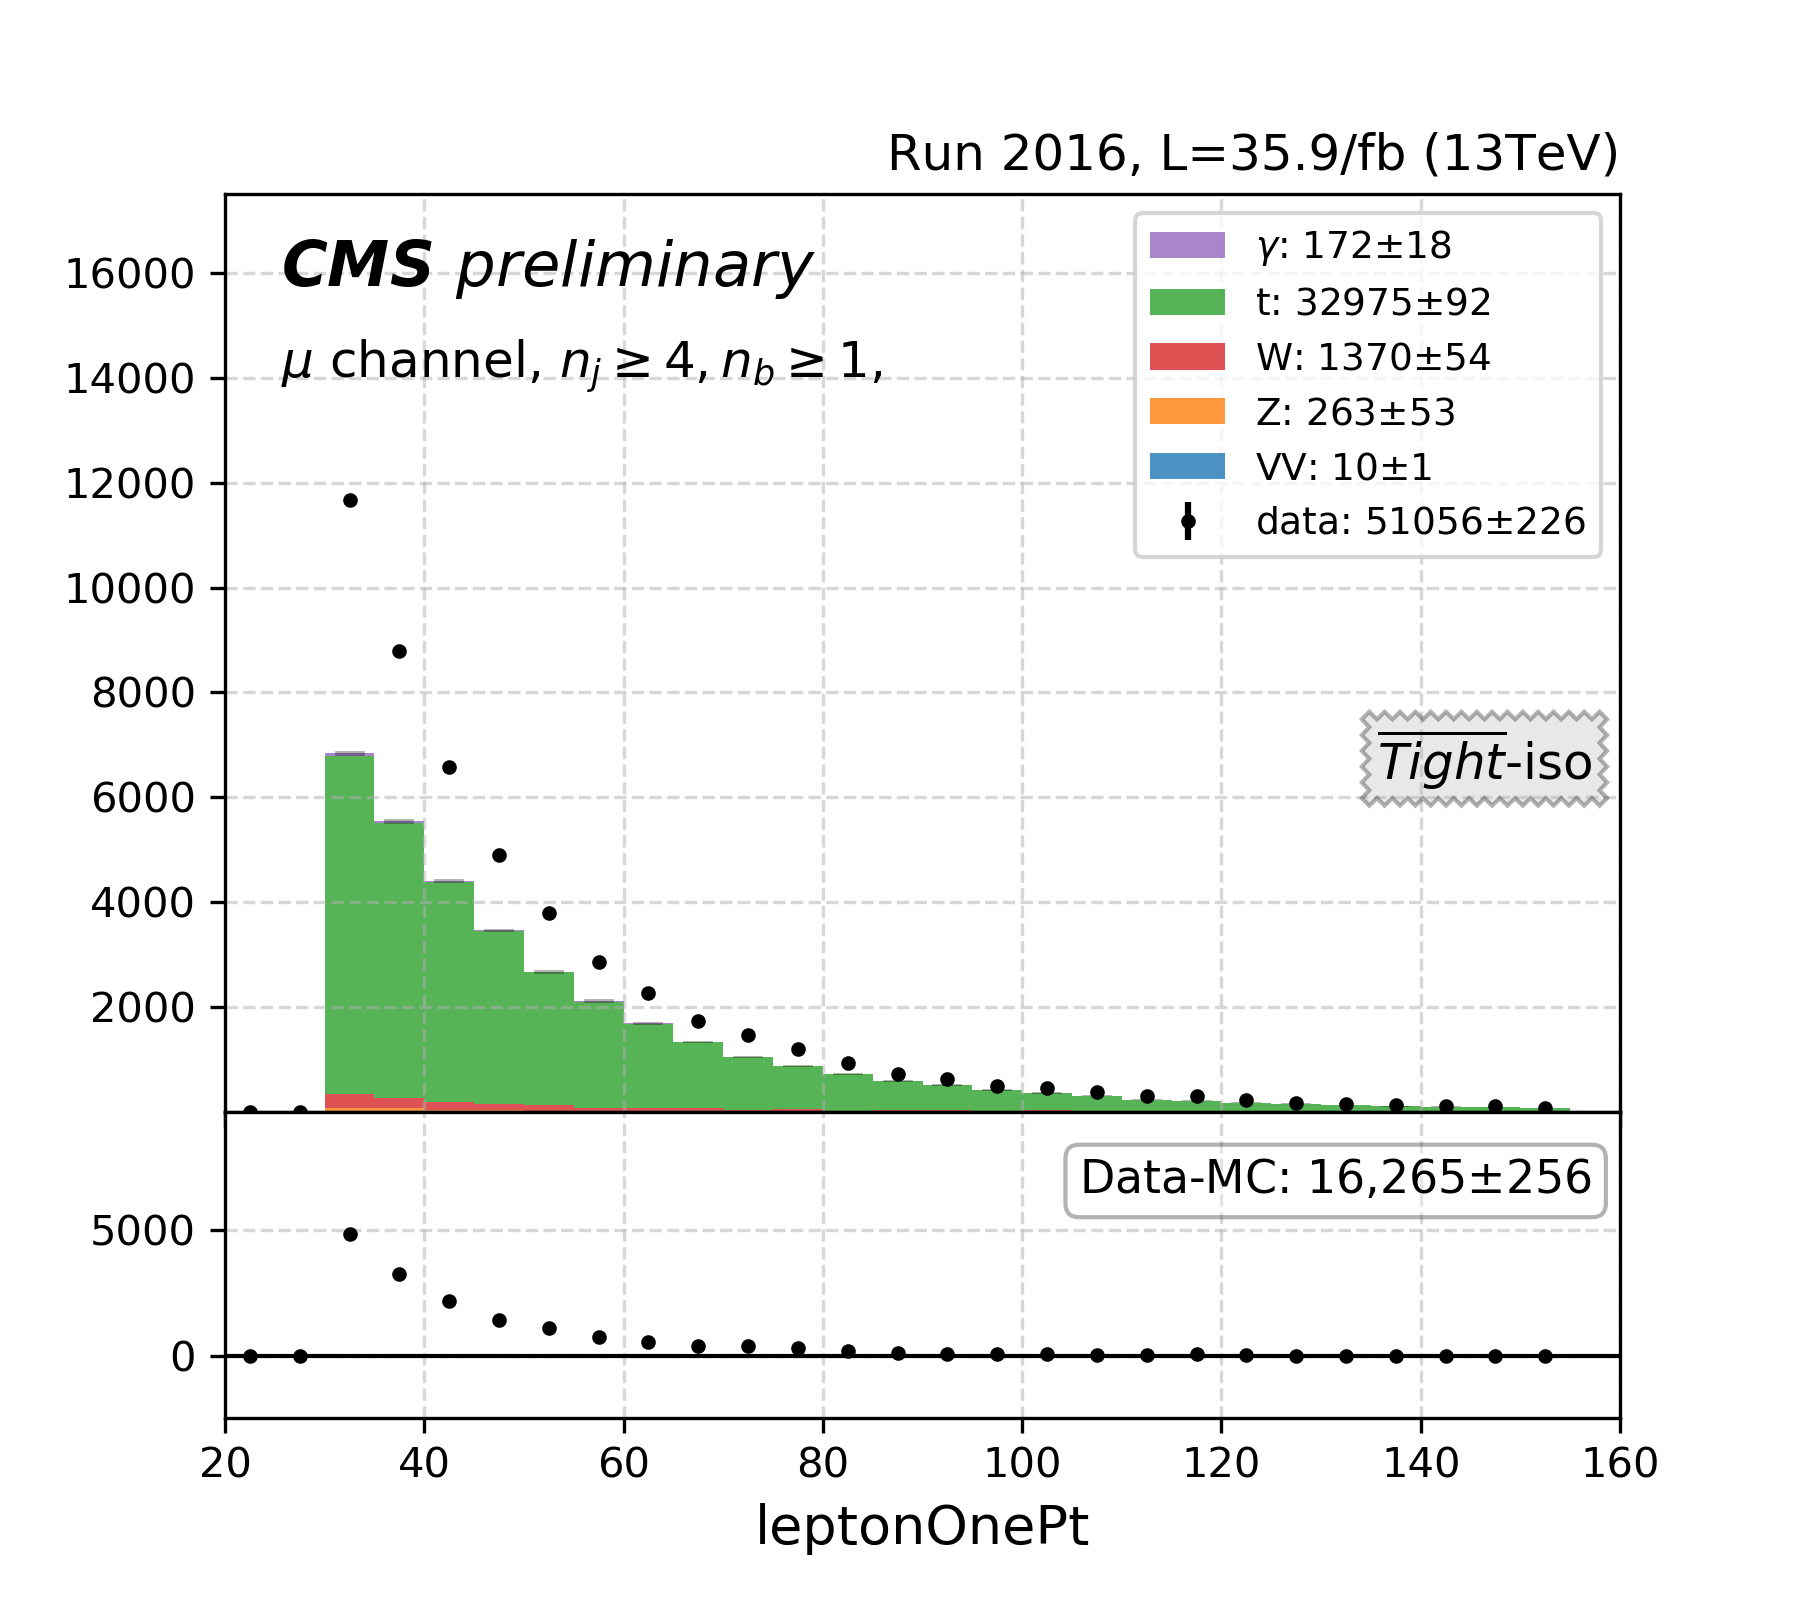
\includegraphics[width=0.24\textwidth]{appendices/qcdSF/figures/4j1b/mu_leptonOnePt_False.png}
    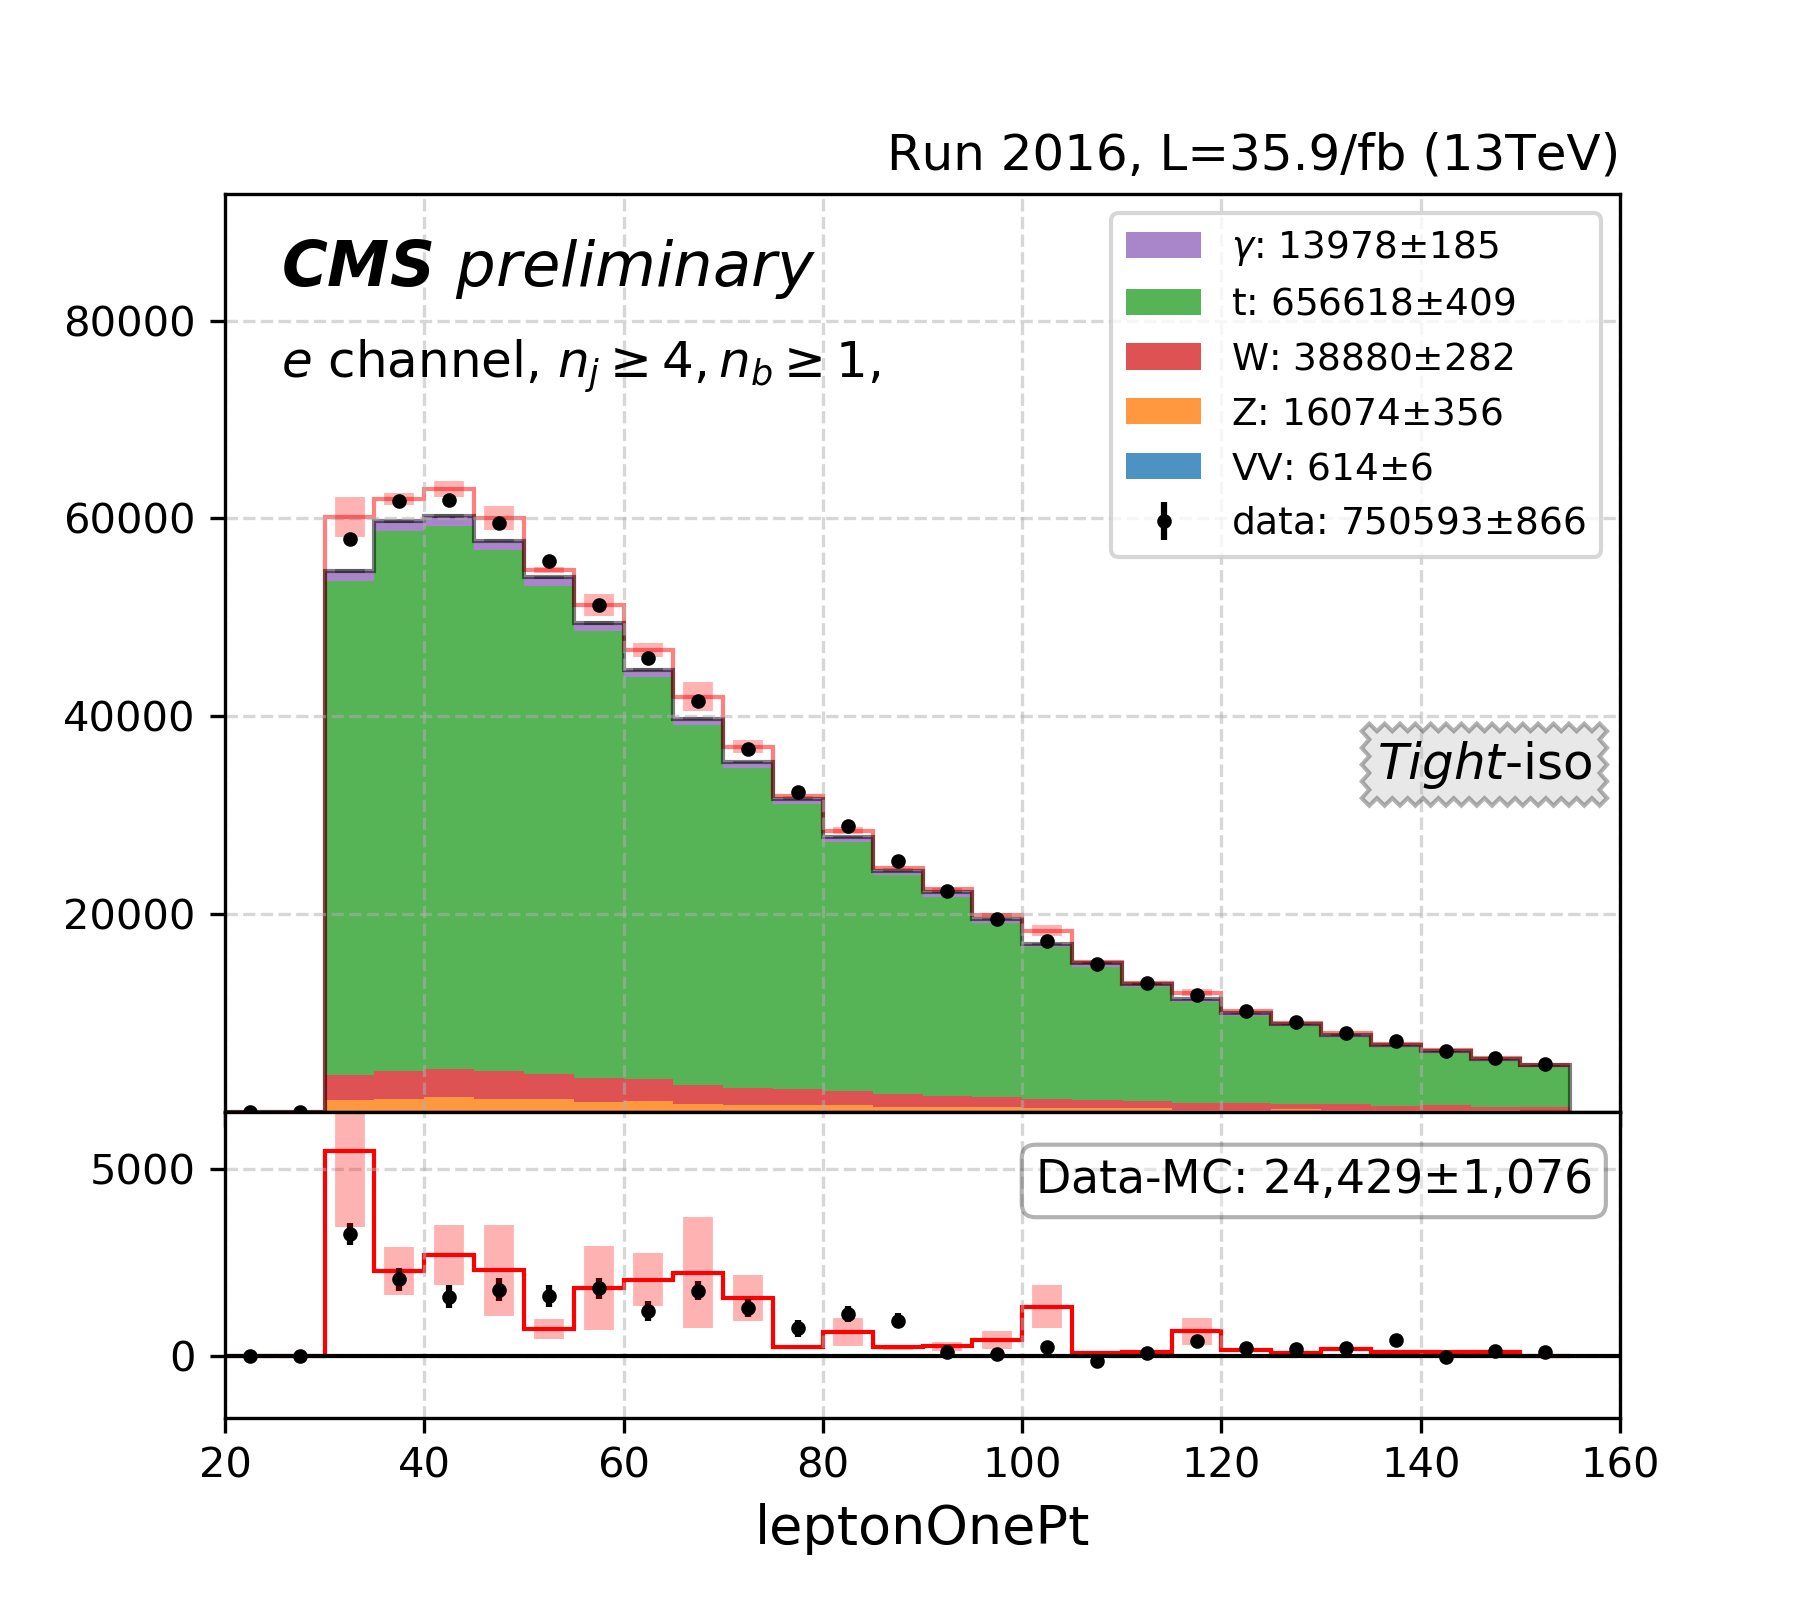
\includegraphics[width=0.24\textwidth]{appendices/qcdSF/figures/4j1b/e_leptonOnePt_True_mcqcd.png}
    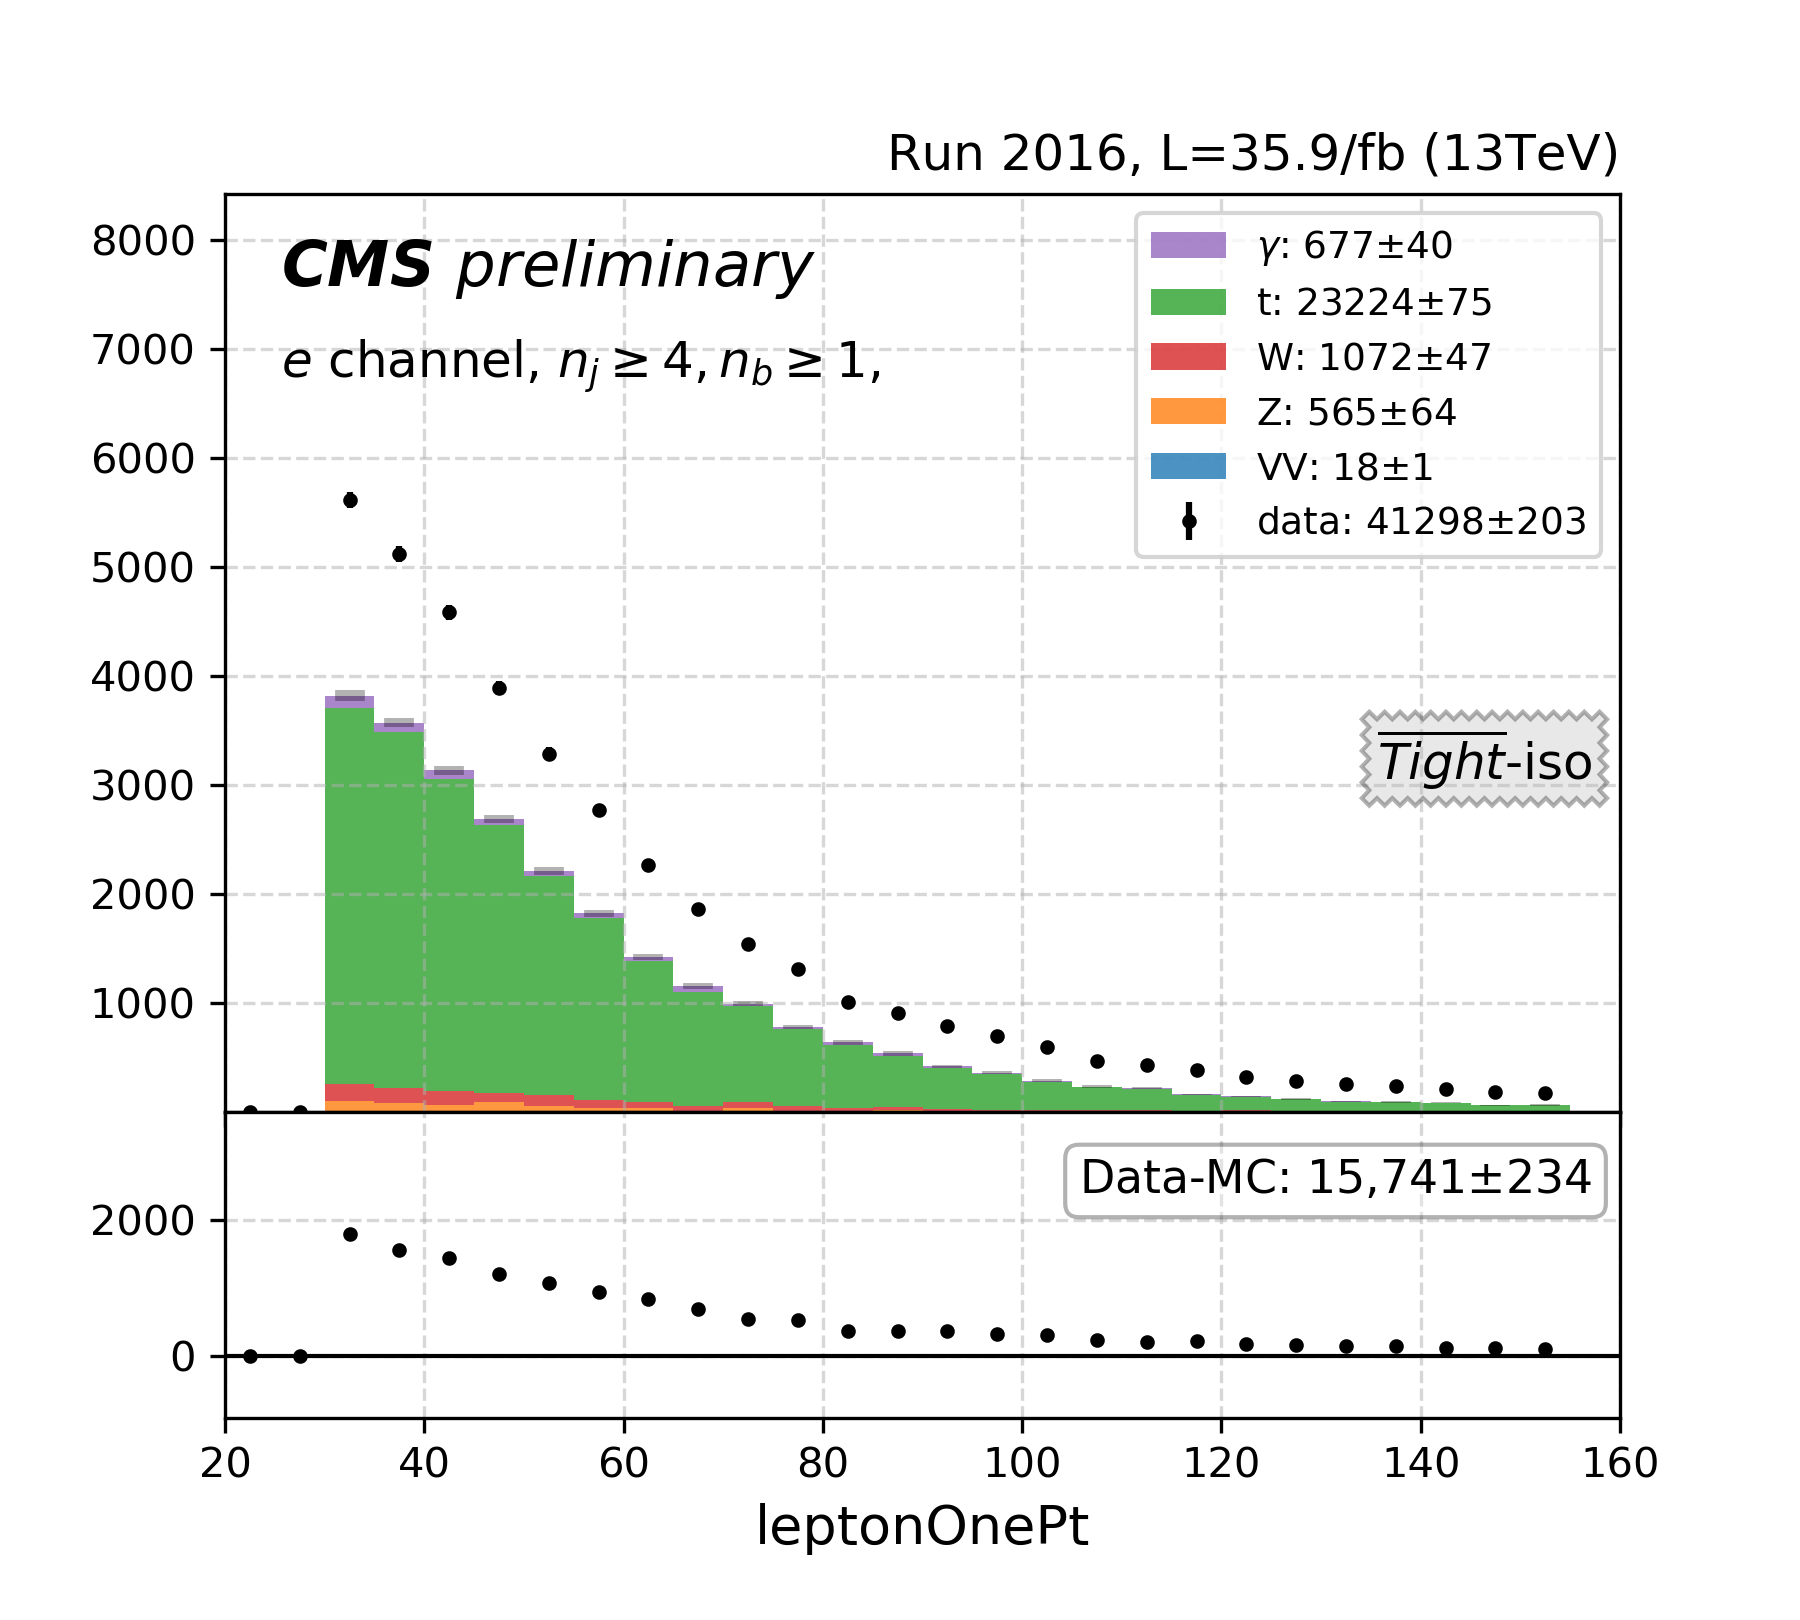
\includegraphics[width=0.24\textwidth]{appendices/qcdSF/figures/4j1b/e_leptonOnePt_False.png}
    
    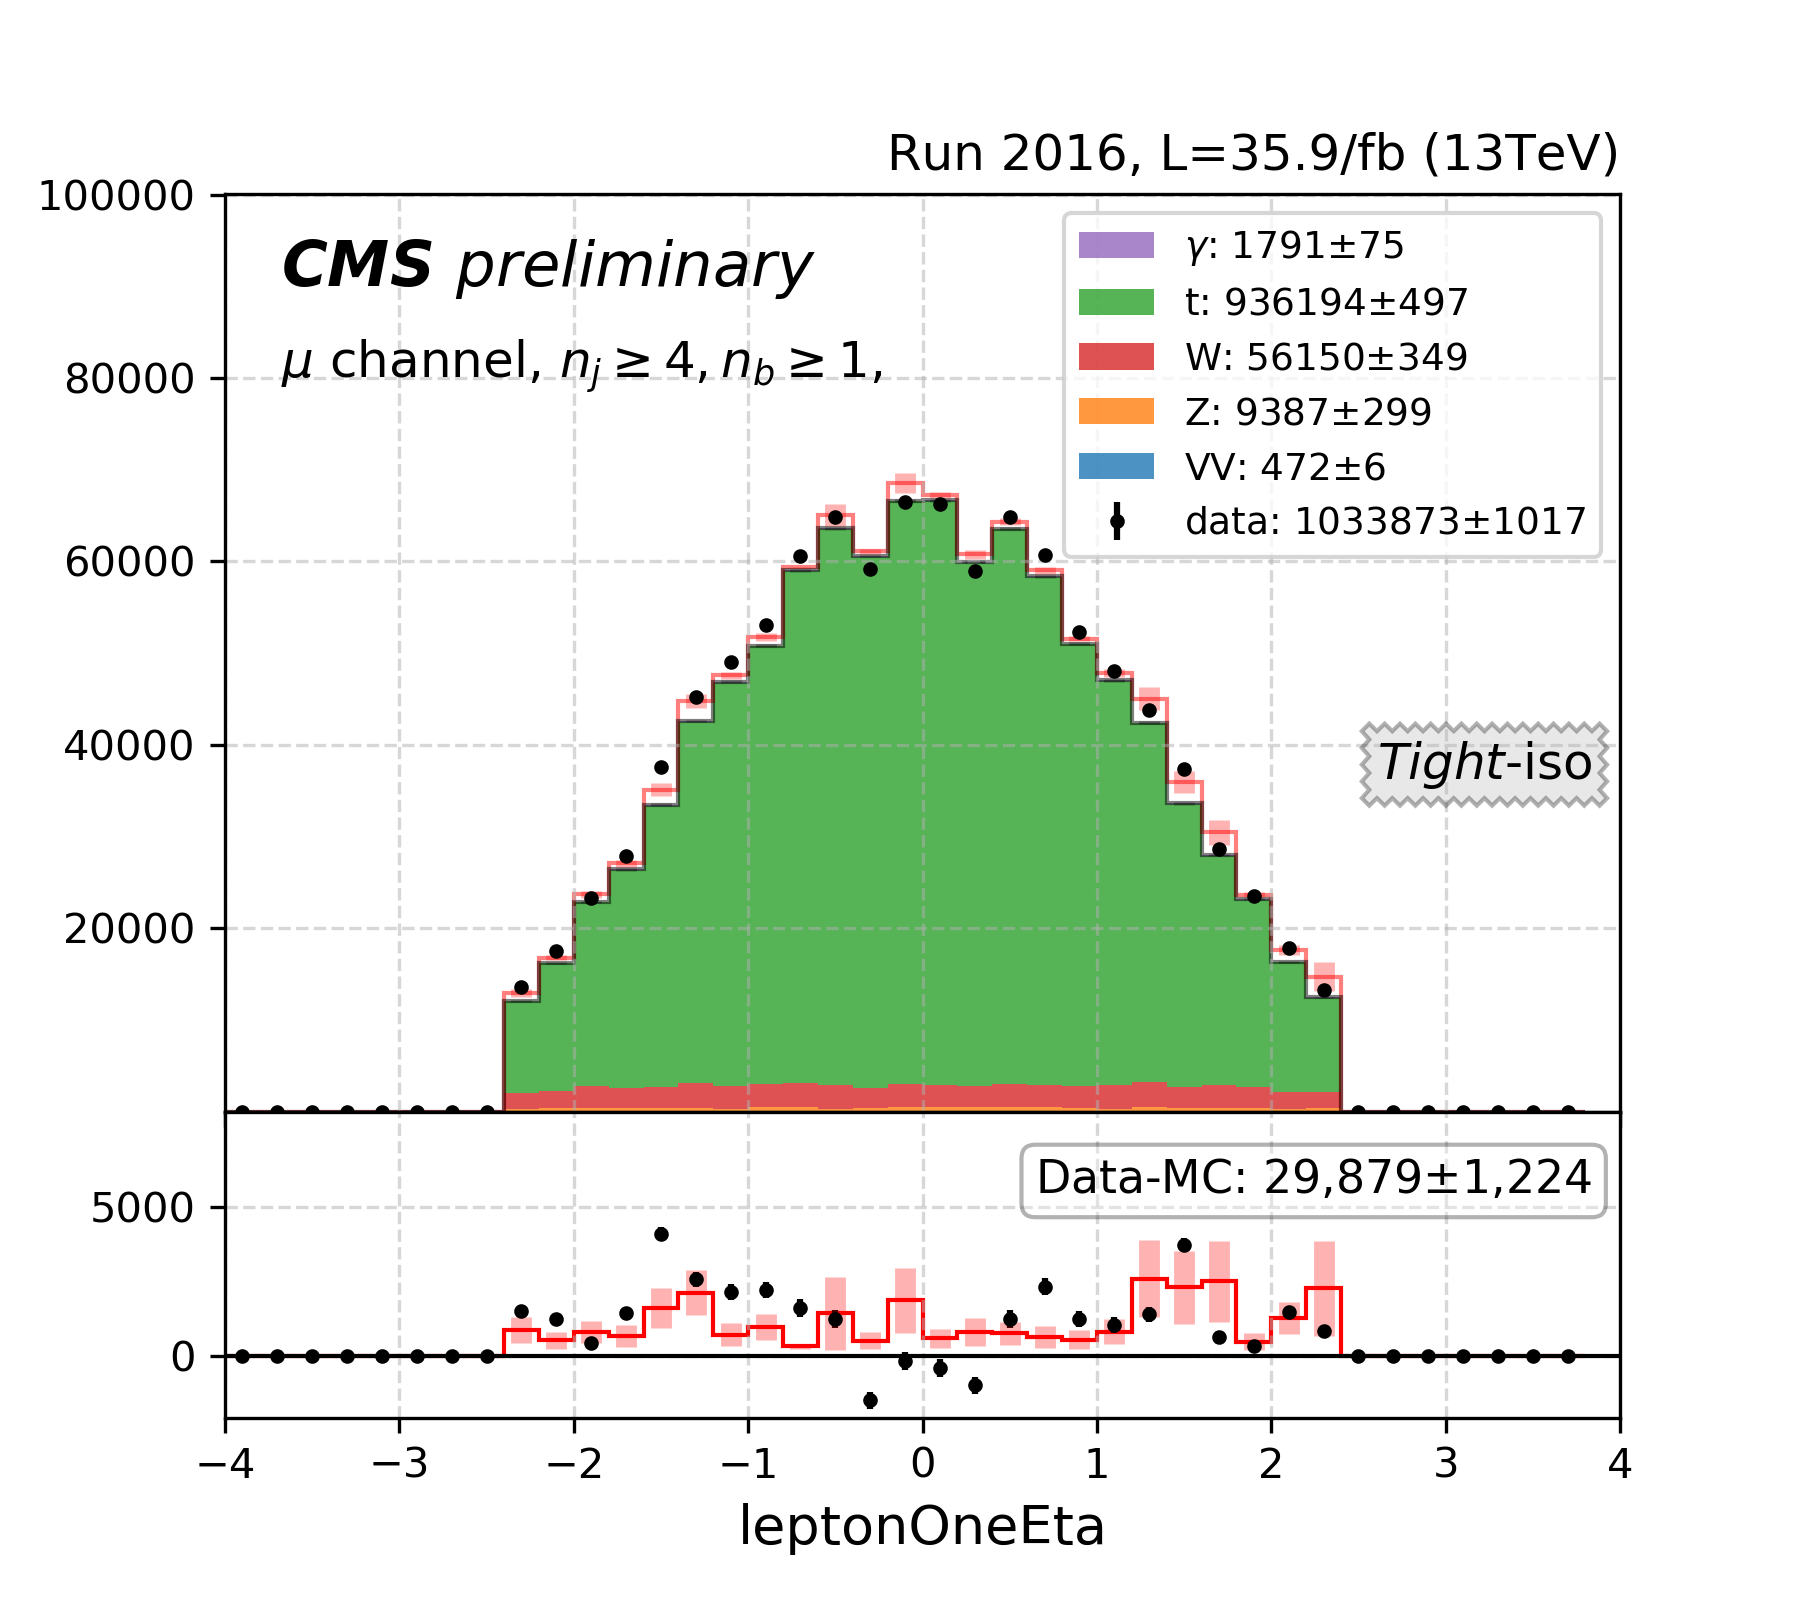
\includegraphics[width=0.24\textwidth]{appendices/qcdSF/figures/4j1b/mu_leptonOneEta_True_mcqcd.png}
    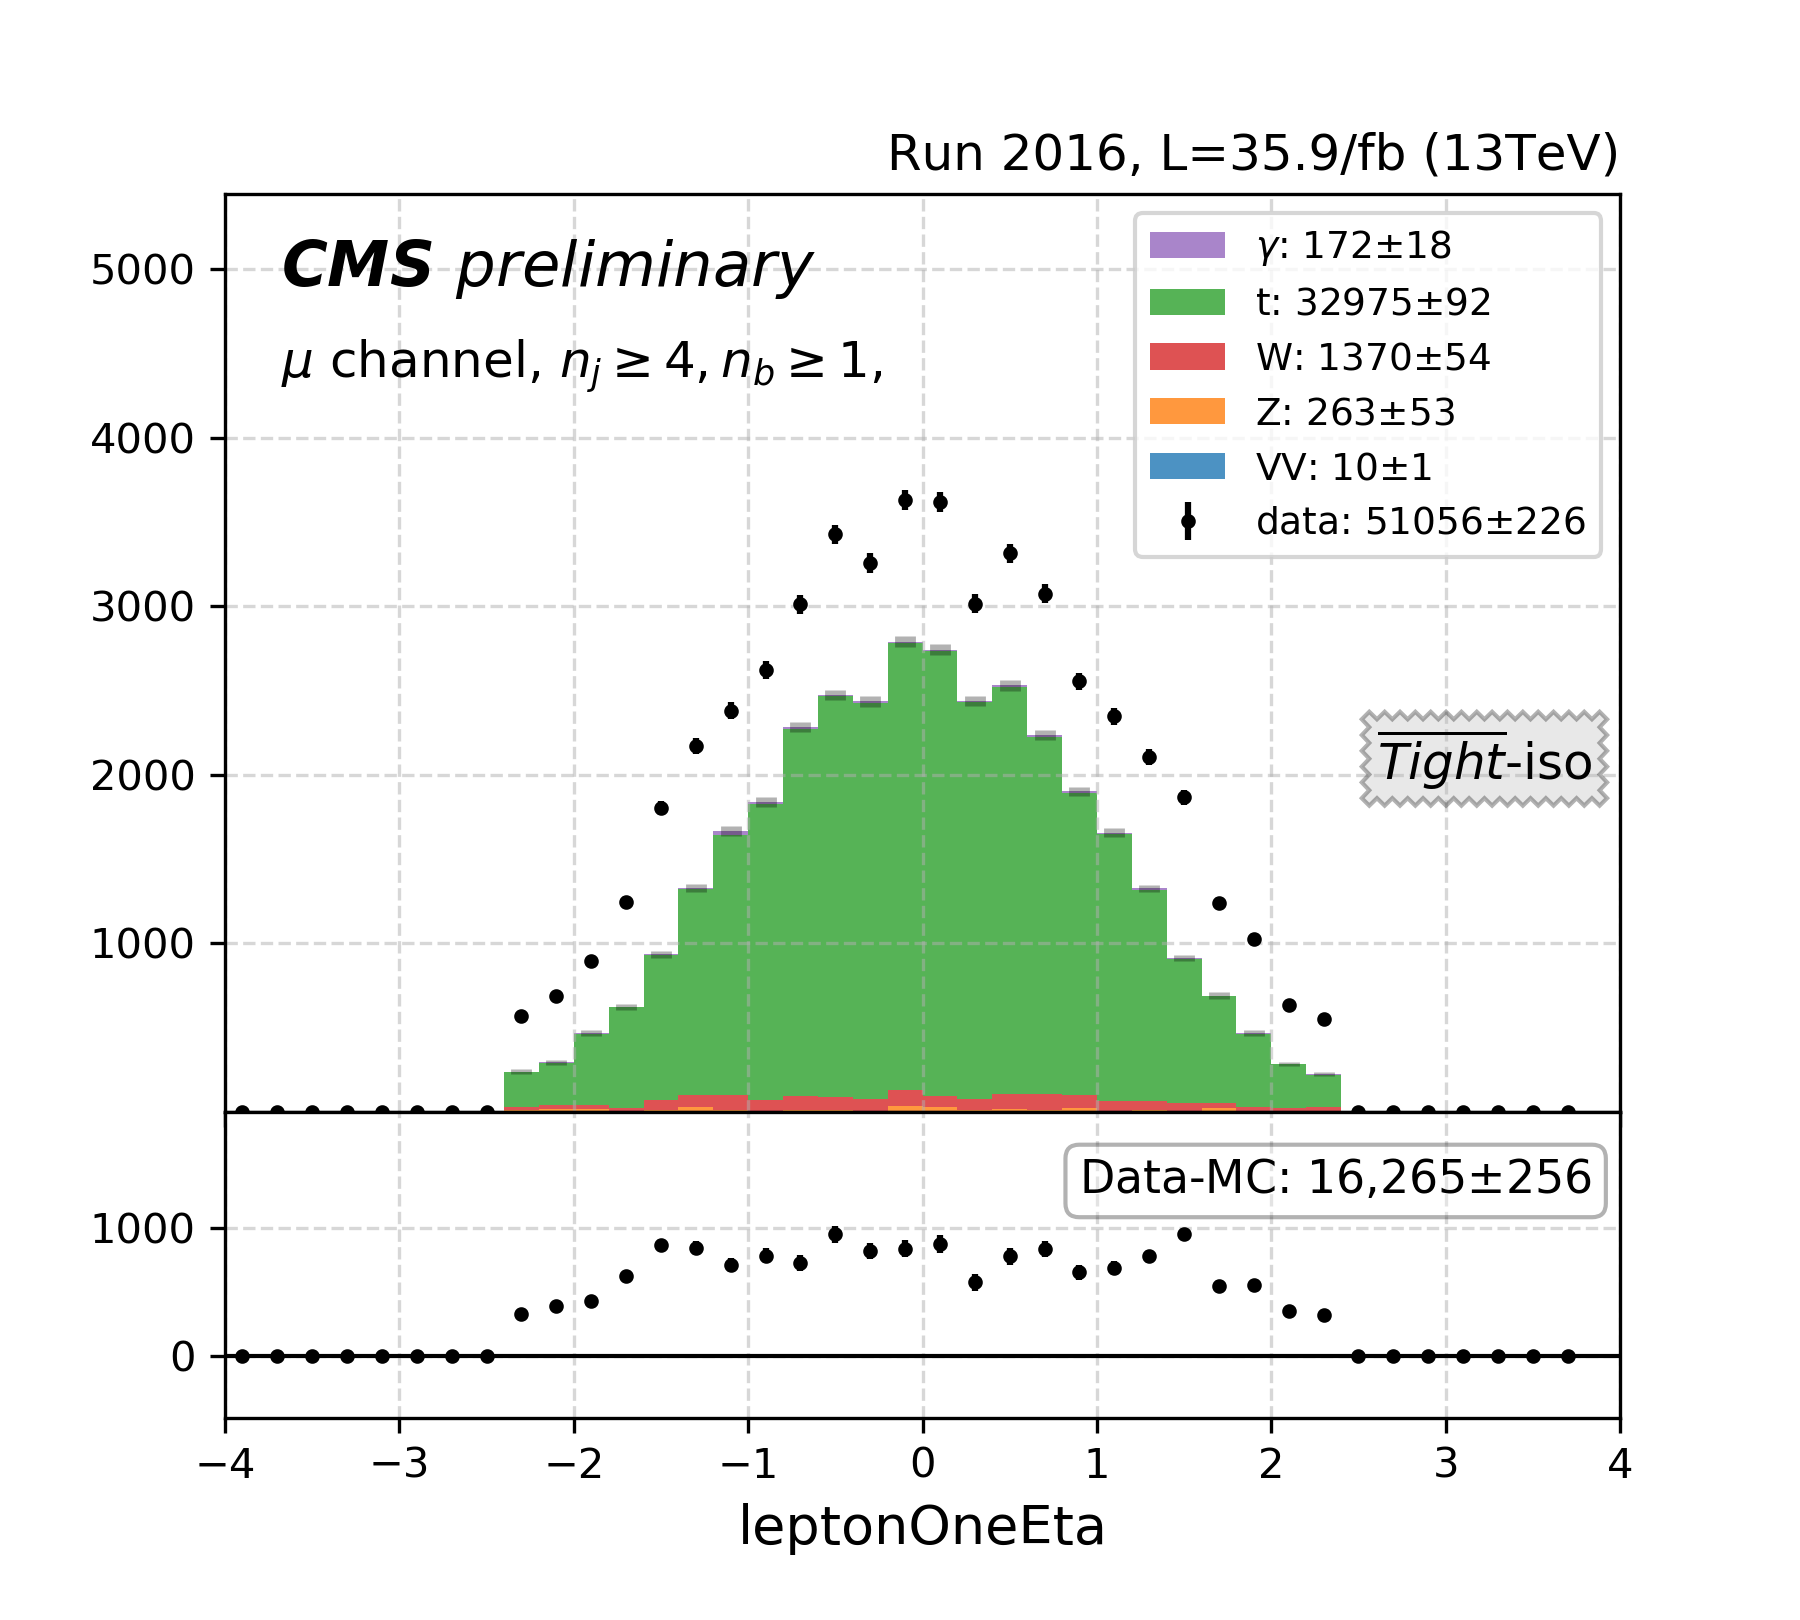
\includegraphics[width=0.24\textwidth]{appendices/qcdSF/figures/4j1b/mu_leptonOneEta_False.png}
    \includegraphics[width=0.24\textwidth]{appendices/qcdSF/figures/4j1b/e_leptonOneEta_True_mcqcd.png}
    \includegraphics[width=0.24\textwidth]{appendices/qcdSF/figures/4j1b/e_leptonOneEta_False.png}
    
    \includegraphics[width=0.24\textwidth]{appendices/qcdSF/figures/4j1b/mu_nJets_True_mcqcd.png}
    \includegraphics[width=0.24\textwidth]{appendices/qcdSF/figures/4j1b/mu_nJets_False.png}
    \includegraphics[width=0.24\textwidth]{appendices/qcdSF/figures/4j1b/e_nJets_True_mcqcd.png}
    \includegraphics[width=0.24\textwidth]{appendices/qcdSF/figures/4j1b/e_nJets_False.png}
    
    \includegraphics[width=0.24\textwidth]{appendices/qcdSF/figures/4j1b/mu_nBJets_True_mcqcd.png}
    \includegraphics[width=0.24\textwidth]{appendices/qcdSF/figures/4j1b/mu_nBJets_False.png}
    \includegraphics[width=0.24\textwidth]{appendices/qcdSF/figures/4j1b/e_nBJets_True_mcqcd.png}
    \includegraphics[width=0.24\textwidth]{appendices/qcdSF/figures/4j1b/e_nBJets_False.png}
    

    \caption{Reweight $\tau_h$ and $j \to \tau_h$ efficiencies in the dedicated FSR, ISF, MEPS, UE ttbar samples}
    \label{fig:appendix:4j1b}
\end{figure}